\documentclass[letterpaper,journal]{IEEEtran}
\usepackage{amsmath,amssymb,booktabs,array,url,cite}
\usepackage{microtype}
\usepackage{placeins}
\usepackage{xurl}
\usepackage{pgfplots}
\usepgfplotslibrary{groupplots}
\pgfplotsset{compat=1.18}
\usepackage[hidelinks]{hyperref}
\newcommand{\E}{\mathbb{E}}
\newcommand{\R}{\mathbb{R}}
\newcounter{allocationprocedure}
\newcounter{allocationstep}
\newenvironment{allocationprocedure}[2]{%
  \par\medskip\noindent\begin{minipage}{\linewidth}\small
  \refstepcounter{allocationprocedure}\label{proc:#1}%
  \hrule\smallskip\textbf{Allocation procedure \theallocationprocedure: #2}\par\smallskip
}{\par\smallskip\hrule\end{minipage}\par\medskip}
\newenvironment{allocationsteps}{%
  \begin{list}{\arabic{allocationstep}.}{\usecounter{allocationstep}%
  \setlength{\leftmargin}{1.5em}\setlength{\labelsep}{0.4em}%
  \setlength{\itemsep}{2pt}\setlength{\parsep}{0pt}\setlength{\topsep}{3pt}}%
}{\end{list}}
\begin{document}
\title{Low-Risk and Coskewness-Based Stock Selection:\\The Contributions of Signal Selection and Portfolio Weighting}
\author{Team \#4
\thanks{Hanyang University. Revised November 7, 2026.}}

\markboth{Introduction to Financial Engineering (INE3083), Portfolio Project Report}%
{Team 4: Low-Risk and Coskewness-Based Stock Selection}

\maketitle
% Keep short columns from stretching the spaces around intact procedures and floats.
\raggedbottom
\begin{abstract}
Does negative coskewness add to low-risk stock selection, and does optimization improve the resulting portfolio? We compare signal combinations under common constraints, then apply 19 weighting rules to the same 30 U.S.-listed stocks each month from February 2003 through December 2020. Adding negative coskewness to low beta and low volatility raises the full-period Sharpe ratio by 0.281 (95\% confidence interval 0.051 to 0.562), but also raises downside beta from 0.66 to 0.79. Capped value weighting earns 14.05\% annually after trading costs, versus 10.86\% for the CRSP value-weighted total-return market. Its Sharpe advantage over CRSP is significant over the full sample but not in 2012--2020. No alternative weighting rule delivers a higher compound return or a significant improvement in mean return after adjustment for multiple comparisons. In this sample, coskewness adds return at the cost of greater downside exposure; changing weights adds little under the baseline position limit.
\end{abstract}
\begin{IEEEkeywords}
Portfolio selection, low-risk investing, coskewness, covariance estimation, transaction costs, backtesting.
\end{IEEEkeywords}

\section{Overview}\label{sec:overview}
\subsection{Motivation}
\IEEEPARstart{A}{n} investor seeking lower equity risk can select less volatile stocks, give such stocks larger weights, or do both. These choices answer different questions. A selection signal can add return while increasing losses in bad months; a weighting rule can lower variance without improving terminal wealth. We study these trade-offs in a monthly U.S. equity strategy that ranks stocks on low beta, low volatility, and negative coskewness.

We first compare portfolios formed with and without each signal, holding stock count, retention, industry limits, position caps, and the trading-cost rate fixed. We then apply 19 weighting rules to the same monthly selection. Capped value weighting (Capped VW) is the allocation reference; the dividend-inclusive CRSP value-weighted market is the primary external benchmark. Only the first comparison changes which stocks qualify.

\subsection{Related Literature and Research Questions}
Leverage constraints offer one explanation for demand for high-beta stocks \cite{bab}. Systematic skewness provides a different rationale: investors may require compensation for holding stocks with adverse exposure to large market movements \cite{coskew}. Neither argument implies that selecting stocks with negative coskewness protects against a crash. We therefore examine both the return increment over a low-risk portfolio and the losses incurred in down markets.

Mean--variance theory gives weights for specified moments \cite{markowitz}; an investor must estimate those moments. Estimation error can offset the theoretical gains from optimization \cite{dgu}. Linear and nonlinear shrinkage address different sources of covariance error \cite{lw,qis}. We compare estimators under the same constraints, then vary the estimation window and position limit separately. Since the strategy followed an earlier search over signals and portfolio sizes \cite{overfit}, these comparisons describe realized performance; the later subsample is not an untouched test of signal discovery.

\subsection{Overall Investment Framework}
At the end of month $t$, observable characteristics determine eligibility and selection. The allocation rule sets weights for month $t+1$ using data through $t$ (Fig.~\ref{fig:framework}). Market regimes classify realized returns and never enter the investment rule.

\begin{figure*}[t]\centering
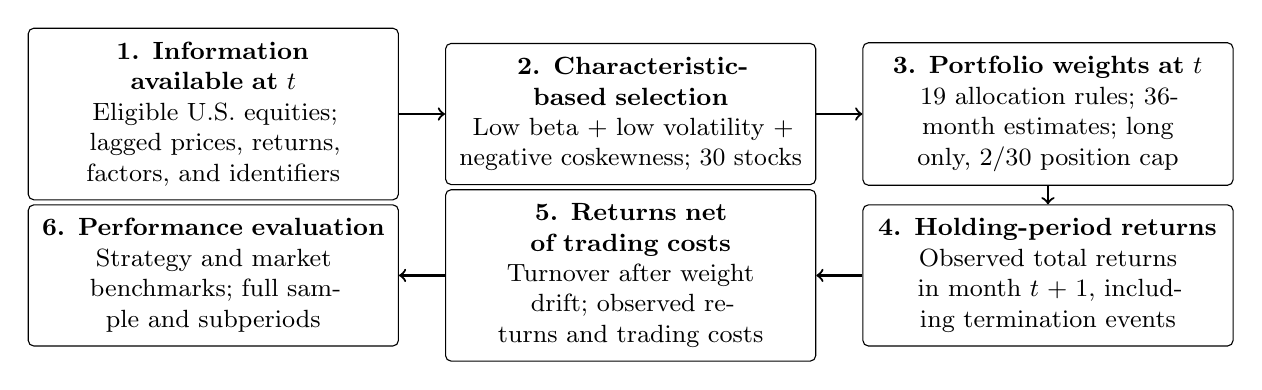
\begin{tikzpicture}[every node/.style={font=\small,align=center},box/.style={draw,rounded corners=2pt,text width=4.35cm,minimum height=1.35cm,inner sep=5pt}]
\node[box] (data) at (0,0) {\textbf{1. Information available at $t$}\\Eligible U.S. equities; lagged prices, returns, factors, and identifiers};
\node[box] (select) at (5.3,0) {\textbf{2. Characteristic-based selection}\\Low beta + low volatility + negative coskewness; 30 stocks};
\node[box] (allocate) at (10.6,0) {\textbf{3. Portfolio weights at $t$}\\19 allocation rules; 36-month estimates; long only, $2/30$ position cap};
\node[box] (hold) at (10.6,-2.05) {\textbf{4. Holding-period returns}\\Observed total returns in month $t+1$, including termination events};
\node[box] (account) at (5.3,-2.05) {\textbf{5. Returns net of trading costs}\\Turnover after weight drift; observed returns and trading costs};
\node[box] (evaluate) at (0,-2.05) {\textbf{6. Performance evaluation}\\Strategy and market benchmarks; full sample and subperiods};
\draw[->,thick] (data)--(select);\draw[->,thick] (select)--(allocate);
\draw[->,thick] (allocate)--(hold);\draw[->,thick] (hold)--(account);\draw[->,thick] (account)--(evaluate);
\end{tikzpicture}
\caption{Monthly portfolio construction. Signal comparisons vary Step 2 under common rules. Allocation comparisons hold Step 2 fixed and vary Step 3.}\label{fig:framework}
\end{figure*}

\section{Investment Universe}\label{sec:universe}
\subsection{Asset Pool and Eligibility}
The universe comprises common stocks on the NYSE, AMEX, and NASDAQ, regardless of issuer domicile. Stocks must have a price and trading volume in the rebalancing month. We exclude SPAC-like firms, delistings that month, and stocks below the contemporaneous 20th percentile of NYSE market capitalization across all three exchanges.

\subsection{Data Sources and Sample}
We match securities by PERMNO and month across the project price panel, the original CRSP monthly stock file, and the selection records. The evaluation covers 215 holding months from February 2003 through December 2020. At 30 stocks per month, the original selection contains 6,450 stock-months, each with its prior month-end scores, rank, and portfolio weight. Rerunning the selection rule reproduced all 6,450 records \cite{selectioncode}. The allocation comparison uses the original constituents and capitalization weights, preserving the recorded weights where the filtered metadata lack capitalization. For the sector analysis, we fill missing industry codes from the original CRSP \texttt{SICCD} field before grouping holdings by two-digit SIC.

The monthly Fama--French (FF) files supply factor returns and the risk-free rate. Expanded factor regressions and factor-covariance estimates also use AQR's U.S. monthly Betting Against Beta (BAB) series, downloaded November 3, 2026 \cite{bab,aqrbabdata}. BAB is an external long--short factor; the strategy returns are for long-only portfolios after trading costs.

\subsection{Return Pre-processing and Terminal Events}
For the allocation experiment, monthly stock returns come from the CRSP CIZ \texttt{MthRet} total-return field \cite{crsp}. We check the uniqueness of security-month keys and agreement between the original and cleaned returns wherever both are present. The original file supplies 1,109 stock-months absent from the cleaned extract: 1,086 ordinary observations for non-U.S.-incorporated issuers and 23 terminal observations. The terminal returns range from $-2.4164\%$ to $+9.1320\%$ and comprise 20 mergers and three exchange or reclassification events. After the observed terminal return, proceeds remain in cash until rebalancing. We do not add a second delisting return or impute a loss. Observed returns cover all 6,450 baseline holdings and all 28,470 distinct security-months needed for their 36-month estimation windows.

\subsection{Estimation, Validation, and Evaluation Timing}
At each month-end $t$, risk-based baseline rules use 36 monthly returns through $t$; all allocations earn returns in $t+1$. Thus the February 2000--January 2003 window determines weights for February 2003. Bayes--Stein also estimates expected returns. This rolling design produces out-of-sample returns relative to the allocation estimates. No separate validation set was used to select allocation parameters. The original strategy search considered several signals and portfolio sizes; reconstructing the monthly constituents does not undo that search. February 2003--December 2011 and January 2012--December 2020 are retrospective comparison periods. Neither provides an untouched test of the signal design.

\section{Portfolio Framework}\label{sec:framework}
\subsection{Economic Design of the Selection Rule}
\subsubsection{Risk and Return Characteristics}
Low beta ($B$) limits sensitivity to the market; low volatility ($V$) addresses total risk. Under $r_i=\alpha_i+\beta_i m+\varepsilon_i$, with $\operatorname{Cov}(m,\varepsilon_i)=0$, total variance is $\beta_i^2\operatorname{Var}(m)+\operatorname{Var}(\varepsilon_i)$. A low-beta stock can therefore retain substantial firm-specific risk. Leverage constraints and benchmark-related limits to arbitrage motivate studying these characteristics \cite{bab,baker}. A portfolio may benefit from lower volatility even when neither characteristic predicts higher raw returns.

Negative coskewness ($C$) has a different economic rationale. Investors who value positive portfolio skewness may demand compensation for holding stocks that lower it \cite{coskew}. This argument predicts neither a hedge against market declines nor a premium in every period. The empirical question is whether adding $C$ improves the risk--return trade-off of a portfolio already selected on $B$ and $V$.

\subsubsection{Signal Measurement}
The beta score uses monthly beta estimates based on daily returns. The rule bounds each estimate between $-3$ and $5$ and averages the preceding 12 months, requiring at least nine estimates. It ranks stocks on $0.6\overline\beta+0.4$, giving lower values higher scores. This positive affine transformation preserves ranks; only the estimation, bounding, and averaging steps can change their order. The volatility score ranks the sample standard deviation of the preceding 12 monthly returns in reverse order, requiring all 12 observations.

The coskewness score ranks
\begin{equation}
 C_{i,t}=-\frac{\E[(x_i-\overline x_i)(m-\overline m)^2]}
 {\sigma_{x_i}\sigma_m^2},
\end{equation}
where the moments use stock and market excess returns over the preceding 60 months, with at least 36 observations. A higher score denotes more negative coskewness. Squaring the market deviation gives weight to large moves in either direction. For centered excess returns $x_i=\beta_i m+\varepsilon_i$,
\begin{equation}
 \E[x_i m^2]=\beta_i\E[m^3]+\E[\varepsilon_i m^2].
\end{equation}
The signal thus contains a component related to market beta whenever the market is skewed. The analysis below concerns the raw standardized comoment. A residual-based score is a different specification; its performance has not been independently verified.

\subsubsection{Ranking and Portfolio Construction}
At each month-end, the rule averages the cross-sectional percentile ranks of the included signals. Ranks put all three characteristics on the same scale; equal weights avoid fitting coefficients to returns when two of the signals are intended to limit risk. Equal score weights imply neither equal risk contributions nor an optimal combination. The original strategy search also considered liquidity, issuance, and momentum \cite{teamrecord}.

The baseline selects $K=30$ stocks. An incumbent can remain if it ranks among the top 45 eligible stocks; open positions go to the highest-ranked eligible names, subject to at most nine holdings in each two-digit SIC industry. This is a limit on industry counts, not on industry weights. We cap each portfolio weight at $2/K$. To compare signals, we reselect stocks for each signal combination under the same rules, weight them by capped market capitalization, and deduct 20 basis points per round trip. To compare allocations, we instead hold the three-signal constituents fixed each month and change only their weights.

\subsubsection{Marginal Contribution of the Selection Signals}\label{sec:signalcomparisons}
Table~\ref{tab:archive}, Panel A, shows all seven nonempty combinations of $B$, $V$, and $C$. The three-signal portfolio has the highest full-period Sharpe ratio (1.11). The $B+V$ portfolio has lower volatility and market beta, while $C$ alone has the highest volatility and deepest drawdown. Investors who added $C$ to the two low-risk signals accepted more market exposure in exchange for higher realized returns.

\begin{table*}[t]\centering
\caption{Selection under matched portfolio rules. Panel A reports net Sharpe ratios, annualized volatility, maximum drawdown (MDD), and CAPM beta. Panel B compares the three-signal portfolio with $B+V$; mean differences are annualized percentage points, and the spanning regression controls for $B+V$ excess returns and the FF five factors. Parentheses contain HAC $t$ statistics. Sharpe intervals use 2,000 paired six-month block-bootstrap draws.}\label{tab:archive}
\small
\begin{tabular}{lrrrrrr}\toprule
\multicolumn{7}{l}{\textit{Panel A. Reconstructed characteristic portfolios}}\\
 & \multicolumn{3}{c}{Sharpe ratio} & & & \\
\cmidrule(lr){2-4}
Score & Full & 2003--11 & 2012--20 & Vol. (\%) & MDD (\%) & Beta\\\midrule
$B$       & 0.70 & 0.57 & 0.82 & 14.8 & $-35.2$ & 0.62\\
$V$       & 0.81 & 0.56 & 1.04 & 11.1 & $-36.8$ & 0.60\\
$C$       & 0.60 & 0.44 & 0.82 & 22.3 & $\underline{-64.0}$ & 1.30\\
$B+V$     & 0.83 & 0.72 & 0.93 & 10.3 & $-33.0$ & 0.47\\
$B+C$     & 0.92 & 1.02 & 0.81 & 13.9 & $-33.0$ & 0.76\\
$V+C$     & 0.86 & 0.77 & 0.93 & 13.4 & $-40.7$ & 0.80\\
$B+V+C$   & \textbf{1.11} & 1.09 & 1.12 & 11.4 & $-29.0$ & 0.62\\\midrule
\multicolumn{7}{l}{\textit{Panel B. Increment from adding negative coskewness to $B+V$}}\\
Period & \multicolumn{2}{c}{Mean difference ($t$)} & $\Delta$Sharpe & \multicolumn{2}{c}{95\% interval} & Ann. $\alpha$ (\%) ($t$)\\\midrule
Full & \multicolumn{2}{c}{4.12 (3.18)} & \textbf{0.281} & \multicolumn{2}{c}{$[0.051,0.562]$} & 4.04 (4.27)\\
2003--11 & \multicolumn{2}{c}{5.12 (3.12)} & 0.368 & \multicolumn{2}{c}{$[0.094,0.752]$} & 5.66 (4.12)\\
2012--20 & \multicolumn{2}{c}{3.12 (1.58)} & 0.194 & \multicolumn{2}{c}{$\underline{[-0.156,0.624]}$} & 2.12 (1.59)\\\bottomrule
\end{tabular}
\end{table*}

The net annualized mean-return gain from adding $C$ is 4.12 percentage points ($t=3.18$); the paired Sharpe gain is 0.281 (Panel B). The corresponding later-period interval includes zero, as does the interval for the change in the Sharpe gain between periods: $-0.174$ $[-0.697,0.380]$. The annualized mean gain falls by 2.00 percentage points ($t=-0.78$). We find a full-sample increment but cannot establish that the increment changed after 2011 or persists outside this sample. Selection comparisons use reconstructed returns; the baseline Sharpe is 1.111 on this series and 1.110 on the original allocation series. Market comparisons below retain the latter series.

Removing $B$, $V$, or $C$ reduces full-period Sharpe by 0.256, 0.189, or 0.281, respectively. Paired 95\% intervals for the removal effects exclude zero for $B$ and $C$, but every pairwise contrast between the three effects includes zero. The sample does not identify a single most important signal. Monthly Fama--MacBeth cross-sectional regressions of next-month returns on all three percentile scores \cite{famamacbeth} yield a mean monthly slope of about 0.5 percentage points per unit of the fractional rank of $C$ ($t\approx2.5$) and about $-0.05$ points for each low-risk score ($t\approx-0.1$). The $C$ slope falls to 0.20 points ($t=0.97$) in 2012--2020. A slope measures return predictability; unlike the portfolio Sharpe comparison, it does not reward a reduction in risk.

\subsubsection{Downside Risk and Specification Sensitivity}
Adding $C$ raises downside beta, estimated over negative market months, from 0.66 to 0.79. In the 22 months in the bottom market decile, the mean monthly portfolio return falls from $-3.29\%$ to $-4.02\%$; in the five worst market months it falls from $-7.10\%$ to $-9.30\%$. A shallower full-period MDD therefore does not imply better crash protection. In the seven worst market months of Crisis I, $B+V+C$ loses 36.56\% cumulatively versus 35.26\% for $B+V$; over the remaining 14 months it gains 24.87\% versus 16.60\%. The advantage comes from returns outside the worst months.

Across eight specifications varying $K$, incumbent retention, or the industry count limit, the full-period Sharpe increment from $C$ ranges from 0.068 to 0.288. The gain is 0.281 at $K=30$ but only 0.068 at $K=100$. For $K=40$, 50, and 100 the full-period MDD deepens rather than improves. The sign of the Sharpe increment is stable across these specifications; its size and drawdown consequences are not. These comparisons use the same historical sample and are not independent validations.

\subsubsection{Implications for the Allocation Stage}
Changing a selection score changes which stocks enter the portfolio. Changing an allocation rule can only redistribute capital among those already selected. The positive full-period increment from selecting on $C$ therefore does not imply that raising its portfolio-weighted score will improve returns within the selected 30. We test that distinction by comparing unconstrained score exposures with allocations that match the capped capitalization portfolio's three scores.

\subsection{Mathematical Specification and Common Constraints}\label{sec:allocation}
At each baseline rebalance $t$, $X_t\in\R^{T\times N}$ contains $T=36$ prior monthly returns in decimal units for the $N=30$ selected stocks. Define $\bar x=T^{-1}X_t'\mathbf1$, $Y=X_t-\mathbf1\bar x'$, $S=Y'Y/(T-1)$, and $S_0=Y'Y/T$. The divisor matters for shrinkage and mean estimation. A positive scalar multiple of the covariance matrix leaves GMVP weights unchanged.

The feasible set is the capped simplex
\begin{equation}\label{eq:feasible}
 \mathcal W_u=\{w\in\R^N:\mathbf1'w=1,\;0\leq w_i\leq u\},\qquad u=2/N.
\end{equation}
This set is compact and convex, and nonempty exactly when $Nu\geq1$. A positive semidefinite covariance matrix gives a convex variance objective; positive definiteness suffices for uniqueness. The 19 rules include two reference allocations and a norm-constrained GMVP that coincides with sample GMVP under the common cap.

\subsubsection{The Common Minimum-Variance Problem}
For a covariance estimate $\widehat\Sigma$, the GMVP solves the constrained Markowitz problem \cite{markowitz}
\begin{equation}\label{eq:gmvp}
 \min_{w\in\mathcal W_u} f(w),\qquad f(w)=w'\widehat\Sigma w.
\end{equation}
With nonsingular covariance and only the budget constraint, the solution is $\widehat\Sigma^{-1}\mathbf1/(\mathbf1'\widehat\Sigma^{-1}\mathbf1)$. Capping these weights after optimization does not generally solve \eqref{eq:gmvp}.

\subsection{Review of the Allocation Rules}\label{sec:allocationreview}
Eight GMVP specifications vary the covariance estimator. Two rules weight stocks by marginal risk; four others target risk budgets, diversification, estimated Sharpe, or tail loss. The remaining variants mix weights, constrain concentration, or penalize trades. Capped VW and equal weighting provide the allocation references in Table~\ref{tab:main}.

Sections~\ref{sec:covestimators}--\ref{sec:numerics} give the estimator formulas and numerical checks. The following procedures use the same ordered stock list $I_t$ and return matrix; results use observed CRSP returns and 20-basis-point round-trip costs.

Write $[z]_a^b=\min\{b,\max\{a,z\}\}$ for scalar truncation and $\Pi_{\mathcal W_u}$ for Euclidean projection onto the capped simplex.

$\operatorname{GMV}(\Sigma,u)$ calls \hyperref[alg:prox]{Algorithm 2} with zero trading penalty, equal initial weights, a 5,000-iteration limit, and a maximum absolute weight-change tolerance of $10^{-10}$. $\operatorname{Validate}$ requires $N$ finite weights, budget error at most $10^{-6}$, and weights in $[-10^{-7},u+10^{-6}]$. Only after acceptance does it set $w_i\leftarrow\max(w_i,0)$ and normalize $w\leftarrow w/(\mathbf1'w)$ in stock-list order. These checks concern feasibility; Appendix~\ref{app:replication} reports optimality tests.

\subsubsection{Market-Capitalization Weighting with a Position Limit}\label{alloc:source_weight}
Capped VW allocates in proportion to the selected firms' capitalizations until a stock reaches the position limit. Value weighting is a conventional reference for active allocation \cite{brandtppp} and requires no return-moment estimates.

For rebalance-date capitalizations $M_{i,t}>0$, the uncapped shares are $M_{i,t}/\sum_{j\in I_t}M_{j,t}$. Preserving relative capitalization among uncapped stocks gives
\begin{equation}\label{eq:marketcap}
 w_{i,t}=\min\{u,a_t M_{i,t}\},\qquad
 \sum_{i\in I_t} w_{i,t}=1,
\end{equation}
where $a_t>0$ redistributes the residual capital proportionally. MSCI uses a proportional redistribution convention \cite{mscicap}; we do not replicate its free-float index. The cap $u=2/30$ (6.67\%) is a design choice, not an optimum established by either source.

The backtest uses the recorded targets \cite{teamrecord}, projecting them onto $\mathcal W_u$ only to correct six-decimal rounding. Projecting the \emph{uncapped} shares instead would generally change their relative proportions. Section~\ref{sec:selectionrisk} checks the targets against rebalance-date capitalizations.

\begin{allocationprocedure}{source_weight}{Capped VW}
\textbf{Input:} Recorded weights $q_t$, constituent identifiers $I_t$, and cap $u$.
\begin{allocationsteps}
\item Align $q_t$ to the ordered identifiers in $I_t$. Require finite recorded weights and a total satisfying $|\mathbf1^{\prime}q_t-1|\leq2\times10^{-5}$.
\item Find $\tau$ such that $\sum_i[q_{i,t}-\tau]_0^u=1$.
\item Set $w_{i,t}\leftarrow[q_{i,t}-\tau]_0^u$. This reproduces the recorded allocation up to rounding; no capitalization estimate enters this step.
\item Return $\operatorname{Validate}(w_t)$.
\end{allocationsteps}
\textbf{Output:} Target weights $w_t$ for the next holding month.
\end{allocationprocedure}

\subsubsection{Equal Weighting}\label{alloc:equal_weight}
Equal weighting sets every target to $1/30$, preserving the equally weighted means of the selected scores and maximizing the effective number of holdings. It avoids estimating allocation parameters, a useful benchmark when estimation costs can erase diversification gains \cite{dgu}. Equal capital need not imply equal risk. Selection still depends on estimated signals, and constituent changes and price drift still induce trades.

\begin{allocationprocedure}{equal_weight}{Equal weighting}
\textbf{Input:} Constituent identifiers $I_t$ and cap $u$.
\begin{allocationsteps}
\item Set $N\leftarrow |I_t|$; require $Nu\geq1$.
\item For each $i=1,\ldots,N$, set $w_{i,t}\leftarrow1/N$.
\item Return $\operatorname{Validate}(w_t)$.
\end{allocationsteps}
\textbf{Output:} Target weights $w_t$ for the next holding month.
\end{allocationprocedure}

\subsubsection{Sample GMVP}\label{alloc:gmvp_sample}
Sample GMVP uses $S$ in \eqref{eq:gmvp} without forecasting means \cite{markowitz}. It may therefore hold a volatile stock with low covariance against the rest of the portfolio. With 465 distinct covariance entries estimated from 36 observations, small eigenvalues can magnify sampling error. The position cap limits extreme weights but cannot remove that error or the turnover it induces.

\begin{allocationprocedure}{gmvp_sample}{Sample GMVP}
\textbf{Input:} Historical return matrix $X_t$ and cap $u$.
\begin{allocationsteps}
\item Compute $\bar x\leftarrow X_t^{\prime}\mathbf1/T$ and $Y\leftarrow X_t-\mathbf1\bar x^{\prime}$.
\item Set $S\leftarrow Y^{\prime}Y/(T-1)$.
\item Set $w_t\leftarrow\operatorname{GMV}(S,u)$; return $\operatorname{Validate}(w_t)$.
\end{allocationsteps}
\textbf{Output:} Target weights $w_t$ for the next holding month.
\end{allocationprocedure}

\subsubsection{Constant-Correlation GMVP}\label{alloc:gmvp_constant_corr}
Constant correlation preserves each stock's variance but replaces all pairwise correlations by their common average \cite{constantcorr,lw}. This restriction economizes on correlation estimates at the cost of suppressing systematic differences across industries or stock pairs. The resulting GMVP generally differs from inverse volatility; its weights still reflect the common covariance term in \eqref{eq:cc}.

\begin{allocationprocedure}{gmvp_constant_corr}{Constant-correlation GMVP}
\textbf{Input:} Sample covariance $S$ and cap $u$.
\begin{allocationsteps}
\item Set $\sigma_i\leftarrow\sqrt{S_{ii}}$ and $C_{ij}\leftarrow S_{ij}/(\sigma_i\sigma_j)$.
\item Compute $\bar\rho\leftarrow\sum_{i\ne j}C_{ij}/[N(N-1)]$.
\item Set $F_{ii}\leftarrow S_{ii}$ and $F_{ij}\leftarrow\bar\rho\sigma_i\sigma_j$ for $i\ne j$.
\item Set $w_t\leftarrow\operatorname{GMV}(F,u)$; return $\operatorname{Validate}(w_t)$.
\end{allocationsteps}
\textbf{Output:} Target weights $w_t$ for the next holding month.
\end{allocationprocedure}

\subsubsection{Ledoit--Wolf Constant-Correlation GMVP}\label{alloc:gmvp_lw_constant_corr}
Ledoit--Wolf shrinkage combines sample covariance with the constant-correlation target \cite{lw}. Its estimated intensity accounts for sampling error shared by the two matrices. The endpoints recover sample and constant-correlation GMVP up to covariance scale. Both preserve marginal variances; only the estimated cross-stock dependence changes. The derivation requires temporal independence, finite fourth moments, and asymptotic regularity, assumptions that a short financial sample need not approximate well.

\begin{allocationprocedure}{gmvp_lw_constant_corr}{LW constant-correlation GMVP}
\textbf{Input:} Centered returns $Y$ and cap $u$; noncoincident sample and target matrices.
\begin{allocationsteps}
\item Set $S_0\leftarrow Y^{\prime}Y/T$, $v_i\leftarrow(S_0)_{ii}$, and $\sigma_i\leftarrow\sqrt{v_i}$. Construct $F_0$ by steps 1--3 of Procedure~\ref{proc:gmvp_constant_corr}, using $S_0$ in place of $S$.
\item For each pair $(i,j)$, compute $P_{ij}\leftarrow T^{-1}\sum_s y_{si}^2y_{sj}^2-(S_0)_{ij}^2$ and $\Theta_{ij}\leftarrow T^{-1}\sum_s y_{si}^3y_{sj}-v_i(S_0)_{ij}$. Set $\Theta_{ii}\leftarrow0$.
\item Set $\widehat\pi\leftarrow\sum_{ij}P_{ij}$ and $\widehat\rho\leftarrow\sum_iP_{ii}+\bar\rho\sum_{i\ne j}(\sigma_j/\sigma_i)\Theta_{ij}$.
\item Compute $\widehat\gamma\leftarrow\|F_0-S_0\|_F^2$ and $\delta\leftarrow[(\widehat\pi-\widehat\rho)/(T\widehat\gamma)]_0^1$.
\item Set $\widehat\Sigma\leftarrow\delta F_0+(1-\delta)S_0$ and $w_t\leftarrow\operatorname{GMV}(\widehat\Sigma,u)$. Return $\operatorname{Validate}(w_t)$.
\end{allocationsteps}
\textbf{Output:} Target weights $w_t$ for the next holding month.
\end{allocationprocedure}

\subsubsection{Ledoit--Wolf Identity GMVP}\label{alloc:gmvp_lw_identity}
Ledoit--Wolf identity shrinkage targets a scaled identity matrix under quadratic covariance loss \cite{identity}. Raising small eigenvalues limits reliance on apparently low-risk directions. Unlike constant-correlation shrinkage, it also compresses marginal volatility differences. Full shrinkage gives equal variances, zero covariances, and equal GMVP weights. The shrinkage intensity is estimated rather than fixed.

\begin{allocationprocedure}{gmvp_lw_identity}{LW identity GMVP}
\textbf{Input:} Centered returns $Y$ and cap $u$.
\begin{allocationsteps}
\item Set $S_0\leftarrow Y^{\prime}Y/T$, $m\leftarrow\operatorname{tr}(S_0)/N$, and $d^2\leftarrow\|S_0-mI\|_F^2$.
\item Compute $\bar b^2\leftarrow T^{-2}\sum_s\|y_sy_s^{\prime}-S_0\|_F^2$.
\item If $d^2=0$, set $\delta\leftarrow1$; otherwise set $\delta\leftarrow\min\{\bar b^2,d^2\}/d^2$.
\item Set $\widehat\Sigma\leftarrow(1-\delta)S_0+\delta mI$.
\item Set $w_t\leftarrow\operatorname{GMV}(\widehat\Sigma,u)$; return $\operatorname{Validate}(w_t)$.
\end{allocationsteps}
\textbf{Output:} Target weights $w_t$ for the next holding month.
\end{allocationprocedure}

\subsubsection{Ridge GMVP}\label{alloc:gmvp_ridge}
Ridge GMVP adds a scaled identity to $S$, or equivalently penalizes the squared norm of the weights \cite{norm,identity}. The fixed coefficient 0.3 in \eqref{eq:ridge} corresponds to identity shrinkage of $0.3/1.3$ for GMVP weights. It penalizes concentration, not changes from current holdings; its effect depends on the covariance spectrum. It differs from both estimated shrinkage and direct regularization of inverse covariance \cite{kourtis}.

\begin{allocationprocedure}{gmvp_ridge}{Ridge GMVP}
\textbf{Input:} Sample covariance $S$, cap $u$, and fixed coefficient $\kappa=0.3$.
\begin{allocationsteps}
\item Compute $m\leftarrow\operatorname{tr}(S)/N$.
\item Set $\widehat\Sigma\leftarrow S+\kappa mI$. Do not estimate $\kappa$ from realized holding-period returns.
\item Set $w_t\leftarrow\operatorname{GMV}(\widehat\Sigma,u)$; return $\operatorname{Validate}(w_t)$.
\end{allocationsteps}
\textbf{Output:} Target weights $w_t$ for the next holding month.
\end{allocationprocedure}

\subsubsection{RMT-Clipping GMVP}\label{alloc:gmvp_rmt_clipping}
Random-matrix filtering pools correlation eigenvalues below a noise boundary, renormalizes the correlation diagonal, and restores marginal variances \cite{rmt,rmtclean}. Unlike QIS's continuous eigenvalue corrections, the filter uses a threshold. Unit noise variance and the $N/T$ boundary are modeling assumptions: short samples, serial dependence, and time-varying volatility can put genuine dependence below the cutoff.

\begin{allocationprocedure}{gmvp_rmt_clipping}{RMT-clipping GMVP}
\textbf{Input:} Sample covariance $S$, sample length $T$, and cap $u$.
\begin{allocationsteps}
\item Set $\sigma_i\leftarrow\sqrt{S_{ii}}$ and $C_{ij}\leftarrow S_{ij}/(\sigma_i\sigma_j)$. Diagonalize $C=U\operatorname{diag}(\lambda)U^{\prime}$.
\item Set $\lambda_+\leftarrow(1+\sqrt{N/T})^2$ and $J\leftarrow\{j:\lambda_j<\lambda_+\}$.
\item Initialize $\widetilde\lambda\leftarrow\lambda$. If $J\ne\varnothing$, set $\widetilde\lambda_j\leftarrow |J|^{-1}\sum_{k\in J}\lambda_k$ for every $j\in J$.
\item Form $A\leftarrow U\operatorname{diag}(\widetilde\lambda)U^{\prime}$ and $h_i\leftarrow\sqrt{A_{ii}}$.
\item Set $\widehat\Sigma_{ij}\leftarrow A_{ij}\sigma_i\sigma_j/(h_i h_j)$. This restores marginal variances after correlation filtering.
\item Set $w_t\leftarrow\operatorname{GMV}(\widehat\Sigma,u)$; return $\operatorname{Validate}(w_t)$.
\end{allocationsteps}
\textbf{Output:} Target weights $w_t$ for the next holding month.
\end{allocationprocedure}

\subsubsection{Quadratic Inverse Shrinkage (QIS) GMVP}\label{alloc:gmvp_qis}
QIS retains sample covariance eigenvectors and applies nonlinear, direction-specific corrections to the eigenvalues \cite{qis}. It addresses eigenvalue dispersion but not eigenvector error; neither trading costs nor selection scores enter its loss criterion. Section~\ref{sec:covestimators} gives the spectral and moment conditions. Published author code supplies a numerical reference \cite{lwcode}.

\begin{allocationprocedure}{gmvp_qis}{QIS GMVP}
\textbf{Input:} Sample covariance $S$, sample length $T$, and cap $u$.
\begin{allocationsteps}
\item Set $n\leftarrow T-1$, $c\leftarrow N/n$, and $k\leftarrow\min(N,n)$. Diagonalize $S=U\operatorname{diag}(\lambda)U^{\prime}$ in ascending eigenvalue order; remove negative numerical roundoff by $\lambda_j\leftarrow\max(\lambda_j,0)$.
\item For $j=1,\ldots,k$, set $a_j\leftarrow1/\max(\lambda_{N-k+j},10^{-12})$. Set $h\leftarrow\min(c^2,c^{-2})^{0.35}N^{-0.35}$.
\item For every $(i,j)$, set $K_{ij}\leftarrow(a_i-a_j)^2+h^2a_i^2$. For each $j$, compute $\theta_j\leftarrow k^{-1}\sum_i a_i(a_i-a_j)/K_{ij}$ and $\psi_j\leftarrow k^{-1}\sum_i ha_i^2/K_{ij}$.
\item If $N\leq n$, set $d_j\leftarrow\{a_j[(1-c)^2+2c(1-c)\theta_j+c^2(\theta_j^2+\psi_j^2)]\}^{-1}$.
\item Otherwise, assign $d_{N-k+j}\leftarrow[a_j(\theta_j^2+\psi_j^2)]^{-1}$ to the nonzero directions and $d_j\leftarrow[(c-1)k^{-1}\sum_i a_i]^{-1}$ to the $N-n$ null directions.
\item Rescale the eigenvalues and reconstruct the covariance:
\[
\begin{aligned}
 \delta_j&\leftarrow d_j\frac{\sum_i\lambda_i}{\sum_i d_i},\\
 \widehat\Sigma&\leftarrow U\operatorname{diag}(\delta)U^{\prime}.
\end{aligned}
\]
\item Set $w_t\leftarrow\operatorname{GMV}(\widehat\Sigma,u)$; return $\operatorname{Validate}(w_t)$. The current experiment uses $N=30<n=35$.
\end{allocationsteps}
\textbf{Output:} Target weights $w_t$ for the next holding month.
\end{allocationprocedure}

\subsubsection{Fama--French Five-Factor (FF5) GMVP}\label{alloc:gmvp_factor}
FF5 GMVP models covariance through factor loadings, factor covariance, and diagonal residual variance. Extending the single-index structure \cite{sharpe}, it uses the Fama--French market, size, value, profitability, and investment factors \cite{ff5}. The model forecasts covariance, not factor premia. Its accuracy depends on stable loadings and sufficiently small omitted residual correlations; a 36-month regression with an intercept and five factors leaves 30 residual degrees of freedom.

\begin{allocationprocedure}{gmvp_factor}{FF5 GMVP}
\textbf{Input:} $X_t$, aligned factor matrix $F\in\R^{T\times5}$, historical risk-free returns $r_f$, and cap $u$.
\begin{allocationsteps}
\item Form excess returns $X^e\leftarrow X_t-r_f\mathbf1_N^{\prime}$ and the regression design $Z\leftarrow[\mathbf1_T,F]$.
\item For each stock $i$, solve $\widehat\beta_i\leftarrow\arg\min_\beta\|X_i^e-Z\beta\|_2^2$ by least squares. Store the five slope coefficients in row $i$ of $B$; retain the intercept in fitted returns.
\item Set $e_i\leftarrow X_i^e-Z\widehat\beta_i$ and $v_i^e\leftarrow e_i^{\prime}e_i/(T-6)$.
\item Compute $S_f\leftarrow(F-\mathbf1\bar f^{\prime})^{\prime}(F-\mathbf1\bar f^{\prime})/(T-1)$. Set $\widehat\Sigma\leftarrow B S_f B^{\prime}+\operatorname{diag}(v^e)$.
\item Set $w_t\leftarrow\operatorname{GMV}(\widehat\Sigma,u)$; return $\operatorname{Validate}(w_t)$.
\end{allocationsteps}
\textbf{Output:} Target weights $w_t$ for the next holding month.
\end{allocationprocedure}

\subsubsection{Inverse-Volatility Weighting}\label{alloc:inverse_vol}
Inverse volatility is the $\eta=1/2$ variance-power rule \cite{timing}. Uncapped weights equalize $w_i\sigma_i$ and require no correlation estimates. They equalize risk contributions under common correlation, but not generally. We project normalized reciprocal volatilities onto \eqref{eq:feasible}. The rule responds less strongly to low estimated variances than inverse variance, but can still overweight temporarily stable stocks or miss covariance offsets.

\begin{allocationprocedure}{inverse_vol}{Inverse volatility}
\textbf{Input:} Sample covariance $S$ and cap $u$.
\begin{allocationsteps}
\item For each stock set $s_i\leftarrow\sqrt{\max(S_{ii},10^{-14})}$ and $a_i\leftarrow1/s_i$.
\item Normalize $q_i\leftarrow a_i/\sum_j a_j$.
\item Find $\tau$ satisfying $\sum_i[q_i-\tau]_0^u=1$ and set $w_{i,t}\leftarrow[q_i-\tau]_0^u$.
\item Return $\operatorname{Validate}(w_t)$.
\end{allocationsteps}
\textbf{Output:} Target weights $w_t$ for the next holding month.
\end{allocationprocedure}

\subsubsection{Inverse-Variance Weighting}\label{alloc:vol_timing}
Inverse variance uses $\eta=1$ in the same rule \cite{timing}. With diagonal positive covariance and only a budget constraint, the GMVP weights are proportional to $1/S_{ii}$. This equivalence does not imply that stocks are independent. We project normalized inverse variances onto the capped simplex; the result need not solve the bounded diagonal GMVP. Both variance-power rules remain fully invested and do not target aggregate volatility through cash or leverage.

\begin{allocationprocedure}{vol_timing}{Inverse variance}
\textbf{Input:} Sample covariance $S$, cap $u$, and exponent $\eta=1$.
\begin{allocationsteps}
\item Set $\ell_i\leftarrow-\eta\log\max(S_{ii},10^{-300})$.
\item Set $a_i\leftarrow\exp(\ell_i-\max_j\ell_j)$ and $q_i\leftarrow a_i/\sum_j a_j$. This is numerically stable normalization of inverse variances.
\item Set $w_t\leftarrow\Pi_{\mathcal W_u}(q)$ by solving the same scalar budget equation as in Procedure~\ref{proc:inverse_vol}.
\item Return $\operatorname{Validate}(w_t)$.
\end{allocationsteps}
\textbf{Output:} Target weights $w_t$ for the next holding month.
\end{allocationprocedure}

\subsubsection{Constrained Risk Budgeting}\label{alloc:erc}
Equal risk contribution (ERC) equalizes contributions to volatility, not capital weights or portfolio variance \cite{erc}. It reduces to inverse volatility under common correlation without binding position constraints. Following coordinate-descent methods \cite{ccd} and constrained risk budgeting \cite{constrainedrb}, we include the bounds in \eqref{eq:rb}. Positive budgets and reliable marginal-risk estimates matter. At a binding cap, the corresponding contribution can differ from its budget; even exact risk balance would not hedge a common shock.

\begin{allocationprocedure}{erc}{Constrained risk budgeting}
\textbf{Input:} Sample covariance $S$, equal budgets $b_i=1/N$, and cap $u$.
\begin{allocationsteps}
\item Scale $Q\leftarrow S/[\operatorname{tr}(S)/N]$. Initialize a bracket $[a_L,a_H]$ with $a_L=0$ and $a_H=2\max\{1,\max_i u^2(Q\mathbf1)_i/b_i\}$. Initialize $x\leftarrow\mathbf1/N$.
\item Set $a\leftarrow(a_L+a_H)/2$ and solve the box-constrained inner problem by cyclic coordinate updates, retaining the previous trial's $x$ as the initial vector.
\item At coordinate $i$, compute $q_i\leftarrow\sum_{j\ne i}Q_{ij}x_j$ and $d_i\leftarrow Q_{ii}$. Set $x_i\leftarrow\min\{u,[-q_i+\sqrt{q_i^2+4d_iab_i}]/(2d_i)\}$. If $q_i\geq0$, evaluate the positive root as $2ab_i/[q_i+\sqrt{q_i^2+4d_iab_i}]$.
\item After each sweep, compute $g\leftarrow Qx-ab/x$ componentwise. Put $J_f=\{i:x_i<u-10^{-12}\}$ and $J_u=J_f^c$. Compute $e_f\leftarrow\max_{i\in J_f}|g_i|$, $e_u\leftarrow\max_{i\in J_u}\max(g_i,0)$, and $e\leftarrow\max(e_f,e_u)/\max\{1,\|Qx\|_\infty,\|ab/x\|_\infty\}$, taking an empty maximum as zero. Stop the inner iteration when $e\leq10^{-12}$; raise an error after 2,000 unsuccessful sweeps.
\item If $|\mathbf1^{\prime}x-1|\leq10^{-10}$, set $w_t\leftarrow x$ and stop. Otherwise set $a_H\leftarrow a$ when $\mathbf1^{\prime}x>1$, or $a_L\leftarrow a$ when $\mathbf1^{\prime}x<1$; return to step 2. Raise an error if 100 trials fail to meet the budget tolerance.
\item Return $\operatorname{Validate}(w_t)$; this last step corrects only budget roundoff. There is no post-solution cap projection.
\end{allocationsteps}
\textbf{Output:} Target weights $w_t$ for the next holding month.
\end{allocationprocedure}

\subsubsection{Maximum Diversification}\label{alloc:mdp}
Maximum diversification maximizes weighted standalone volatility divided by portfolio volatility \cite{mdp}. A volatile stock can receive substantial weight if its covariance offsets other positions. Unlike ERC, the objective specifies no individual risk budgets and rewards neither expected return nor coskewness. With sample covariance and common bounds, its numerator is positive; \eqref{eq:ratioqp} gives an equivalent convex problem whose optimality can be checked independently.

\begin{allocationprocedure}{mdp}{Maximum diversification}
\textbf{Input:} Sample covariance $S$ and cap $u$.
\begin{allocationsteps}
\item Set $a_i\leftarrow\sqrt{S_{ii}}$. The numerator $a^{\prime}w$ is positive for every feasible portfolio.
\item Solve $\min_y y^{\prime}Sy$ subject to $a^{\prime}y=1$, $y\geq0$, and $y_i\leq u\mathbf1^{\prime}y$, using the positive branch of \hyperref[alg:ratio]{Algorithm 3}.
\item Recover $w_t\leftarrow y/(\mathbf1^{\prime}y)$.
\item Return $\operatorname{Validate}(w_t)$ and record the fitted diversification ratio $a^{\prime}w_t/\sqrt{w_t^{\prime}Sw_t}$.
\end{allocationsteps}
\textbf{Output:} Target weights $w_t$ for the next holding month.
\end{allocationprocedure}

\subsubsection{Bayes--Stein Sharpe}\label{alloc:max_sharpe_bs}
Jorion's Bayes--Stein estimator shrinks stock means toward a common minimum-variance-weighted mean, with intensity determined by their estimated dispersion \cite{jorion}. We pair these means with LW identity covariance \cite{identity} and the position limits when maximizing estimated Sharpe. This hybrid does not implement Jorion's predictive covariance. The estimator assumes stable, independent multivariate-normal returns and invertible covariance; $T=36$ only narrowly exceeds $N+2=32$. The sign of the attainable excess return determines which optimization problem applies.

\begin{allocationprocedure}{max_sharpe_bs}{Bayes--Stein Sharpe}
\textbf{Input:} $X_t$, sample covariance $S$, last observed risk-free return $r_{f,t}$, and cap $u$; $T>N+2$.
\begin{allocationsteps}
\item Set $\mu\leftarrow X_t^{\prime}\mathbf1/T$ and $\Omega\leftarrow[(T-1)/(T-N-2)]S$. Solve $\Omega v=\mu$ and $\Omega z=\mathbf1$.
\item Set $\mu_0\leftarrow\mathbf1^{\prime}v/(\mathbf1^{\prime}z)$ and $d\leftarrow\mu-\mu_0\mathbf1$. Solve $\Omega h=d$.
\item Compute $\phi\leftarrow(N+2)/(N+2+T d^{\prime}h)$ and $\widehat\mu\leftarrow(1-\phi)\mu+\phi\mu_0\mathbf1$.
\item Set $a\leftarrow\widehat\mu-r_{f,t}\mathbf1$. Estimate $\Sigma\leftarrow\widehat\Sigma_{LW,I}$ by steps 1--4 of Procedure~\ref{proc:gmvp_lw_identity}.
\item Obtain $\bar w\in\arg\max_{w\in\mathcal W_u}a^{\prime}w$ by filling positions in descending order of $a_i$; set $m\leftarrow a^{\prime}\bar w$.
\item If $m>0$, solve \eqref{eq:ratioqp} with $(a,\Sigma)$ and set $w_t\leftarrow y/(\mathbf1^{\prime}y)$. If $m=0$, set $w_t\leftarrow\bar w$.
\item If $m<0$, use the certified vertex search in \hyperref[alg:ratio]{Algorithm 3} and Appendix~\ref{app:bounds}, with relative tolerance $10^{-10}$. A node-limit failure must raise an error.
\item Return $\operatorname{Validate}(w_t)$ and retain the sign branch in the solver diagnostics.
\end{allocationsteps}
\textbf{Output:} Target weights $w_t$ for the next holding month.
\end{allocationprocedure}

\subsubsection{Minimum CVaR}\label{alloc:min_cvar}
Historical CVaR minimizes average loss in the worst 10\% of monthly scenarios. The Rockafellar--Uryasev linear program \cite{cvar} in \eqref{eq:cvar} accommodates asymmetric scenario returns without a Gaussian assumption. A 36-month window gives just 3.6 tail observations, including fractional boundary mass. Even an exact solution cannot remove this sampling uncertainty. The objective concerns single-month tail losses, not peak-to-trough drawdown, and imposes no coskewness target.

\begin{allocationprocedure}{min_cvar}{Minimum CVaR}
\textbf{Input:} Historical scenarios $X_t$, tail probability $\alpha=0.10$, and cap $u$.
\begin{allocationsteps}
\item Create variables $w\in\R^N$, $\zeta\in\R$, and $z\in\R^T$. Set objective coefficients to $(0_N,1,\mathbf1_T/(\alpha T))$.
\item Impose $\mathbf1^{\prime}w=1$, $0\leq w_i\leq u$, and $z_s\geq0$. For each historical row $x_s^{\prime}$ impose $-x_s^{\prime}w-\zeta-z_s\leq0$.
\item Solve this linear program using \hyperref[alg:cvar]{Algorithm 6}. Leave $\zeta$ unrestricted and retain $\alpha T=3.6$ without integer rounding.
\item On unsuccessful solver termination, raise an error. Otherwise extract $w_t$ and return $\operatorname{Validate}(w_t)$.
\end{allocationsteps}
\textbf{Output:} Target weights $w_t$ for the next holding month.
\end{allocationprocedure}

\subsubsection{The GMVP--\texorpdfstring{$1/N$}{1/N} Mixture}\label{alloc:mix_1n}
The mixture averages sample GMVP and $1/N$ weights with a fixed coefficient of one half. It follows the combination principle in \cite{tuzhou} without estimating that paper's optimal coefficient. Convexity preserves feasibility and the equal-weight component keeps all names in the portfolio. The operation averages weights, not covariance matrices, and need not preserve risk contributions or characteristic exposures. Turnover and net returns depend on the mixture's own drifted holdings.

\begin{allocationprocedure}{mix_1n}{GMVP--$1/N$ mixture}
\textbf{Input:} Sample covariance $S$, cap $u$, and fixed mixing coefficient $\omega=0.5$.
\begin{allocationsteps}
\item Compute $g\leftarrow\operatorname{GMV}(S,u)$ and $e\leftarrow\mathbf1/N$.
\item Set $w_t\leftarrow\omega g+(1-\omega)e$. Convexity preserves the budget and bounds.
\item Return $\operatorname{Validate}(w_t)$. In the subsequent holding period, use the mixture's own pretrade holdings for transaction-cost accounting.
\end{allocationsteps}
\textbf{Output:} Target weights $w_t$ for the next holding month.
\end{allocationprocedure}

\subsubsection{Norm-Constrained GMVP}\label{alloc:norm_gmvp}
A norm constraint limits concentration directly by setting a floor on effective holdings \cite{norm}. Such bounds can exclude unstable or useful concentrated portfolios. Here $N_{eff}\geq15$ is already implied by the position cap, since $\sum_iw_i^2\leq u\sum_iw_i=1/15$. The constrained and ordinary sample GMVP therefore coincide; their identical performance is not independent evidence.

\begin{allocationprocedure}{norm_gmvp}{Norm-constrained GMVP}
\textbf{Input:} Sample covariance $S$, cap $u=2/N$, and minimum effective holdings $N/2=15$.
\begin{allocationsteps}
\item Set the squared-norm limit $\delta\leftarrow1/(N/2)=u$.
\item Compute $g\leftarrow\operatorname{GMV}(S,u)$.
\item Use $\sum_i g_i^2\leq u\sum_i g_i=u=\delta$ to verify that the norm constraint is redundant under the current cap.
\item Set $w_t\leftarrow g$ and return $\operatorname{Validate}(w_t)$. No additional ridge term is introduced.
\end{allocationsteps}
\textbf{Output:} Target weights $w_t$ for the next holding month.
\end{allocationprocedure}

\subsubsection{Transaction-Cost GMVP}\label{alloc:tc_gmvp}
Transaction-cost GMVP adds an $L_1$ penalty on trades from pretrade weights to estimated sample variance, as in \eqref{eq:tc}. The penalty discourages trades whose estimated risk benefit is small relative to cost, but can also delay adjustment. Proportional costs and fixed risk aversion set its scale. This one-period specification is narrower than the treatment of model uncertainty in \cite{tc}. Liquidation of stocks removed at rebalancing still enters realized costs.

\begin{allocationprocedure}{tc_gmvp}{Transaction-cost GMVP}
\textbf{Input:} $S$, current identifiers $I_t$, this strategy's previous holdings, baseline realized returns, $c=0.001$, and $\gamma=5$.
\begin{allocationsteps}
\item Drift previous holdings using the baseline return ledger. Set terminated positions to zero, align to $I_t$, and assign zero to new constituents; call the resulting vector $p_t$. At the first date set $p_t\leftarrow0$.
\item Retain $p_t$ without renormalizing surviving holdings. Cash and liquidations of excluded securities explain why its entries need not sum to one.
\item Set $\lambda\leftarrow2c/\gamma=0.0004$.
\item Set $L\leftarrow2\lambda_{\max}(S)\times1.0001+10^{-18}$. Use $v^0\leftarrow p_t$ if $\mathbf1^{\prime}p_t>0$, and $v^0\leftarrow\mathbf1/N$ otherwise. Obtain the feasible initial $w^0$ by applying \eqref{eq:prox} to $v^0$ with this $L$ and $p_t$.
\item Starting from $w^0$, use \hyperref[alg:prox]{Algorithm 2} to minimize $w^{\prime}Sw+\lambda\|w-p_t\|_1$ over $\mathcal W_u$, applying the same joint proximal map.
\item Return $\operatorname{Validate}(w_t)$. Charge trades in all securities, including mandatory liquidations, in the separate return ledger.
\end{allocationsteps}
\textbf{Output:} Target weights $w_t$ for the next holding month.
\end{allocationprocedure}

\subsubsection{Criteria for Comparing Allocations}
The rules solve different problems. A higher realized Sharpe ratio need not indicate a better covariance forecast. We compare net performance alongside turnover, concentration, and changes in exposure to the three selection scores; none of the 19 objectives explicitly preserves all three. Appendix~\ref{app:allocrobust} tests that restriction separately.

\subsection{Covariance Estimators}\label{sec:covestimators}
\subsubsection{Constant Correlation}
Let $\sigma_i=\sqrt{S_{ii}}$, $D=\operatorname{diag}(\sigma)$, and
\begin{equation}
 \bar\rho=\frac{1}{N(N-1)}\sum_{i\ne j}\frac{S_{ij}}{\sigma_i\sigma_j}.
\end{equation}
The constant-correlation estimator \cite{constantcorr} is
\begin{equation}\label{eq:cc}
 F=(1-\bar\rho)D^2+\bar\rho\sigma\sigma'.
\end{equation}
A valid correlation matrix implies $-1/(N-1)\leq\bar\rho\leq1$, so $F$ is positive semidefinite. Strict inequalities and positive marginal variances give positive definiteness. With only the budget constraint and nonsingular $F$, its minimum-variance weights are proportional to
\begin{equation}
 \sigma_i^{-2}-\frac{\bar\rho}{1+(N-1)\bar\rho}
 \left(\sum_j\sigma_j^{-1}\right)\sigma_i^{-1}.
\end{equation}
The two terms show how common dependence changes weights relative to inverse volatility. The sign and size of $\bar\rho$ matter even after replacing all pairwise correlations.

\subsubsection{Ledoit--Wolf Constant-Correlation Shrinkage}
Here the sample and target matrices are constructed using divisor $T$. Let $s_{ij}=(S_0)_{ij}$, $v_i=s_{ii}$, and let $F_0$ be \eqref{eq:cc} formed from $S_0$. The estimator \cite{lw} is
\begin{equation}
 \widehat\Sigma_{LW,CC}=\delta F_0+(1-\delta)S_0,\qquad
 \delta=\left[\frac{\widehat\pi-\widehat\rho}{T\widehat\gamma}\right]_0^1,
\end{equation}
where $[z]_0^1=\min(1,\max(0,z))$ and
\begin{align}
 \widehat\pi_{ij}&=T^{-1}\sum_s y_{si}^2y_{sj}^2-s_{ij}^2,\notag\\
 \widehat\theta_{ij}&=T^{-1}\sum_s y_{si}^3y_{sj}-v_i s_{ij},\notag\\
 \widehat\pi&=\sum_{ij}\widehat\pi_{ij},\qquad
 \widehat\gamma=\|F_0-S_0\|_F^2,\\
 \widehat\rho&=\sum_i\widehat\pi_{ii}
 +\bar\rho\sum_{i\ne j}\sqrt{v_j/v_i}\,\widehat\theta_{ij}.\notag
\end{align}
The off-diagonal multiplier is the standard-deviation ratio $\sqrt{v_j/v_i}$. When sample and target coincide, the estimate is independent of intensity. We use the original divisor $T$ throughout this estimator; later author code uses a different default degrees-of-freedom convention.

\subsubsection{Ledoit--Wolf Identity Shrinkage and Ridge}
Define $m=\operatorname{tr}(S_0)/N$, $d^2=\|S_0-mI\|_F^2$, and
\begin{equation}
 \bar b^2=T^{-2}\sum_s\|y_sy_s'-S_0\|_F^2.
\end{equation}
With $b^2=\min(\bar b^2,d^2)$, identity shrinkage \cite{identity} uses
\begin{equation}
 \widehat\Sigma_{LW,I}=(1-b^2/d^2)S_0+(b^2/d^2)mI,
\end{equation}
with the coincident-target case treated directly. Its target changes marginal variances as well as covariances. In contrast, the project's ridge rule is
\begin{equation}\label{eq:ridge}
 \widehat\Sigma_{ridge}=S+0.3\,\operatorname{tr}(S)I/N.
\end{equation}
Up to a common positive multiplier, \eqref{eq:ridge} is fixed identity shrinkage with intensity $0.3/1.3$. It adds $0.3\operatorname{tr}(S)\|w\|_2^2/N$ to the variance objective. The coefficient is fixed rather than estimated.

\subsubsection{Random-Matrix Correlation Filtering}
Decompose $C=D^{-1}SD^{-1}=U\operatorname{diag}(\lambda)U'$. The implemented filter uses the independent, unit-variance noise boundary
\begin{equation}
 \lambda_+=(1+\sqrt{N/T})^2.
\end{equation}
Every eigenvalue below $\lambda_+$ is replaced by the mean of those eigenvalues; larger eigenvalues are retained. Let $A=U\operatorname{diag}(\widetilde\lambda)U'$ and $H=\operatorname{diag}(\sqrt{A_{11}},\ldots,\sqrt{A_{NN}})$. The final estimate is
\begin{equation}
 \widehat\Sigma_{RMT}=DH^{-1}AH^{-1}D.
\end{equation}
Pooling preserves trace before diagonal renormalization; restoring a unit diagonal can change the eigenvalues again. The unit noise variance and $T$ in the boundary follow our implementation of the benchmark in \cite{rmt,rmtclean}.

\subsubsection{Quadratic Inverse Shrinkage}
QIS \cite{qis} keeps sample eigenvectors and estimates nonlinear eigenvalue corrections. Put $n=T-1$, $c=N/n$, $S=U\operatorname{diag}(\lambda_1,\ldots,\lambda_N)U'$ with ascending eigenvalues, and $k=\min(N,n)$. For the $k$ nonzero eigenvalues write $a_j=1/\lambda_{N-k+j}$ and
\begin{align}
 h&=\min(c^2,c^{-2})^{0.35}N^{-0.35},\notag\\
 \theta_j&=\frac1k\sum_{i=1}^k
 \frac{a_i(a_i-a_j)}{(a_i-a_j)^2+h^2a_i^2},\\
 \psi_j&=\frac1k\sum_{i=1}^k
 \frac{ha_i^2}{(a_i-a_j)^2+h^2a_i^2}.\notag
\end{align}
For $N\leq n$, the preliminary eigenvalue estimate is
\begin{equation}
 d_j=\{a_j[(1-c)^2+2c(1-c)\theta_j+c^2(\theta_j^2+\psi_j^2)]\}^{-1}.
\end{equation}
For $N>n$, nonzero directions use $d_j=[a_j(\theta_j^2+\psi_j^2)]^{-1}$ and the $N-n$ null directions share $d_0=[(c-1)k^{-1}\sum_i a_i]^{-1}$. Finally,
\begin{equation}
 \delta_j=d_j\frac{\sum_i\lambda_i}{\sum_i d_i},\qquad
 \widehat\Sigma_{QIS}=U\operatorname{diag}(\delta)U'.
\end{equation}
Here $N=30<n=35$. We tested both dimensional branches and checked the estimator against the January 2024 author code \cite{lwcode}. We floor eigenvalues at $10^{-12}$ before inversion. The asymptotics behind \cite[eqs.~(4.12)--(4.15), (6.3)]{qis} require a stable population spectrum bounded away from zero and infinity, an aspect ratio bounded away from zero and one, and independent standardized innovations with a finite 16th moment. Weaker moment conditions remain conjectural; the large-sample result does not imply a return advantage at $T=36$.

\subsubsection{Five-Factor Covariance}
For each stock estimate by ordinary least squares
\begin{equation}
 r_{i,s}-r_{f,s}=\alpha_i+\beta_i'f_s+\varepsilon_{i,s},
\end{equation}
where $f_s$ contains Mkt--RF, SMB, HML, RMW, and CMA \cite{ff5}. With $K_f=5$, the estimate is
\begin{equation}
 \widehat\Sigma_F=\widehat B S_f\widehat B'
 +\operatorname{diag}\left(\frac{\sum_s\widehat\varepsilon_{i,s}^2}{T-K_f-1}\right).
\end{equation}
Regressions include an intercept and use matched monthly dates; the factor covariance uses divisor $T-1$. Diagonal residual covariance is the additional restriction in the factor model \cite{sharpe}, not a consequence of the factor definitions. The excess-return formulation treats next month's risk-free return as predetermined.

\subsection{Alternative Allocation Objectives}
\subsubsection{Inverse Volatility and Inverse Variance}
Given marginal sample variances, define
\begin{equation}
 q_i(\eta)=\frac{(S_{ii})^{-\eta}}{\sum_j(S_{jj})^{-\eta}},\qquad
 w=\Pi_{\mathcal W_u}(q(\eta)).
\end{equation}
Inverse volatility uses $\eta=1/2$; inverse variance uses $\eta=1$ \cite{timing}. Projection is an added project constraint. Both rules ignore pairwise correlations, are scale invariant, and remain fully invested rather than controlling portfolio volatility through cash or leverage.

\subsubsection{Box-Constrained Risk Budgeting}\label{sec:riskbudget}
For $b_i=1/N$ and positive-definite $S$, unconstrained ERC satisfies $w_i(Sw)_i=b_iw'Sw$ \cite{erc,ccd}. We impose bounds directly through Richard and Roncalli's formulation \cite[eq.~(11)]{constrainedrb}, rather than projecting an unconstrained ERC solution.

For $a>0$, solve the strictly convex problem
\begin{equation}\label{eq:rb}
 x(a)=\arg\min_{0<x_i\leq u}
 \left\{\tfrac12x'Sx-a\sum_i b_i\log x_i\right\}.
\end{equation}
Choose $a$ so that $\mathbf1'x(a)=1$ and set $w=x(a)$, without subsequent constraint projection. The common output adapter removes only the remaining budget roundoff (below $10^{-10}$ in the inner solver). This variance formulation has the same stationarity conditions as the volatility formulation $\sqrt{x'Sx}-\lambda\sum_i b_i\log x_i$ at $\lambda=a/\sqrt{x'Sx}$. At an uncapped coordinate, $x_i(Sx)_i=ab_i$; at an upper bound,
\begin{equation}
 x_i(Sx)_i=ab_i-\nu_i x_i,\quad
 \nu_i\geq0,\quad \nu_i(x_i-u)=0.
\end{equation}
A binding cap can prevent equal risk contributions \cite[eq.~(17)]{constrainedrb}; we therefore refer to this rule as constrained risk budgeting.

Fixing the other coordinates, let $q_i=\sum_{j\ne i}S_{ij}x_j$. The exact positive coordinate solution before enforcing the bound is
\begin{equation}
 x_i^+=\frac{-q_i+\sqrt{q_i^2+4S_{ii}ab_i}}{2S_{ii}}.
\end{equation}
Set $x_i\leftarrow\min(u,x_i^+)$. For $q_i>0$ we rationalize the root to avoid cancellation. The inner iteration checks box stationarity; the outer bracket adjusts $a$ to satisfy the budget.

\subsubsection{Maximum Diversification and a Convex Reformulation}\label{sec:ratio}
The maximum-diversification portfolio \cite{mdp} solves
\begin{equation}\label{eq:ratio}
 \max_{w\in\mathcal W_u}\frac{\sigma'w}{\sqrt{w'Sw}}.
\end{equation}
The numerator measures weighted standalone volatility and the denominator joint volatility. Favorable covariance can justify a large weight in a volatile stock; expected returns and original characteristic exposures are not targeted.

More generally, for a vector $a$ admitting $a'w>0$, define $y=w/(a'w)$. The positive-numerator ratio problem is equivalent to
\begin{align}\label{eq:ratioqp}
 \min_y\;&y'\Sigma y,\notag\\
 \text{subject to }&a'y=1,\quad y_i\geq0,\quad y_i\leq u\mathbf1'y.
\end{align}
Conversely, feasible $y$ gives $w=y/(\mathbf1'y)\in\mathcal W_u$ and ratio $(y'\Sigma y)^{-1/2}$. For $a=\sigma>0$, every feasible numerator is positive. We use this reformulation with feasibility and stationarity checks.

\subsubsection{Bayes--Stein Mean and Maximum Estimated Sharpe Ratio}
Let $\mu=\bar x$ and $\Omega=[(T-1)/(T-N-2)]S$. The implemented Bayes--Stein estimate \cite{jorion} is
\begin{align}
 \mu_0&=\frac{\mathbf1'\Omega^{-1}\mu}{\mathbf1'\Omega^{-1}\mathbf1},\notag\\
 \phi&=\frac{N+2}{N+2+T(\mu-\mu_0\mathbf1)'\Omega^{-1}(\mu-\mu_0\mathbf1)},\\
 \widehat\mu_{BS}&=(1-\phi)\mu+\phi\mu_0\mathbf1.\notag
\end{align}
The correction requires $T>N+2$ and nonsingular covariance; its multiplier here is $35/4$. The derivation assumes independent multivariate-normal returns with stable means and positive-definite covariance. These sampling conditions are not established by the backtest.

We use $a=\widehat\mu_{BS}-r_{f,t}\mathbf1$ and $\Sigma=\widehat\Sigma_{LW,I}$ in \eqref{eq:ratio}. The last observed risk-free rate is a forecast convention. Combining this mean with identity shrinkage and position bounds defines a hybrid rather than Jorion's complete Bayesian portfolio problem.

We first maximize the linear numerator over $\mathcal W_u$ by filling positions in descending order of $a_i$. A positive maximum permits \eqref{eq:ratioqp}. If the maximum is zero, the corresponding zero-numerator portfolio is optimal. If every feasible numerator is strictly negative, the positive-numerator transformation is invalid. Put $b=-a$, so $b'w>0$ on $\mathcal W_u$. Maximizing the negative ratio is equivalent to maximizing $\sqrt{w'\Sigma w}/(b'w)$. For $w=\sum_v\alpha_vv$, a convex combination of vertices,
\begin{equation}
 \frac{\|\Sigma^{1/2}w\|_2}{b'w}
 \leq\sum_v\frac{\alpha_vb'v}{b'w}
 \frac{\|\Sigma^{1/2}v\|_2}{b'v}
 \leq\max_v\frac{\|\Sigma^{1/2}v\|_2}{b'v}.
\end{equation}
A global optimum therefore occurs at a vertex. With $u=1/15$ and $N=30$, a vertex has 15 entries equal to $u$ and 15 zeros. Among the $\binom{30}{15}=155{,}117{,}520$ candidate portfolios, branch and bound removes a branch only when an admissible bound certifies that no improvement exceeds the relative tolerance $10^{-10}$.

\subsubsection{Historical Conditional Value at Risk}
For historical scenario losses $\ell_s(w)=-x_s'w$ and tail probability $\alpha=0.10$, the Rockafellar--Uryasev formulation \cite{cvar} is
\begin{align}\label{eq:cvar}
 \min_{w,\zeta,z}\;&\zeta+\frac{1}{\alpha T}\sum_{s=1}^T z_s,\notag\\
 \text{subject to }&w\in\mathcal W_u,\quad z_s\geq-x_s'w-\zeta,\quad z_s\geq0.
\end{align}
The threshold $\zeta$ is unrestricted; constraining it to be nonnegative would exclude valid loss distributions. The program uses the fractional tail mass $\alpha T=3.6$. We check primal and dual feasibility and reject a failed solve without substituting another rule.

\subsubsection{Weight Mixing and the Redundant Norm Constraint}
The fixed mixture $w_{mix}=0.5w_{GMVP}+0.5\mathbf1/N$ is feasible by convexity. We specify its coefficient rather than estimate it as in \cite{tuzhou}; we do not attribute this fixed value to the related working paper \cite{kanwangzhou}.

Norm restrictions can regularize portfolio weights \cite{norm}. In this experiment, however, $N_{eff}\geq15$ requires $\|w\|_2^2\leq1/15$, and
\begin{equation}
 \sum_iw_i^2\leq u\sum_iw_i=u=1/15
\end{equation}
already follows from \eqref{eq:feasible}. The implementation returns the same sample GMVP when the norm constraint is inactive; it does not add an unreported small ridge penalty. Identical results in these two rows are therefore required by the model definitions.

\subsubsection{Transaction-Cost-Penalized Minimum Variance}
Let $p_t$ contain pretrade weights after price drift, aligned to the currently eligible securities. The problem is
\begin{equation}\label{eq:tc}
 \min_{w\in\mathcal W_u} w'Sw+\lambda\|w-p_t\|_1,\qquad
 \lambda=2c/\gamma=0.0004,
\end{equation}
where $c=0.001$ per dollar traded and risk aversion $\gamma=5$. Multiplying $\gamma w'Sw/2+c\|w-p_t\|_1$ by $2/\gamma$ gives this scaling. Forced liquidation outside the current stock list adds a constant to cost conditional on selection and does not affect the optimizer.

Because $p_t$ depends on prior holdings and returns, the policy is path dependent. Cost sensitivities apply other rates to the baseline sequence of target weights; they do not reoptimize at each rate.

\subsection{Numerical Algorithms and Verification}\label{sec:numerics}
For a vector $v$, the capped-simplex projection is
\begin{equation}
 [\Pi_{\mathcal W_u}(v)]_i=[v_i-\tau]_0^u,\quad
 \sum_i[v_i-\tau]_0^u=1.
\end{equation}
The scalar equation is monotone and is solved by safeguarded root finding. For the transaction-cost problem, the combined proximal operator is
\begin{equation}\label{eq:prox}
 w_i=[p_i+\mathcal S_{\lambda/L}(v_i-\tau-p_i)]_0^u,
\end{equation}
where $\mathcal S_a(z)=\operatorname{sign}(z)\max(|z|-a,0)$ and $\tau$ again enforces the budget. Solving for $\tau$ jointly with thresholding is essential: separate soft thresholding and simplex projection need not equal the constrained proximal map.

We use accelerated proximal iterations \cite{fista} with gradient-based adaptive restart \cite{restart}. The smooth gradient is $2\Sigma w$ and $L>2\lambda_{\max}(\Sigma)$. We stop at a weight-change tolerance of $10^{-10}$ or 5,000 iterations and assess numerical optimality independently. For a differentiable convex objective the Frank--Wolfe gap
\begin{equation}\label{eq:gap}
 G(w)=\max_{v\in\mathcal W_u}\nabla f(w)'(w-v)
\end{equation}
satisfies $0\leq f(w)-f^*\leq G(w)$. The inner linear minimization fills weights in ascending gradient order. Transaction-cost diagnostics additionally use an epigraph representation of absolute deviations; CVaR is checked against its dual linear program. Feasibility alone cannot certify optimality.

\begin{figure*}[t]\centering
\begin{minipage}{0.96\textwidth}\hrule\smallskip
\textbf{Algorithm 1: Monthly estimation and allocation}\smallskip
\begin{enumerate}\setlength{\itemsep}{1pt}
\item Input constituents selected at $t$, their returns through $t$, factor observations, pretrade weights, and fixed settings $(T,N,u,c,\gamma)$.
\item Require 36 complete historical observations for every selected stock; retain the same constituents for every allocation rule.
\item Center the return matrix. Estimate $S$, $S_0$, marginal volatilities, and the covariance estimator specified in Section~\ref{sec:covestimators}.
\item Solve the stated allocation problem using the corresponding allocation procedure above, Algorithms 2--4 for optimization, Algorithm 5 for covariance estimation, or Algorithm 6 for CVaR. Check budget, bounds, finite weights, and the relevant numerical certificate.
\item Apply the weights to month $t+1$. Calculate total traded notional, multiplicative net returns, and drifted pretrade weights; handle security termination under the stated cash convention.
\item Store inputs, weights, solver diagnostics, and realized returns. Only after the full path is complete, calculate performance and the prespecified regime summaries.
\end{enumerate}\hrule
\end{minipage}
\caption{Investment timing and separation of estimation, optimization, and evaluation.}\label{alg:monthly}
\end{figure*}

\begin{figure*}[t]\centering
\begin{minipage}{0.96\textwidth}\hrule\smallskip
\textbf{Algorithm 2: Accelerated constrained quadratic/composite minimization}\smallskip
\begin{enumerate}\setlength{\itemsep}{1pt}
\item Input $\Sigma$, $u$, previous weights $p$, and penalty $\lambda\geq0$. Set $L>2\lambda_{max}(\Sigma)$, a feasible $w^0$, $y^0=w^0$, and $a_0=1$.
\item Compute $v^k=y^k-2\Sigma y^k/L$. Obtain $w^{k+1}$ by \eqref{eq:prox}, solving the budget equation for $\tau$; $\lambda=0$ gives ordinary projection.
\item If the iterate change meets tolerance, stop iteration and evaluate feasibility and optimality diagnostics.
\item If $(y^k-w^{k+1})'(w^{k+1}-w^k)>0$, restart with $a_{k+1}=1$ and $y^{k+1}=w^{k+1}$.
\item Otherwise set $a_{k+1}=(1+\sqrt{1+4a_k^2})/2$ and $y^{k+1}=w^{k+1}+[(a_k-1)/a_{k+1}](w^{k+1}-w^k)$; repeat from step 2.
\item Report the numerical tolerance and independent gap/residual. Do not infer a global optimum solely from a small change in consecutive iterates.
\end{enumerate}\hrule
\end{minipage}
\caption{FISTA-type implementation with a jointly constrained proximal map.}\label{alg:prox}
\end{figure*}

\begin{figure*}[t]\centering
\begin{minipage}{0.96\textwidth}\hrule\smallskip
\textbf{Algorithm 3: Global ratio optimization by numerator sign}\smallskip
\begin{enumerate}\setlength{\itemsep}{1pt}
\item Input positive-definite $\Sigma$, numerator vector $a$, and cap $u$. Calculate $m=\max_{w\in\mathcal W_u}a'w$ by a greedy linear allocation.
\item If $m>0$, solve the convex quadratic program \eqref{eq:ratioqp}; check primal feasibility and stationarity, and return $w=y/(\mathbf1'y)$.
\item If $m=0$, return a feasible linear maximizer, whose ratio is zero.
\item If $m<0$, search the vertices of $\mathcal W_u$ by branch and bound, pruning only with the lower bound in Appendix~\ref{app:bounds}. Retain the best vertex with a deterministic tie rule.
\item Record which branch was used. The vertex argument and the admissible pruning bound certify step 4 to the stated relative tolerance; the convex formulation establishes globality of step 2 up to numerical tolerance.
\end{enumerate}\hrule
\end{minipage}
\caption{Sign-aware treatment of maximum diversification and estimated maximum Sharpe.}\label{alg:ratio}
\end{figure*}

\begin{figure*}[t]\centering
\begin{minipage}{0.96\textwidth}\hrule\smallskip
\textbf{Algorithm 4: Risk budgeting with box constraints}\smallskip
\begin{enumerate}\setlength{\itemsep}{1pt}
\item Input positive-definite $S$, budgets $b_i>0$ summing to one, and cap $u$. Bracket a positive parameter $a$ for which the solution of \eqref{eq:rb} crosses unit total weight.
\item For a trial $a$, cycle over coordinates using the positive quadratic root and the upper bound. Use the latest coordinates when evaluating each covariance-row product.
\item Continue until box-constrained stationarity meets tolerance. Check zero gradient on uncapped coordinates and the appropriate gradient sign on capped coordinates.
\item Adjust the bracket according to $\mathbf1'x(a)-1$ and repeat until the budget residual meets tolerance.
\item Return $w=x(a)$ without a final constraint projection; the common adapter removes only budget roundoff. Report risk contributions and active bounds. Do not claim exact equal risk contributions where upper bounds bind.
\end{enumerate}\hrule
\end{minipage}
\caption{Coordinate minimization and budget calibration for constrained risk budgeting.}\label{alg:rb}
\end{figure*}

We report $N_{eff}=1/\sum_iw_i^2$, active bounds, fitted volatility, normalized risk contributions, and weighted characteristic scores. Cross-model risk diagnostics use one sample covariance matrix so that only the weights vary.

\begin{figure*}[t]\centering
\begin{minipage}{0.96\textwidth}\hrule\smallskip
\textbf{Algorithm 5: Covariance estimation for the eight GMVP specifications}\smallskip
\begin{enumerate}\setlength{\itemsep}{1pt}
\item Input the common $T\times N$ return matrix and aligned factors. Calculate $Y$, $S$, $S_0$, and positive marginal standard deviations. Select one of the following branches; do not average across branches.
\item \emph{Sample / constant correlation:} return $S$, or replace all off-diagonal sample correlations by $\bar\rho$ and reconstruct $F$ using \eqref{eq:cc}.
\item \emph{LW constant correlation:} construct $F_0$ from $S_0$; calculate the fourth-moment estimates $\widehat\pi$, $\widehat\rho$, and $\widehat\gamma$; truncate the resulting intensity to $[0,1]$ and return the convex combination.
\item \emph{LW identity / ridge:} for the former, estimate $b^2/d^2$ from centered observations and combine $S_0$ with $mI$; for the latter, add $0.3\operatorname{tr}(S)I/N$ to $S$ without estimating an intensity.
\item \emph{RMT:} diagonalize the sample correlation matrix, average eigenvalues below the stated noise boundary, reconstruct and normalize its diagonal, then restore marginal standard deviations.
\item \emph{QIS:} diagonalize $S$ in ascending order; compute inverse eigenvalues, $h$, $\theta$, and $\psi$ with the specified index orientation; apply the appropriate dimensional branch, normalize the sum of corrected eigenvalues, and reconstruct with the same eigenvectors.
\item \emph{FF5:} regress each stock's excess returns on an intercept and five factors; combine the fitted factor covariance with diagonal residual variances using the residual degrees of freedom.
\item Check finiteness, symmetry, and positive semidefiniteness. Use the resulting matrix in Algorithm 2 with $\lambda=0$ and the common cap. Retain the estimator identity and parameter settings in the replication record.
\end{enumerate}\hrule
\end{minipage}
\caption{Estimator-specific operations; the statistical formulas and limitations are given in Section~\ref{sec:covestimators}.}\label{alg:covariance}
\end{figure*}

\begin{figure*}[t]\centering
\begin{minipage}{0.96\textwidth}\hrule\smallskip
\textbf{Algorithm 6: Historical CVaR linear program}\smallskip
\begin{enumerate}\setlength{\itemsep}{1pt}
\item Input $X$, tail probability $\alpha\in(0,1)$, and cap $u$. Introduce variables $(w,\zeta,z)$ with objective coefficients $(0_N,1,\mathbf1_T/(\alpha T))$.
\item Set the equality $\mathbf1'w=1$. For each scenario impose $-x_s'w-\zeta-z_s\leq0$.
\item Set bounds $0\leq w_i\leq u$, $z_s\geq0$, and $\zeta\in\R$; do not round $\alpha T$ or restrict the sign of the threshold.
\item Solve the linear program. Require successful termination and feasible primal variables; independently compare its value with the dual optimum.
\item Return the stock weights. If the program fails, stop that experiment with an error instead of replacing the allocation rule.
\end{enumerate}\hrule
\end{minipage}
\caption{Explicit construction of the empirical loss-minimization problem.}\label{alg:cvar}
\end{figure*}

\subsection{Trading and Transaction Costs}
The baseline portfolios rebalance at the close of month $t$ and earn the next monthly return. At rebalancing they satisfy
\begin{equation}
 \mathbf{1}'w_t=1,\qquad 0\leq w_{i,t}\leq 2/30.
\end{equation}
The recorded benchmark weights are rounded to six decimal places. Projection onto the common feasible set restores the budget and position constraints, with a maximum stock-level adjustment of $3.33\times10^{-7}$.

Let $\widetilde w_t$ denote portfolio weights immediately before rebalancing, after accounting for the preceding holding-period returns and any residual cash. Total traded notional as a fraction of portfolio value, $D_t$, and the subsequent net return are
\begin{equation}
 D_t=\sum_i|w_{i,t}-\widetilde w_{i,t}|,
 \quad R^{net}_{t+1}=(1-cD_t)(1+w_t'r_{t+1})-1.
\end{equation}
Traded notional covers purchases and sales. At $c=0.001$ per dollar traded, investing from cash ($D_t=1$) costs 10 bp, and replacing the entire portfolio ($D_t=2$) costs 20 bp. Thus $cD_t=0.002(D_t/2)$ for one-way turnover $D_t/2$. Termination proceeds remain in cash until rebalancing; the last month carries no forced-liquidation charge.

\subsection{Market Benchmarks}
The market benchmarks evaluate the entire strategy; Capped VW and equal weighting compare allocations within the 30 selected stocks. All comparisons use the same 215 holding months. Strategy returns include dividends and trading costs. Published index returns do not deduct our trading costs.

\subsubsection{CRSP Value-Weighted Market}\label{alloc:CRSP_market}
The primary benchmark is the CRSP value-weighted U.S. equity market including distributions \cite{crspindices}. In month $t$, the index weights eligible securities by prior-month capitalization, so $R_t^{CRSP}=\sum_{i\in\mathcal E_t}v_{i,t-1}R_{i,t}$. We use CRSP's published returns, with its own coverage and corporate-event treatment. Both the benchmark and the strategy reinvest distributions, but only the strategy restricts holdings to 30 stocks and caps individual weights.

\subsubsection{Fama--French Market}\label{alloc:FF_market}
The Fama--French (FF) total-return market provides a second broad-market comparison. Adding the risk-free return to the published market excess return gives $R_t^{FF}=(\mathrm{Mkt}-\mathrm{RF})_t+\mathrm{RF}_t$ \cite{ff5}. This market series also defines down and rebound capture in the crisis diagnostics. FF5 regressions use market \emph{excess} returns; FF5-based GMVP uses factors to estimate stock covariances, not as portfolio benchmarks.

\subsubsection{S\&P 500 Price Index}\label{alloc:SP500}
For comparison with a familiar large-cap index, we retain CRSP's published S\&P 500 Composite price return (\texttt{sprtrn}), $R_t^{SP}=I_t^{SP}/I_{t-1}^{SP}-1$ \cite{crspindices}. It excludes dividends. Consequently, the strategy's growth advantage over this series is not a total-return comparison. The data do not contain the official S\&P 500 Total Return series; differences from CRSP or FF also reflect their constituent universes.

\subsection{Performance Metrics and Statistical Inference}
The compound annual growth rate (CAGR) is $[\prod_{t=1}^T(1+R_t^{net})]^{12/T}-1$. Annualized volatility is the sample standard deviation of monthly net returns multiplied by $\sqrt{12}$. The annualized Sharpe ratio is $\sqrt{12}\,\overline{(R^{net}-R_f)}/s(R^{net}-R_f)$, where $R_f$ is the contemporaneous monthly risk-free return. Maximum drawdown (MDD) is the minimum percentage decline from the preceding wealth maximum, including initial wealth normalized to one. Annualized arithmetic mean return, $12\overline R$, is used in the return decomposition. The original research also reports $(1+\overline R)^{12}-1$; this convention is identified separately because it differs from CAGR.

For each pair of allocations, we regress the monthly net-return difference on an intercept and use four-lag Bartlett Newey--West standard errors \cite{nw}. Two-sided asymptotic tests receive Holm adjustment across 18 comparisons within each benchmark, scenario, and period \cite{holm}. Sharpe differences use pointwise intervals from 2,000 paired circular block-bootstrap replications, six-month blocks, and seed 20261002 \cite{circularbootstrap}. Neither procedure adjusts for the original strategy search.

For market comparisons, $\Delta SR=SR_P-SR_M$ compares market-capitalization weighting with the specified market on identical months. Each bootstrap draw jointly resamples portfolio, market, and risk-free returns; percentile intervals are the 2.5th and 97.5th percentiles of the resulting differences. Each temporal subsample is resampled separately. Three- and twelve-month blocks assess sensitivity to the baseline six-month choice. These intervals assume approximate stationarity within each evaluation window and blocks long enough to capture relevant dependence; structural change can impair coverage. They are not corrected for specification search or simultaneous comparisons across markets and periods.

Factor-adjusted performance is estimated separately from the FF5 covariance allocation rule:
\begin{equation}\label{eq:ff5alpha}
 R_{P,t}^{net}-R_{f,t}=\alpha+\beta'f_t+\varepsilon_t,
\end{equation}
where $f_t$ contains the market excess return, SMB, HML, RMW and CMA \cite{ff5}. For the low-risk control, we add the monthly U.S. BAB return to the same regression. We report $12\widehat\alpha$ and its four-lag Bartlett HAC statistic, without a degrees-of-freedom multiplier; two-sided $p$ values use the asymptotic normal distribution. The intercept measures mean excess return unexplained by the specified factors. It is neither a difference in compound growth rates nor a test of managerial skill.

\section{Portfolio Performance}
\subsection{Full-Period Performance}


Table~\ref{tab:main} separates three objectives. Capped VW has the highest CAGR (14.05\%) and smallest maximum drawdown ($-29.00\%$). Maximum diversification has the lowest volatility (10.71\%); LW identity has the highest Sharpe ratio (1.114), only 0.004 above Capped VW. Transaction-cost GMVP has the lowest turnover; Bayes--Stein has the lowest Sharpe ratio (0.995).

\begin{table*}[!tp]
\centering\caption{Full-period performance, February 2003--December 2020. CAGR, annualized volatility, maximum drawdown and mean monthly turnover are percentages. Strategies incur 20 bp round trip. Bold marks favorable strategy extrema and the primary external benchmark, CRSP; underlining identifies reference values and the lowest strategy Sharpe. Market indices are excluded from strategy rankings.}\label{tab:main}
\small\begin{tabular}{lrrrrr}\toprule
Allocation & CAGR & Volatility & Sharpe & MDD & Turnover\\\midrule
\hyperref[alloc:gmvp_lw_identity]{LW identity} & 13.48 & 10.82 & \textbf{1.114} & -31.16 & 19.49 \\
\hyperref[alloc:source_weight]{Capped VW} & \underline{\textbf{14.05}} & 11.39 & \underline{1.110} & \textbf{-29.00} & 13.88 \\
\hyperref[alloc:mix_1n]{GMVP--1/N mixture} & 13.46 & 10.94 & 1.102 & -31.55 & 17.00 \\
\hyperref[alloc:gmvp_ridge]{Ridge GMVP} & 13.35 & 10.88 & 1.098 & -31.88 & 20.14 \\
\hyperref[alloc:gmvp_sample]{Sample GMVP} & 13.36 & 10.91 & 1.096 & -32.58 & 20.80 \\
\hyperref[alloc:norm_gmvp]{Norm GMVP} & 13.36 & 10.91 & 1.096 & -32.58 & 20.80 \\
\hyperref[alloc:equal_weight]{Equal weight} & 13.52 & 11.18 & 1.087 & -30.77 & 13.62 \\
\hyperref[alloc:inverse_vol]{Inverse volatility} & 13.44 & 11.11 & 1.086 & -30.80 & 13.29 \\
\hyperref[alloc:gmvp_qis]{QIS} & 13.18 & 10.87 & 1.085 & -31.06 & 20.60 \\
\hyperref[alloc:vol_timing]{Inverse variance} & 13.37 & 11.08 & 1.083 & -30.64 & 13.47 \\
\hyperref[alloc:tc_gmvp]{Transaction-cost GMVP} & 13.45 & 11.24 & 1.075 & -33.28 & \textbf{12.34} \\
\hyperref[alloc:erc]{Constrained risk budgeting} & 13.12 & 10.97 & 1.072 & -31.04 & 14.98 \\
\hyperref[alloc:gmvp_constant_corr]{Constant-corr. GMVP} & 13.20 & 11.08 & 1.069 & -29.87 & 14.41 \\
\hyperref[alloc:gmvp_lw_constant_corr]{LW constant-corr.} & 13.18 & 11.08 & 1.068 & -29.29 & 15.65 \\
\hyperref[alloc:gmvp_factor]{FF5 GMVP} & 12.80 & 10.86 & 1.055 & -30.07 & 17.88 \\
\hyperref[alloc:min_cvar]{Minimum CVaR} & 12.97 & 11.13 & 1.046 & -31.57 & 21.82 \\
\hyperref[alloc:mdp]{Maximum diversification} & 12.42 & \textbf{10.71} & 1.035 & -30.62 & 23.95 \\
\hyperref[alloc:gmvp_rmt_clipping]{RMT clipping} & 12.53 & 10.98 & 1.023 & -31.60 & 19.01 \\
\hyperref[alloc:max_sharpe_bs]{Bayes--Stein Sharpe} & 12.15 & 10.97 & \underline{0.995} & -32.28 & 22.22 \\
\midrule
\textbf{\hyperref[alloc:CRSP_market]{CRSP market}} & \underline{10.86} & \underline{14.93} & \underline{0.687} & \underline{-51.48} & -- \\
\hyperref[alloc:FF_market]{FF market} & 11.54 & 14.83 & 0.732 & -50.31 & -- \\
\hyperref[alloc:SP500]{S\&P 500 (price)} & 8.61 & 14.30 & 0.566 & -52.56 & -- \\
\bottomrule\end{tabular}
\end{table*}

All 19 portfolios exceed the CRSP total-return CAGR of 10.86\%. Capped VW leads CRSP by 3.19 percentage points, with lower volatility (11.39\% versus 14.93\%) and a smaller drawdown ($-29.00\%$ versus $-51.48\%$). Its CAGR advantage is 2.51 points over the FF total-return market and 5.44 points over the S\&P 500 price index. The last comparison omits benchmark dividends.


\subsubsection{Interpretation of the Full Model Comparison}\label{sec:fullmodelinterpretation}
The 19 rules in Table~\ref{tab:main} allocate capital within the same monthly list of stocks. Capped VW earns the highest CAGR; the 18 alternatives also earn lower arithmetic mean returns \emph{before} costs, by 0.43--1.54 percentage points per year (Table~\ref{tab:mechanism}). None of the net mean-return differences survives Holm adjustment. Moving away from capitalization weights may have reduced exposure to larger winners within the selected stocks, but the experiment does not identify a size premium. Equal weighting, for example, gains 6.66 cumulative-return points over Capped VW in Bull II yet trails it over the full sample.

Sample GMVP estimates all pairwise covariances; ridge, identity shrinkage, QIS, and spectral clipping regularize different features of that estimate. The norm constraint adds nothing to the position cap and reproduces sample GMVP. LW identity has the highest full-period Sharpe (1.114), only 0.004 above Capped VW. The FF5 covariance rule records the lowest Crisis I volatility (15.44\%) but loses more over the period than Capped VW. Neither a lower realized variance nor a more stable covariance estimate guarantees a higher terminal value.

Constant-correlation GMVP (CC) and its shrinkage counterpart put more weight on low-volatility stocks. CC loses 23.93\% in Crisis I against 20.77\% for Capped VW, despite lower volatility (15.92\% versus 18.42\%) and a shallower drawdown ($-27.03\%$ versus $-29.00\%$). It gains 11.09 cumulative-return points relative to Capped VW in Recovery I. In Crisis II, CC again has lower volatility but a larger loss ($-15.91\%$ versus $-11.73\%$). Minimizing estimated variance places no constraint on cumulative loss or participation in a rebound. With monthly rebalancing held constant, reducing the LW estimation window from 36 to 12 or six months deepens the Crisis II loss and raises turnover (Appendix~\ref{app:allocrobust}); the experiment does not test daily covariance updates.

Inverse volatility, inverse variance, risk budgeting, and the GMVP--$1/N$ mixture outperform Capped VW in Bull II but lag in Shock I and Recovery II. They diversify stock weights or risk contributions without targeting the selection scores. Maximum diversification leads the alternatives in cumulative return relative to Capped VW in Recovery II; minimum CVaR has the highest Sharpe there but incurs larger losses in both crises. Its 36-month empirical tail contains only 3.6 observations in effective terms. Bayes--Stein Sharpe, which also estimates means, trails Capped VW in every regime. The transaction-cost penalty raises relative cumulative return in Bull III, but its full-period cost saving is smaller than its gross-return shortfall.

Holding the stock list fixed, we varied estimation windows and caps separately. With the original $2/30$ cap, sample and LW Sharpe ratios range from 1.095 to 1.116. Without the cap, 36-month sample GMVP falls to 0.839 and LW improves upon it by 0.178 (within-family Holm $p=0.006$). The cap limits sensitivity to the estimator; the design cannot separately establish how much of the remaining shortfall arises from the defensive stock list itself. Across 49 additional specifications, none exceeds Capped VW's CAGR. Five produce a higher Sharpe point estimate, but each paired interval includes zero.

Two tests address why CC lags Capped VW. Matching all three selection-score exposures to Capped VW raises CC volatility from 11.08\% to 11.48\%; the annual net mean-return gap narrows by only 0.13 percentage points. CC also concentrates in fewer industries: its average sector Herfindahl index is 0.225, versus 0.162 for Capped VW. A 25\% sector limit reduces it to 0.161, yet shifts Sharpe by only $+0.018$ (95\% interval $[-0.054,0.099]$). Neither intervention yields a statistically discernible Sharpe gain. Appendix~\ref{app:allocrobust} gives the full comparisons.

Figure~\ref{fig:wealth} shows wealth and drawdown for the three representative allocations and market benchmarks. Wealth uses a log scale; drawdown is measured at month-end.

% Generated by build_figures.py from saved experiment returns.
\begin{figure*}[t]\centering
\definecolor{series0}{HTML}{273449}
\definecolor{series1}{HTML}{0072B2}
\definecolor{series2}{HTML}{009E73}
\definecolor{series3}{HTML}{707985}
\definecolor{series4}{HTML}{D55E00}
\definecolor{series5}{HTML}{AA72A1}
{\fontsize{8}{9}\selectfont \tikz[baseline=-0.5ex]{\draw[color=series0,line width=1.05pt,] (0,0)--(0.47,0);}\ Capped VW\quad \tikz[baseline=-0.5ex]{\draw[color=series1,line width=1.05pt,dashed] (0,0)--(0.47,0);}\ Equal weight\quad \tikz[baseline=-0.5ex]{\draw[color=series2,line width=1.05pt,dash pattern=on 5pt off 1.4pt on 1pt off 1.4pt] (0,0)--(0.47,0);}\ Constant-corr. GMVP\par\smallskip \tikz[baseline=-0.5ex]{\draw[color=series3,line width=1.05pt,densely dotted] (0,0)--(0.47,0);}\ S\&P 500 (price)\quad \tikz[baseline=-0.5ex]{\draw[color=series4,line width=1.65pt,] (0,0)--(0.47,0);}\ \textbf{CRSP market}\quad \tikz[baseline=-0.5ex]{\draw[color=series5,line width=1.05pt,dash pattern=on 3pt off 1.5pt] (0,0)--(0.47,0);}\ FF market}
\par\vspace{2mm}\begin{tikzpicture}
\begin{groupplot}[group style={group size=1 by 2,vertical sep=0.32in},width=0.97\textwidth,xmin=0,xmax=215,xtick={0,36,72,108,144,180,215},axis x line*=bottom,axis y line*=left,axis line style={black!40},tick style={black!40},tick label style={font=\fontsize{8}{9}\selectfont},label style={font=\fontsize{8}{9}\selectfont},enlargelimits=false,clip=true]
\nextgroupplot[title={(a) Cumulative wealth},title style={font=\small,at={(0,1.02)},anchor=south west},ylabel={Wealth (log scale)},height=2.20in,ymode=log,log basis y=2,ymin=0.65,ymax=16,ytick={1,2,4,8,16},yticklabels={1,2,4,8,16},xticklabels=\empty]
\definecolor{regimefillI}{HTML}{EDF2F5}
\path[fill=regimefillI] (axis cs:0,0.65) rectangle (axis cs:53,16);
\node[font=\fontsize{7}{8}\selectfont,text=black!65] at (axis cs:26.5,14.5455){I};
\definecolor{regimefillII}{HTML}{FBEAE5}
\path[fill=regimefillII] (axis cs:53,0.65) rectangle (axis cs:74,16);
\draw[gray!35,line width=0.3pt] (axis cs:53,0.65)--(axis cs:53,16);
\node[font=\fontsize{7}{8}\selectfont,text=black!65] at (axis cs:63.5,14.5455){II};
\definecolor{regimefillIII}{HTML}{E9F3F0}
\path[fill=regimefillIII] (axis cs:74,0.65) rectangle (axis cs:113,16);
\draw[gray!35,line width=0.3pt] (axis cs:74,0.65)--(axis cs:74,16);
\node[font=\fontsize{7}{8}\selectfont,text=black!65] at (axis cs:93.5,14.5455){III};
\definecolor{regimefillIV}{HTML}{EDF2F5}
\path[fill=regimefillIV] (axis cs:113,0.65) rectangle (axis cs:149,16);
\draw[gray!35,line width=0.3pt] (axis cs:113,0.65)--(axis cs:113,16);
\node[font=\fontsize{7}{8}\selectfont,text=black!65] at (axis cs:131,14.5455){IV};
\definecolor{regimefillV}{HTML}{FBF2DE}
\path[fill=regimefillV] (axis cs:149,0.65) rectangle (axis cs:158,16);
\draw[gray!35,line width=0.3pt] (axis cs:149,0.65)--(axis cs:149,16);
\node[font=\fontsize{7}{8}\selectfont,text=black!65] at (axis cs:153.5,14.5455){V};
\definecolor{regimefillVI}{HTML}{EDF2F5}
\path[fill=regimefillVI] (axis cs:158,0.65) rectangle (axis cs:191,16);
\draw[gray!35,line width=0.3pt] (axis cs:158,0.65)--(axis cs:158,16);
\node[font=\fontsize{7}{8}\selectfont,text=black!65] at (axis cs:174.5,14.5455){VI};
\definecolor{regimefillVII}{HTML}{EDF2F5}
\path[fill=regimefillVII] (axis cs:191,0.65) rectangle (axis cs:204,16);
\draw[gray!35,line width=0.3pt] (axis cs:191,0.65)--(axis cs:191,16);
\node[font=\fontsize{7}{8}\selectfont,text=black!65] at (axis cs:197.5,14.5455){VII};
\definecolor{regimefillVIII}{HTML}{FBEAE5}
\path[fill=regimefillVIII] (axis cs:204,0.65) rectangle (axis cs:209,16);
\draw[gray!35,line width=0.3pt] (axis cs:204,0.65)--(axis cs:204,16);
\node[font=\fontsize{7}{8}\selectfont,text=black!65] at (axis cs:206.5,14.5455){VIII};
\definecolor{regimefillIX}{HTML}{E9F3F0}
\path[fill=regimefillIX] (axis cs:209,0.65) rectangle (axis cs:215,16);
\draw[gray!35,line width=0.3pt] (axis cs:209,0.65)--(axis cs:209,16);
\node[font=\fontsize{7}{8}\selectfont,text=black!65] at (axis cs:212,14.5455){IX};
\addplot[color=series0,line width=1.05pt,] coordinates {(0,1.00000000) (1,0.98601691) (2,1.00073883) (3,1.04777049) (4,1.11088377) (5,1.12600818) (6,1.15164380) (7,1.17468290) (8,1.17399184) (9,1.24815399) (10,1.30482445) (11,1.35012932) (12,1.35597071) (13,1.40318886) (14,1.40337755) (15,1.37260322) (16,1.37971363) (17,1.42092406) (18,1.40589314) (19,1.41705155) (20,1.45752716) (21,1.52847522) (22,1.57858807) (23,1.61637317) (24,1.58598370) (25,1.61600029) (26,1.63200115) (27,1.61974050) (28,1.65713330) (29,1.71205188) (30,1.75468671) (31,1.76439302) (32,1.81865808) (33,1.77945741) (34,1.87157664) (35,1.89475740) (36,1.94620716) (37,2.00962411) (38,2.01064570) (39,2.05526301) (40,2.05295919) (41,2.02253557) (42,2.02178782) (43,2.10672330) (44,2.11081298) (45,2.17545348) (46,2.21914707) (47,2.27811218) (48,2.31387723) (49,2.33383181) (50,2.39226835) (51,2.43958052) (52,2.47317415) (53,2.41156664) (54,2.32007156) (55,2.38382672) (56,2.48322082) (57,2.55532938) (58,2.55211381) (59,2.53583861) (60,2.46668364) (61,2.44003721) (62,2.47354000) (63,2.46851326) (64,2.51904514) (65,2.35004186) (66,2.41205311) (67,2.47420898) (68,2.48496283) (69,2.12046984) (70,2.02308133) (71,2.12241059) (72,2.08823358) (73,1.81418622) (74,1.91060047) (75,1.97386783) (76,2.14112978) (77,2.23792237) (78,2.29537837) (79,2.31164730) (80,2.40686599) (81,2.41928536) (82,2.56250343) (83,2.64342674) (84,2.57619007) (85,2.62572517) (86,2.73772327) (87,2.75489632) (88,2.62359330) (89,2.60504202) (90,2.69355320) (91,2.69507614) (92,2.82889736) (93,2.88353175) (94,2.86201555) (95,2.95645594) (96,2.89950971) (97,2.95755127) (98,2.97686251) (99,3.09416392) (100,3.18061322) (101,3.16988239) (102,3.11843046) (103,3.15535438) (104,3.08921876) (105,3.19306051) (106,3.24166144) (107,3.35589463) (108,3.31623220) (109,3.36138746) (110,3.44624384) (111,3.47730015) (112,3.40033392) (113,3.53979216) (114,3.59352511) (115,3.59829166) (116,3.66685697) (117,3.65194146) (118,3.65187294) (119,3.66171267) (120,3.85030901) (121,3.96910794) (122,4.16295176) (123,4.24558926) (124,4.09360131) (125,4.09069414) (126,4.25122505) (127,4.07345796) (128,4.15728670) (129,4.35761110) (130,4.44197863) (131,4.45477286) (132,4.34711353) (133,4.54430828) (134,4.69521430) (135,4.72145300) (136,4.81283138) (137,4.94607501) (138,4.82889965) (139,4.96491780) (140,4.81859530) (141,5.00142320) (142,5.12698300) (143,5.09533848) (144,4.78294037) (145,5.00569888) (146,5.01075103) (147,4.93394484) (148,5.00625918) (149,4.99711047) (150,5.22170823) (151,5.10597440) (152,5.11988052) (153,5.40584733) (154,5.39222219) (155,5.30505237) (156,5.19366261) (157,5.24032031) (158,5.52152335) (159,5.59192985) (160,5.70123878) (161,5.96772628) (162,6.03028218) (163,5.97045096) (164,5.95483703) (165,5.89487197) (166,6.15897209) (167,6.23227801) (168,6.35623785) (169,6.60358971) (170,6.60366526) (171,6.70962044) (172,6.86592389) (173,6.92057318) (174,7.08369582) (175,7.02814128) (176,7.08858191) (177,7.29878044) (178,7.61482262) (179,7.55520614) (180,7.97320022) (181,7.66327831) (182,7.61261373) (183,7.64058408) (184,7.67395196) (185,7.62643132) (186,7.96458290) (187,8.11174614) (188,8.12755509) (189,7.90001203) (190,8.17767495) (191,7.59884754) (192,8.26869095) (193,8.53231607) (194,8.58075890) (195,8.68273334) (196,8.62700763) (197,8.95631850) (198,9.02147462) (199,9.15628604) (200,9.27942126) (201,9.13923173) (202,9.27534829) (203,9.48355824) (204,9.82038508) (205,8.95246686) (206,7.86908283) (207,8.31695777) (208,8.68619628) (209,8.66822938) (210,9.20027912) (211,9.64038703) (212,9.34458540) (213,9.21773664) (214,10.23270385) (215,10.53830148)};
\addplot[color=series1,line width=1.05pt,dashed] coordinates {(0,1.00000000) (1,0.98977980) (2,1.00227367) (3,1.05598087) (4,1.11929635) (5,1.14064061) (6,1.18831743) (7,1.20673872) (8,1.19926455) (9,1.26312636) (10,1.31153839) (11,1.35573809) (12,1.37002264) (13,1.41676945) (14,1.42975082) (15,1.40476862) (16,1.39707687) (17,1.43527438) (18,1.42340886) (19,1.44404095) (20,1.48017411) (21,1.53170254) (22,1.58408477) (23,1.62764084) (24,1.60665888) (25,1.63279611) (26,1.64665844) (27,1.63772910) (28,1.69748983) (29,1.76781107) (30,1.79574354) (31,1.78900859) (32,1.82990042) (33,1.80437099) (34,1.88045227) (35,1.89744919) (36,1.94881535) (37,1.99550314) (38,2.03954179) (39,2.06048936) (40,2.05488689) (41,2.01748635) (42,2.01042855) (43,2.08988825) (44,2.09271039) (45,2.17905372) (46,2.23072047) (47,2.27917578) (48,2.31215756) (49,2.33905066) (50,2.39235536) (51,2.43696355) (52,2.46477620) (53,2.39180080) (54,2.28404040) (55,2.31475741) (56,2.36827379) (57,2.39073902) (58,2.38162605) (59,2.37260167) (60,2.27854274) (61,2.24808963) (62,2.27784600) (63,2.29068909) (64,2.33664859) (65,2.17460880) (66,2.22714111) (67,2.29538741) (68,2.27321540) (69,1.93806602) (70,1.85678959) (71,1.95584548) (72,1.93678167) (73,1.70639132) (74,1.80687670) (75,1.90919879) (76,2.04211289) (77,2.14663108) (78,2.20211116) (79,2.24480166) (80,2.31342306) (81,2.31630494) (82,2.44181377) (83,2.51940780) (84,2.45379236) (85,2.51986626) (86,2.63184599) (87,2.68430480) (88,2.56160974) (89,2.53211910) (90,2.61295754) (91,2.61560322) (92,2.74682889) (93,2.81509148) (94,2.82454604) (95,2.93692390) (96,2.89126629) (97,2.96164927) (98,2.97943150) (99,3.06319402) (100,3.12936397) (101,3.10830790) (102,3.04404774) (103,3.04784743) (104,2.96924519) (105,3.10413940) (106,3.13375689) (107,3.23527211) (108,3.20757338) (109,3.25217369) (110,3.33218971) (111,3.36142025) (112,3.29494191) (113,3.44977889) (114,3.47797227) (115,3.49220598) (116,3.55778173) (117,3.55875181) (118,3.56878566) (119,3.57481190) (120,3.75945481) (121,3.88965354) (122,4.08215172) (123,4.15789032) (124,4.02418978) (125,4.04170723) (126,4.20673075) (127,4.03378353) (128,4.14989030) (129,4.33567938) (130,4.40271135) (131,4.41645115) (132,4.29659893) (133,4.45635098) (134,4.61280211) (135,4.60771957) (136,4.66365624) (137,4.79389476) (138,4.66143576) (139,4.80408123) (140,4.64894783) (141,4.83089902) (142,4.92933798) (143,4.97944981) (144,4.76194346) (145,5.00425251) (146,5.02225782) (147,4.99222941) (148,5.05485300) (149,5.09963359) (150,5.24340708) (151,5.10398677) (152,5.10432189) (153,5.29117013) (154,5.30868494) (155,5.15331987) (156,5.07255170) (157,5.09310133) (158,5.41624739) (159,5.45816136) (160,5.56629918) (161,5.76389068) (162,5.81951772) (163,5.79829102) (164,5.74459743) (165,5.74522749) (166,6.07229449) (167,6.23970056) (168,6.30345081) (169,6.53308155) (170,6.55824526) (171,6.69352358) (172,6.81137185) (173,6.86008914) (174,7.04011218) (175,6.95989155) (176,7.00098132) (177,7.21438478) (178,7.49356225) (179,7.42159607) (180,7.85582383) (181,7.57119520) (182,7.57325265) (183,7.57351896) (184,7.57395573) (185,7.54893603) (186,7.92792338) (187,8.05680666) (188,8.04953322) (189,7.67186278) (190,7.85581232) (191,7.24805882) (192,7.86884366) (193,8.29121667) (194,8.20796782) (195,8.25731246) (196,8.17298647) (197,8.47736971) (198,8.52686541) (199,8.48012924) (200,8.66760778) (201,8.57943372) (202,8.79848847) (203,8.91967003) (204,9.13486200) (205,8.39462550) (206,7.38834549) (207,7.75246383) (208,8.06534278) (209,8.00712653) (210,8.50193211) (211,8.77974623) (212,8.49202856) (213,8.57163525) (214,9.36930985) (215,9.70491994)};
\addplot[color=series2,line width=1.05pt,dash pattern=on 5pt off 1.4pt on 1pt off 1.4pt] coordinates {(0,1.00000000) (1,0.99686595) (2,1.01338230) (3,1.06695868) (4,1.12953005) (5,1.15270799) (6,1.17734272) (7,1.20187264) (8,1.19472412) (9,1.25793717) (10,1.30318175) (11,1.31804018) (12,1.33080978) (13,1.37067231) (14,1.38856161) (15,1.35564575) (16,1.34864569) (17,1.38520491) (18,1.38007401) (19,1.41480190) (20,1.43237373) (21,1.46531810) (22,1.49200226) (23,1.54047260) (24,1.50456128) (25,1.54887510) (26,1.55289121) (27,1.55169340) (28,1.61125936) (29,1.67824030) (30,1.69400247) (31,1.68720054) (32,1.74619673) (33,1.72786399) (34,1.81918317) (35,1.81908832) (36,1.86075997) (37,1.93812413) (38,2.00959227) (39,2.03397732) (40,2.03189615) (41,1.96422828) (42,1.96398769) (43,2.02400922) (44,2.04812951) (45,2.10294655) (46,2.16072292) (47,2.20104887) (48,2.22733726) (49,2.24543374) (50,2.29072586) (51,2.33244984) (52,2.33104596) (53,2.24165331) (54,2.13138547) (55,2.16627993) (56,2.20589382) (57,2.22188135) (58,2.21528352) (59,2.20517840) (60,2.09629569) (61,2.07186261) (62,2.11244563) (63,2.11179558) (64,2.17406745) (65,2.03760512) (66,2.09137163) (67,2.15956017) (68,2.15964049) (69,1.88463770) (70,1.84076698) (71,1.89068184) (72,1.84324128) (73,1.63575748) (74,1.70520834) (75,1.76507918) (76,1.85020112) (77,1.95916797) (78,2.01847325) (79,2.02746016) (80,2.10481313) (81,2.10433150) (82,2.23086012) (83,2.29801095) (84,2.26405271) (85,2.29400101) (86,2.39364875) (87,2.44121541) (88,2.31113982) (89,2.29532309) (90,2.42572880) (91,2.45512868) (92,2.54977381) (93,2.61621082) (94,2.61851920) (95,2.68449506) (96,2.64885539) (97,2.73452441) (98,2.74638330) (99,2.87352838) (100,2.93972915) (101,2.93132949) (102,2.85925282) (103,2.92676212) (104,2.89913158) (105,2.99726071) (106,3.01860310) (107,3.11488001) (108,3.07508731) (109,3.09951976) (110,3.18833725) (111,3.21062797) (112,3.20154307) (113,3.34829053) (114,3.37542015) (115,3.34296147) (116,3.39855643) (117,3.41032966) (118,3.39783369) (119,3.39220801) (120,3.53295881) (121,3.71349560) (122,3.91699941) (123,4.04655037) (124,3.79828046) (125,3.79128079) (126,3.92593367) (127,3.71399044) (128,3.79473530) (129,3.94578442) (130,3.96864453) (131,3.98176392) (132,3.92778463) (133,4.06370170) (134,4.20285984) (135,4.24319491) (136,4.26966672) (137,4.37905645) (138,4.23125381) (139,4.39619731) (140,4.25922246) (141,4.42811216) (142,4.51930068) (143,4.60935222) (144,4.46633725) (145,4.62879848) (146,4.64678294) (147,4.55479009) (148,4.59130216) (149,4.65214294) (150,4.82174617) (151,4.73972732) (152,4.70706093) (153,4.94049657) (154,4.99143420) (155,4.89063294) (156,4.79013843) (157,4.83232610) (158,5.09013436) (159,5.10558510) (160,5.17548149) (161,5.38252261) (162,5.43560052) (163,5.39791275) (164,5.35015381) (165,5.44144081) (166,5.86611289) (167,6.04751174) (168,6.12421380) (169,6.42230356) (170,6.41104701) (171,6.43093922) (172,6.52977937) (173,6.54317038) (174,6.70128914) (175,6.61243472) (176,6.73600047) (177,6.91661196) (178,7.11065397) (179,6.96935043) (180,7.40998877) (181,7.12784414) (182,7.18350461) (183,7.18387488) (184,7.07645827) (185,7.01289263) (186,7.46061329) (187,7.54739000) (188,7.55963306) (189,7.34976022) (190,7.64390482) (191,7.03305994) (192,7.63152583) (193,7.89358877) (194,7.90714725) (195,8.10297939) (196,8.12101605) (197,8.48678585) (198,8.56629861) (199,8.69126942) (200,8.91182737) (201,8.74441784) (202,8.77088376) (203,8.99291233) (204,9.20717497) (205,8.41190134) (206,7.35484536) (207,7.66481991) (208,7.95511957) (209,7.74200507) (210,8.34744986) (211,8.56537012) (212,8.31896915) (213,8.41201639) (214,8.96045496) (215,9.22741008)};
\addplot[color=series3,line width=1.05pt,densely dotted] coordinates {(0,1.00000000) (1,0.98299600) (2,0.99121188) (3,1.07154366) (4,1.12608416) (5,1.13883368) (6,1.15731012) (7,1.17799472) (8,1.16392475) (9,1.22789522) (10,1.23664889) (11,1.29942860) (12,1.32187753) (13,1.33801634) (14,1.31612773) (15,1.29402863) (16,1.30966437) (17,1.33322393) (18,1.28750635) (19,1.29045087) (20,1.30253465) (21,1.32078837) (22,1.37176420) (23,1.41628892) (24,1.38047098) (25,1.40656602) (26,1.37967529) (27,1.35193140) (28,1.39242445) (29,1.39222533) (30,1.44230089) (31,1.42611539) (32,1.43602547) (33,1.41054894) (34,1.46018052) (35,1.45879042) (36,1.49594144) (37,1.49661910) (38,1.51317919) (39,1.53162031) (40,1.48426720) (41,1.48439633) (42,1.49194597) (43,1.52368563) (44,1.56111649) (45,1.61030415) (46,1.63682103) (47,1.65747116) (48,1.68077355) (49,1.64405537) (50,1.66046304) (51,1.73234615) (52,1.78873229) (53,1.75686423) (54,1.70067620) (55,1.72255370) (56,1.78421078) (57,1.81065636) (58,1.73090962) (59,1.71597360) (60,1.61101951) (61,1.55501886) (62,1.54575095) (63,1.61924677) (64,1.63653061) (65,1.49585116) (66,1.48110356) (67,1.49915822) (68,1.36304814) (69,1.13211371) (70,1.04737613) (71,1.05556871) (72,0.96515186) (73,0.85905175) (74,0.93241821) (75,1.01999559) (76,1.07413797) (77,1.07434850) (78,1.15400285) (79,1.19273119) (80,1.23533912) (81,1.21092635) (82,1.28038993) (83,1.30314374) (84,1.25496130) (85,1.29074527) (86,1.36663593) (87,1.38680611) (88,1.27312129) (89,1.20452297) (90,1.28736765) (91,1.22628334) (92,1.33364567) (93,1.38279852) (94,1.37963191) (95,1.46972187) (96,1.50300520) (97,1.55103673) (98,1.54941280) (99,1.59356332) (100,1.57204862) (101,1.54334773) (102,1.51020588) (103,1.42443977) (104,1.32221913) (105,1.46465254) (106,1.45724286) (107,1.46967751) (108,1.53373047) (109,1.59598306) (110,1.64598840) (111,1.63364842) (112,1.53129871) (113,1.59186924) (114,1.61192360) (115,1.64378005) (116,1.68361870) (117,1.65030157) (118,1.65499998) (119,1.66669752) (120,1.75074574) (121,1.77011074) (122,1.83381349) (123,1.86697984) (124,1.90574394) (125,1.87715969) (126,1.97000776) (127,1.90835046) (128,1.96512388) (129,2.05276055) (130,2.11033843) (131,2.16006433) (132,2.08320276) (133,2.17302422) (134,2.18808762) (135,2.20165595) (136,2.24795678) (137,2.29079834) (138,2.25625310) (139,2.34121231) (140,2.30489074) (141,2.35836651) (142,2.41622668) (143,2.40610510) (144,2.33141719) (145,2.45939568) (146,2.41661203) (147,2.43720398) (148,2.46277269) (149,2.41102491) (150,2.45862336) (151,2.30476025) (152,2.24381548) (153,2.43001402) (154,2.43124118) (155,2.38862152) (156,2.26743480) (157,2.25807483) (158,2.40708745) (159,2.41358418) (160,2.45058201) (161,2.45280224) (162,2.54014653) (163,2.53705009) (164,2.53391937) (165,2.48469545) (166,2.56960992) (167,2.61637939) (168,2.66317072) (169,2.76223534) (170,2.76116083) (171,2.78626254) (172,2.81851632) (173,2.83208466) (174,2.88688266) (175,2.88845890) (176,2.94421482) (177,3.00954106) (178,3.09405800) (179,3.12447878) (180,3.30000887) (181,3.17148343) (182,3.08622127) (183,3.09461270) (184,3.16148110) (185,3.17678899) (186,3.29122328) (187,3.39082557) (188,3.40538577) (189,3.16904179) (190,3.22563770) (191,2.92959835) (192,3.16011087) (193,3.25405780) (194,3.31238354) (195,3.44260327) (196,3.21615571) (197,3.43784533) (198,3.48297736) (199,3.41996333) (200,3.47872172) (201,3.54979897) (202,3.67065897) (203,3.77560311) (204,3.76945643) (205,3.45240745) (206,3.02044568) (207,3.40357109) (208,3.55769160) (209,3.62311043) (210,3.82274744) (211,4.09058824) (212,3.93012264) (213,3.82139187) (214,4.23236728) (215,4.38947699)};
\addplot[color=series4,line width=1.65pt,] coordinates {(0,1.00000000) (1,0.98458300) (2,0.99474488) (3,1.07707793) (4,1.14544114) (5,1.16416452) (6,1.19107069) (7,1.22080577) (8,1.20967202) (9,1.28268903) (10,1.30397398) (11,1.36327350) (12,1.39468604) (13,1.41622418) (14,1.40112440) (15,1.36718636) (16,1.38641994) (17,1.41638186) (18,1.36298710) (19,1.36667125) (20,1.39476455) (21,1.41959972) (22,1.48804431) (23,1.54037882) (24,1.49948793) (25,1.53344533) (26,1.50746263) (27,1.46946553) (28,1.52523763) (29,1.54282209) (30,1.60971423) (31,1.60012355) (32,1.61708486) (33,1.58334277) (34,1.64719265) (35,1.65288864) (36,1.71912319) (37,1.71630555) (38,1.74902692) (39,1.77176427) (40,1.71678288) (41,1.71611161) (42,1.71283041) (43,1.75572140) (44,1.78982628) (45,1.85632370) (46,1.90038726) (47,1.92101976) (48,1.95826257) (49,1.93083514) (50,1.95584718) (51,2.03375640) (52,2.11297731) (53,2.08181724) (54,2.01563627) (55,2.03900354) (56,2.12223974) (57,2.17722697) (58,2.06975469) (59,2.06063742) (60,1.93242868) (61,1.89050078) (62,1.87075639) (63,1.96653725) (64,2.01360631) (65,1.85566709) (66,1.83077703) (67,1.85017777) (68,1.66854212) (69,1.36014047) (70,1.24496242) (71,1.27264042) (72,1.17404770) (73,1.05644803) (74,1.14815089) (75,1.27383438) (76,1.36018379) (77,1.35607740) (78,1.46697605) (79,1.51320046) (80,1.58171969) (81,1.53731766) (82,1.62506006) (83,1.67133365) (84,1.60920684) (85,1.66511712) (86,1.77113179) (87,1.80661819) (88,1.66346177) (89,1.57899118) (90,1.69008900) (91,1.61764671) (92,1.76586844) (93,1.83401507) (94,1.84339973) (95,1.96724301) (96,2.00498063) (97,2.08148267) (98,2.08843691) (99,2.14815994) (100,2.11604924) (101,2.07701448) (102,2.03021104) (103,1.91334397) (104,1.75074226) (105,1.95058248) (106,1.93835233) (107,1.94547772) (108,2.05073973) (109,2.13528148) (110,2.18657094) (111,2.17163885) (112,2.02920105) (113,2.10661710) (114,2.12833001) (115,2.18434127) (116,2.24225471) (117,2.21073982) (118,2.22448399) (119,2.25244353) (120,2.37439532) (121,2.39406007) (122,2.47855842) (123,2.51558560) (124,2.56370372) (125,2.52506358) (126,2.65802838) (127,2.58958415) (128,2.68668578) (129,2.79385231) (130,2.86357568) (131,2.93842955) (132,2.85021790) (133,2.98189226) (134,2.99543005) (135,3.00014187) (136,3.06090674) (137,3.14652948) (138,3.08185257) (139,3.20575845) (140,3.12498616) (141,3.19112337) (142,3.25846884) (143,3.24654610) (144,3.15836017) (145,3.33495988) (146,3.30028630) (147,3.32921661) (148,3.36343097) (149,3.29874883) (150,3.33869008) (151,3.13861574) (152,3.03266862) (153,3.25689504) (154,3.26472462) (155,3.19221835) (156,3.00999056) (157,3.01185676) (158,3.22416555) (159,3.26194633) (160,3.30872264) (161,3.31847344) (162,3.44727999) (163,3.45693237) (164,3.46734811) (165,3.39264756) (166,3.53000908) (167,3.59624264) (168,3.67591020) (169,3.79573752) (170,3.80356433) (171,3.84028774) (172,3.87613683) (173,3.91323534) (174,3.99258401) (175,3.99897214) (176,4.09386375) (177,4.17277298) (178,4.28640176) (179,4.33836152) (180,4.55778283) (181,4.37796007) (182,4.29731367) (183,4.31742080) (184,4.43030408) (185,4.45404608) (186,4.59467368) (187,4.73355228) (188,4.73556404) (189,4.38491920) (190,4.46609283) (191,4.06463574) (192,4.42351869) (193,4.56827392) (194,4.62748788) (195,4.80283728) (196,4.50660308) (197,4.80980283) (198,4.86681823) (199,4.76783202) (200,4.84427467) (201,4.93756086) (202,5.11037056) (203,5.25595990) (204,5.24687761) (205,4.83805140) (206,4.15233986) (207,4.69079038) (208,4.94286876) (209,5.06791840) (210,5.34935004) (211,5.71547026) (212,5.51510873) (213,5.40382487) (214,6.07231583) (215,6.34586151)};
\addplot[color=series5,line width=1.05pt,dash pattern=on 3pt off 1.5pt] coordinates {(0,1.00000000) (1,0.98210000) (2,0.99378699) (3,1.07607255) (4,1.14214341) (5,1.15950399) (6,1.18733208) (7,1.21582805) (8,1.20172445) (9,1.27563050) (10,1.29374445) (11,1.35028109) (12,1.38025733) (13,1.40040908) (14,1.38318405) (15,1.35911665) (16,1.37596970) (17,1.40266351) (18,1.34739857) (19,1.34995862) (20,1.37304292) (21,1.39405047) (22,1.45929203) (23,1.51138876) (24,1.47224379) (25,1.50227756) (26,1.47643839) (27,1.44115151) (28,1.49721231) (29,1.50933973) (30,1.57212826) (31,1.55797910) (32,1.56997554) (33,1.54218698) (34,1.60264071) (35,1.60392282) (36,1.65813541) (37,1.65879866) (38,1.68932056) (39,1.70773415) (40,1.65428207) (41,1.65527464) (42,1.64915013) (43,1.68955431) (44,1.72756928) (45,1.79028004) (46,1.82823398) (47,1.85108690) (48,1.88477669) (49,1.85499721) (50,1.87614418) (51,1.94987665) (52,2.02104715) (53,1.98951881) (54,1.92346679) (55,1.94962593) (56,2.01864269) (57,2.06123605) (58,1.96930493) (59,1.95748910) (60,1.83788651) (61,1.78348507) (62,1.76975224) (63,1.85452337) (64,1.89254110) (65,1.73621720) (66,1.72579990) (67,1.75444818) (68,1.59303895) (69,1.32031068) (70,1.21851473) (71,1.24008244) (72,1.13975977) (73,1.02430210) (74,1.11679658) (75,1.23048647) (76,1.29447177) (77,1.30003800) (78,1.40079094) (79,1.44757736) (80,1.50678328) (81,1.46836030) (82,1.55029481) (83,1.59292791) (84,1.53956483) (85,1.59175608) (86,1.69219589) (87,1.72620902) (88,1.59001113) (89,1.50160651) (90,1.60566784) (91,1.52923805) (92,1.67543321) (93,1.74044002) (94,1.75088266) (95,1.87046795) (96,1.90769026) (97,1.97426865) (98,1.98354771) (99,2.04107059) (100,2.01514900) (101,1.98008541) (102,1.93355340) (103,1.81850697) (104,1.68084599) (105,1.87145393) (106,1.86640100) (107,1.88039901) (108,1.97535916) (109,2.06227496) (110,2.12641172) (111,2.10854986) (112,1.97866319) (113,2.05583105) (114,2.07207212) (115,2.12490995) (116,2.18313249) (117,2.14492767) (118,2.16187260) (119,2.18759888) (120,2.30944814) (121,2.33924002) (122,2.43351139) (123,2.47147417) (124,2.54092260) (125,2.51043152) (126,2.65227091) (127,2.58039436) (128,2.67767523) (129,2.78933429) (130,2.87636152) (131,2.95689964) (132,2.85932195) (133,2.99313822) (134,3.00541009) (135,2.99969981) (136,3.06089368) (137,3.14078301) (138,3.07702511) (139,3.20749098) (140,3.14462416) (141,3.22355422) (142,3.30607721) (143,3.30442417) (144,3.20231746) (145,3.39893976) (146,3.36189131) (147,3.38206266) (148,3.42873513) (149,3.37593260) (150,3.42893475) (151,3.22251287) (152,3.12390398) (153,3.36600654) (154,3.38519278) (155,3.31274965) (156,3.12292910) (157,3.12136763) (158,3.33892696) (159,3.36964508) (160,3.42996173) (161,3.42961873) (162,3.56543164) (163,3.58361534) (164,3.59400782) (165,3.52248707) (166,3.69367994) (167,3.76164365) (168,3.83612419) (169,3.97384105) (170,3.98178873) (171,4.02678295) (172,4.07228559) (173,4.10649279) (174,4.18656940) (175,4.19787314) (176,4.30617827) (177,4.40694284) (178,4.54796501) (179,4.60026661) (180,4.86202178) (181,4.69039241) (182,4.58579666) (183,4.60551558) (184,4.73308836) (185,4.76290682) (186,4.92294049) (187,5.10115094) (188,5.11186335) (189,4.73102953) (190,4.82044599) (191,4.36925225) (192,4.74369716) (193,4.91447026) (194,4.97786693) (195,5.18594177) (196,4.83796507) (197,5.18484717) (198,5.25795351) (199,5.13228842) (200,5.21440504) (201,5.33016483) (202,5.54283841) (203,5.70358072) (204,5.70586215) (205,5.24768142) (206,4.55341317) (207,5.17176668) (208,5.46138561) (209,5.59518956) (210,5.92194863) (211,6.37379331) (212,6.14242461) (213,6.01527643) (214,6.76417834) (215,7.07803622)};
\nextgroupplot[title={(b) Drawdown},title style={font=\small,at={(0,1.02)},anchor=south west},ylabel={Drawdown (\%)},height=1.40in,ymin=-55,ymax=1,ytick={-50,-25,0},xticklabels={Feb 2003,2006,2009,2012,2015,2018,Dec 2020}]
\definecolor{regimefillI}{HTML}{EDF2F5}
\path[fill=regimefillI] (axis cs:0,-55) rectangle (axis cs:53,1);
\definecolor{regimefillII}{HTML}{FBEAE5}
\path[fill=regimefillII] (axis cs:53,-55) rectangle (axis cs:74,1);
\draw[gray!35,line width=0.3pt] (axis cs:53,-55)--(axis cs:53,1);
\definecolor{regimefillIII}{HTML}{E9F3F0}
\path[fill=regimefillIII] (axis cs:74,-55) rectangle (axis cs:113,1);
\draw[gray!35,line width=0.3pt] (axis cs:74,-55)--(axis cs:74,1);
\definecolor{regimefillIV}{HTML}{EDF2F5}
\path[fill=regimefillIV] (axis cs:113,-55) rectangle (axis cs:149,1);
\draw[gray!35,line width=0.3pt] (axis cs:113,-55)--(axis cs:113,1);
\definecolor{regimefillV}{HTML}{FBF2DE}
\path[fill=regimefillV] (axis cs:149,-55) rectangle (axis cs:158,1);
\draw[gray!35,line width=0.3pt] (axis cs:149,-55)--(axis cs:149,1);
\definecolor{regimefillVI}{HTML}{EDF2F5}
\path[fill=regimefillVI] (axis cs:158,-55) rectangle (axis cs:191,1);
\draw[gray!35,line width=0.3pt] (axis cs:158,-55)--(axis cs:158,1);
\definecolor{regimefillVII}{HTML}{EDF2F5}
\path[fill=regimefillVII] (axis cs:191,-55) rectangle (axis cs:204,1);
\draw[gray!35,line width=0.3pt] (axis cs:191,-55)--(axis cs:191,1);
\definecolor{regimefillVIII}{HTML}{FBEAE5}
\path[fill=regimefillVIII] (axis cs:204,-55) rectangle (axis cs:209,1);
\draw[gray!35,line width=0.3pt] (axis cs:204,-55)--(axis cs:204,1);
\definecolor{regimefillIX}{HTML}{E9F3F0}
\path[fill=regimefillIX] (axis cs:209,-55) rectangle (axis cs:215,1);
\draw[gray!35,line width=0.3pt] (axis cs:209,-55)--(axis cs:209,1);
\addplot[color=series0,line width=1.05pt,] coordinates {(0,0.00000000) (1,-1.39830912) (2,0.00000000) (3,0.00000000) (4,0.00000000) (5,0.00000000) (6,0.00000000) (7,0.00000000) (8,-0.05882969) (9,0.00000000) (10,0.00000000) (11,0.00000000) (12,0.00000000) (13,0.00000000) (14,0.00000000) (15,-2.19287644) (16,-1.68621263) (17,0.00000000) (18,-1.05782691) (19,-0.27253473) (20,0.00000000) (21,0.00000000) (22,0.00000000) (23,0.00000000) (24,-1.88010262) (25,-0.02306902) (26,0.00000000) (27,-0.75126463) (28,0.00000000) (29,0.00000000) (30,0.00000000) (31,0.00000000) (32,0.00000000) (33,-2.15547235) (34,0.00000000) (35,0.00000000) (36,0.00000000) (37,0.00000000) (38,0.00000000) (39,0.00000000) (40,-0.11209379) (41,-1.59237239) (42,-1.62875436) (43,0.00000000) (44,0.00000000) (45,0.00000000) (46,0.00000000) (47,0.00000000) (48,0.00000000) (49,0.00000000) (50,0.00000000) (51,0.00000000) (52,0.00000000) (53,-2.49103017) (54,-6.19053007) (55,-3.61266230) (56,0.00000000) (57,0.00000000) (58,-0.12583774) (59,-0.76274973) (60,-3.46905333) (61,-4.51183216) (62,-3.20073730) (63,-3.39745321) (64,-1.41994357) (65,-8.03370071) (66,-5.60695881) (67,-3.17455733) (68,-2.75371734) (69,-17.01774905) (70,-20.82894112) (71,-16.94180000) (72,-18.27927957) (73,-29.00382085) (74,-25.23075548) (75,-22.75485695) (76,-16.20924489) (77,-12.42137362) (78,-10.17289623) (79,-9.53622981) (80,-5.80995100) (81,-5.32393299) (82,0.00000000) (83,0.00000000) (84,-2.54354184) (85,-0.66964485) (86,0.00000000) (87,0.00000000) (88,-4.76616925) (89,-5.43956238) (90,-2.22669448) (91,-2.17141322) (92,0.00000000) (93,0.00000000) (94,-0.74617508) (95,0.00000000) (96,-1.92616528) (97,0.00000000) (98,0.00000000) (99,0.00000000) (100,0.00000000) (101,-0.33738237) (102,-1.95505557) (103,-0.79415003) (104,-2.87348533) (105,0.00000000) (106,0.00000000) (107,0.00000000) (108,-1.18187341) (109,0.00000000) (110,0.00000000) (111,0.00000000) (112,-2.21339048) (113,0.00000000) (114,0.00000000) (115,0.00000000) (116,0.00000000) (117,-0.40676542) (118,-0.40863398) (119,-0.14029160) (120,0.00000000) (121,0.00000000) (122,0.00000000) (123,0.00000000) (124,-3.57990235) (125,-3.64837733) (126,0.00000000) (127,-4.18154967) (128,-2.20967715) (129,0.00000000) (130,0.00000000) (131,0.00000000) (132,-2.41671882) (133,0.00000000) (134,0.00000000) (135,0.00000000) (136,0.00000000) (137,0.00000000) (138,-2.36905740) (139,0.00000000) (140,-2.94712834) (141,0.00000000) (142,0.00000000) (143,-0.61721527) (144,-6.71043040) (145,-2.36560412) (146,-2.26706373) (147,-3.76514138) (148,-2.35467567) (149,-2.53311803) (150,0.00000000) (151,-2.21639793) (152,-1.95008421) (153,0.00000000) (154,-0.25204450) (155,-1.86455429) (156,-3.92509645) (157,-3.06199955) (158,0.00000000) (159,0.00000000) (160,0.00000000) (161,0.00000000) (162,0.00000000) (163,-0.99217955) (164,-1.25110485) (165,-2.24550366) (166,0.00000000) (167,0.00000000) (168,0.00000000) (169,0.00000000) (170,0.00000000) (171,0.00000000) (172,0.00000000) (173,0.00000000) (174,0.00000000) (175,-0.78425922) (176,0.00000000) (177,0.00000000) (178,0.00000000) (179,-0.78290045) (180,0.00000000) (181,-3.88704545) (182,-4.52248130) (183,-4.17167677) (184,-3.75317628) (185,-4.34918087) (186,-0.10807864) (187,0.00000000) (188,0.00000000) (189,-2.79964960) (190,0.00000000) (191,-7.07814161) (192,0.00000000) (193,0.00000000) (194,0.00000000) (195,0.00000000) (196,-0.64179913) (197,0.00000000) (198,0.00000000) (199,0.00000000) (200,0.00000000) (201,-1.51075724) (202,-0.04389254) (203,0.00000000) (204,0.00000000) (205,-8.83792445) (206,-19.86991579) (207,-15.30925001) (208,-11.54933122) (209,-11.73228636) (210,-6.31447696) (211,-1.83290213) (212,-4.84502052) (213,-6.13670882) (214,0.00000000) (215,0.00000000)};
\addplot[color=series1,line width=1.05pt,dashed] coordinates {(0,0.00000000) (1,-1.02202039) (2,0.00000000) (3,0.00000000) (4,0.00000000) (5,0.00000000) (6,0.00000000) (7,0.00000000) (8,-0.61936940) (9,0.00000000) (10,0.00000000) (11,0.00000000) (12,0.00000000) (13,0.00000000) (14,0.00000000) (15,-1.74731103) (16,-2.28528995) (17,0.00000000) (18,-0.82670737) (19,0.00000000) (20,0.00000000) (21,0.00000000) (22,0.00000000) (23,0.00000000) (24,-1.28910272) (25,0.00000000) (26,0.00000000) (27,-0.54227052) (28,0.00000000) (29,0.00000000) (30,0.00000000) (31,-0.37505070) (32,0.00000000) (33,-1.39512678) (34,0.00000000) (35,0.00000000) (36,0.00000000) (37,0.00000000) (38,0.00000000) (39,0.00000000) (40,-0.27190003) (41,-2.08702897) (42,-2.42955916) (43,0.00000000) (44,0.00000000) (45,0.00000000) (46,0.00000000) (47,0.00000000) (48,0.00000000) (49,0.00000000) (50,0.00000000) (51,0.00000000) (52,0.00000000) (53,-2.96073110) (54,-7.33274693) (55,-6.08650744) (56,-3.91526034) (57,-3.00380916) (58,-3.37353755) (59,-3.73967121) (60,-7.55579588) (61,-8.79132818) (62,-7.58406346) (63,-7.06299842) (64,-5.19834629) (65,-11.77256575) (66,-9.64124388) (67,-6.87237986) (68,-7.77193483) (69,-21.36949316) (70,-24.66701075) (71,-20.64815134) (72,-21.42160115) (73,-30.76891451) (74,-26.69205810) (75,-22.54068351) (76,-17.14814146) (77,-12.90766750) (78,-10.65674976) (79,-8.92472665) (80,-6.14064418) (81,-6.02372143) (82,-0.93162313) (83,0.00000000) (84,-2.60439928) (85,0.00000000) (86,0.00000000) (87,0.00000000) (88,-4.57083184) (89,-5.66946425) (90,-2.65794161) (91,-2.55938072) (92,0.00000000) (93,0.00000000) (94,0.00000000) (95,0.00000000) (96,-1.55460645) (97,0.00000000) (98,0.00000000) (99,0.00000000) (100,0.00000000) (101,-0.67285439) (102,-2.72631207) (103,-2.60489150) (104,-5.11665555) (105,-0.80606058) (106,0.00000000) (107,0.00000000) (108,-0.85614819) (109,0.00000000) (110,0.00000000) (111,0.00000000) (112,-1.97768616) (113,0.00000000) (114,0.00000000) (115,0.00000000) (116,0.00000000) (117,0.00000000) (118,0.00000000) (119,0.00000000) (120,0.00000000) (121,0.00000000) (122,0.00000000) (123,0.00000000) (124,-3.21558602) (125,-2.79427985) (126,0.00000000) (127,-4.11120232) (128,-1.35117853) (129,0.00000000) (130,0.00000000) (131,0.00000000) (132,-2.71376748) (133,0.00000000) (134,0.00000000) (135,-0.11018332) (136,0.00000000) (137,0.00000000) (138,-2.76307697) (139,0.00000000) (140,-3.22920021) (141,0.00000000) (142,0.00000000) (143,0.00000000) (144,-4.36807991) (145,0.00000000) (146,0.00000000) (147,-0.59790661) (148,0.00000000) (149,0.00000000) (150,0.00000000) (151,-2.65896400) (152,-2.65257278) (153,0.00000000) (154,0.00000000) (155,-2.92662067) (156,-4.44805534) (157,-4.06096074) (158,0.00000000) (159,0.00000000) (160,0.00000000) (161,0.00000000) (162,0.00000000) (163,-0.36475015) (164,-1.28739691) (165,-1.27657012) (166,0.00000000) (167,0.00000000) (168,0.00000000) (169,0.00000000) (170,0.00000000) (171,0.00000000) (172,0.00000000) (173,0.00000000) (174,0.00000000) (175,-1.13947942) (176,-0.55582725) (177,0.00000000) (178,0.00000000) (179,-0.96037343) (180,0.00000000) (181,-3.62315448) (182,-3.59696436) (183,-3.59357429) (184,-3.58801445) (185,-3.90650051) (186,0.00000000) (187,0.00000000) (188,-0.09027703) (189,-4.77787172) (190,-2.49471475) (191,-10.03806934) (192,-2.33297146) (193,0.00000000) (194,-1.00406072) (195,-0.40891714) (196,-1.42596924) (197,0.00000000) (198,0.00000000) (199,-0.54810489) (200,0.00000000) (201,-1.01728257) (202,0.00000000) (203,0.00000000) (204,0.00000000) (205,-8.10342287) (206,-19.11924349) (207,-15.13321350) (208,-11.70810485) (209,-12.34540236) (210,-6.92872965) (211,-3.88747824) (212,-7.03714448) (213,-6.16568429) (214,0.00000000) (215,0.00000000)};
\addplot[color=series2,line width=1.05pt,dash pattern=on 5pt off 1.4pt on 1pt off 1.4pt] coordinates {(0,0.00000000) (1,-0.31340450) (2,0.00000000) (3,0.00000000) (4,0.00000000) (5,0.00000000) (6,0.00000000) (7,0.00000000) (8,-0.59478200) (9,0.00000000) (10,0.00000000) (11,0.00000000) (12,0.00000000) (13,0.00000000) (14,0.00000000) (15,-2.37050030) (16,-2.87462307) (17,-0.24173942) (18,-0.61125098) (19,0.00000000) (20,0.00000000) (21,0.00000000) (22,0.00000000) (23,0.00000000) (24,-2.33118850) (25,0.00000000) (26,0.00000000) (27,-0.07713429) (28,0.00000000) (29,0.00000000) (30,0.00000000) (31,-0.40152971) (32,0.00000000) (33,-1.04986696) (34,0.00000000) (35,-0.00521403) (36,0.00000000) (37,0.00000000) (38,0.00000000) (39,0.00000000) (40,-0.10231974) (41,-3.42919433) (42,-3.44102301) (43,-0.49007911) (44,0.00000000) (45,0.00000000) (46,0.00000000) (47,0.00000000) (48,0.00000000) (49,0.00000000) (50,0.00000000) (51,0.00000000) (52,-0.06018888) (53,-3.89275384) (54,-8.62030848) (55,-7.12426501) (56,-5.42588391) (57,-4.74044423) (58,-5.02331551) (59,-5.45655606) (60,-10.12472562) (61,-11.17225438) (62,-9.43232336) (63,-9.46019308) (64,-6.79038755) (65,-12.64098844) (66,-10.33583669) (67,-7.41236361) (68,-7.40892020) (69,-19.19921846) (70,-21.08010443) (71,-18.94008579) (72,-20.97402253) (73,-29.86955352) (74,-26.89196080) (75,-24.32509589) (76,-20.67563062) (77,-16.00385394) (78,-13.46123645) (79,-13.07593743) (80,-9.75955443) (81,-9.78020341) (82,-4.35549420) (83,-1.47651157) (84,-2.93241571) (85,-1.64843108) (86,0.00000000) (87,0.00000000) (88,-5.32831258) (89,-5.97621644) (90,-0.63438117) (91,0.00000000) (92,0.00000000) (93,0.00000000) (94,0.00000000) (95,0.00000000) (96,-1.32761169) (97,0.00000000) (98,0.00000000) (99,0.00000000) (100,0.00000000) (101,-0.28572934) (102,-2.73754242) (103,-0.44109633) (104,-1.38099709) (105,0.00000000) (106,0.00000000) (107,0.00000000) (108,-1.27750351) (109,-0.49312491) (110,0.00000000) (111,0.00000000) (112,-0.28296335) (113,0.00000000) (114,0.00000000) (115,-0.96161900) (116,0.00000000) (117,0.00000000) (118,-0.36641544) (119,-0.53137540) (120,0.00000000) (121,0.00000000) (122,0.00000000) (123,0.00000000) (124,-6.13534724) (125,-6.30832586) (126,-2.98072905) (127,-8.21835635) (128,-6.22295653) (129,-2.49016929) (130,-1.92524084) (131,-1.60102924) (132,-2.93498752) (133,0.00000000) (134,0.00000000) (135,0.00000000) (136,0.00000000) (137,0.00000000) (138,-3.37521677) (139,0.00000000) (140,-3.11575755) (141,0.00000000) (142,0.00000000) (143,0.00000000) (144,-3.10271298) (145,0.00000000) (146,0.00000000) (147,-1.97971055) (148,-1.19396108) (149,0.00000000) (150,0.00000000) (151,-1.70101963) (152,-2.37850013) (153,0.00000000) (154,0.00000000) (155,-2.01948490) (156,-4.03282433) (157,-3.18762309) (158,0.00000000) (159,0.00000000) (160,0.00000000) (161,0.00000000) (162,0.00000000) (163,-0.69335061) (164,-1.57198275) (165,0.00000000) (166,0.00000000) (167,0.00000000) (168,0.00000000) (169,0.00000000) (170,-0.17527288) (171,0.00000000) (172,0.00000000) (173,0.00000000) (174,0.00000000) (175,-1.32593027) (176,0.00000000) (177,0.00000000) (178,0.00000000) (179,-1.98720879) (180,0.00000000) (181,-3.80762551) (182,-3.05647100) (183,-3.05147412) (184,-4.50109317) (185,-5.35893034) (186,0.00000000) (187,0.00000000) (188,0.00000000) (189,-2.77623050) (190,0.00000000) (191,-7.99126750) (192,-0.16194591) (193,0.00000000) (194,0.00000000) (195,0.00000000) (196,0.00000000) (197,0.00000000) (198,0.00000000) (199,0.00000000) (200,0.00000000) (201,-1.87850958) (202,-1.58153432) (203,0.00000000) (204,0.00000000) (205,-8.63754221) (206,-20.11832748) (207,-16.75166448) (208,-13.59869233) (209,-15.91334915) (210,-9.33755588) (211,-6.97070324) (212,-9.64688757) (213,-8.63629262) (214,-2.67964938) (215,0.00000000)};
\addplot[color=series3,line width=1.05pt,densely dotted] coordinates {(0,0.00000000) (1,-1.70040000) (2,-0.87881194) (3,0.00000000) (4,0.00000000) (5,0.00000000) (6,0.00000000) (7,0.00000000) (8,-1.19440000) (9,0.00000000) (10,0.00000000) (11,0.00000000) (12,0.00000000) (13,0.00000000) (14,-1.63590000) (15,-3.28753160) (16,-2.11895485) (17,-0.35817273) (18,-3.77499063) (19,-3.55492403) (20,-2.65181234) (21,-1.28757484) (22,0.00000000) (23,0.00000000) (24,-2.52900000) (25,-0.68650569) (26,-2.58518107) (27,-4.54409567) (28,-1.68500042) (29,-1.69905946) (30,0.00000000) (31,-1.12220000) (32,-0.43509817) (33,-2.20147909) (34,0.00000000) (35,-0.09520000) (36,0.00000000) (37,0.00000000) (38,0.00000000) (39,0.00000000) (40,-3.09170000) (41,-3.08326898) (42,-2.59035048) (43,-0.51805760) (44,0.00000000) (45,0.00000000) (46,0.00000000) (47,0.00000000) (48,0.00000000) (49,-2.18460000) (50,-1.20840231) (51,0.00000000) (52,0.00000000) (53,-1.78160000) (54,-4.92282087) (55,-3.69974804) (56,-0.25277682) (57,0.00000000) (58,-4.40430000) (59,-5.22919530) (60,-11.02566202) (61,-14.11849899) (62,-14.63035273) (63,-10.57128211) (64,-9.61671998) (65,-17.38624750) (66,-18.20073648) (67,-17.20360346) (68,-24.72077110) (69,-37.47495445) (70,-42.15489159) (71,-41.70242715) (72,-46.69602235) (73,-52.55578192) (74,-48.50385591) (75,-43.66708058) (76,-40.67687289) (77,-40.66524555) (78,-36.26604819) (79,-34.12713677) (80,-31.77396047) (81,-33.12224346) (82,-29.28586784) (83,-28.02920700) (84,-30.69025510) (85,-28.71395703) (86,-24.52262285) (87,-23.40865224) (88,-29.68730456) (89,-33.47589322) (90,-28.90049820) (91,-32.27409846) (92,-26.34462806) (93,-23.62998567) (94,-23.80487300) (95,-18.82933121) (96,-16.99114024) (97,-14.33842611) (98,-14.42811378) (99,-11.98974288) (100,-13.17796936) (101,-14.76307918) (102,-16.59345681) (103,-21.33019781) (104,-26.97570015) (105,-19.10930350) (106,-19.51852954) (107,-18.83178115) (108,-15.29422667) (109,-11.85610403) (110,-9.09437948) (111,-9.77589892) (112,-15.42852908) (113,-12.08330454) (114,-10.97573002) (115,-9.21634337) (116,-7.01611067) (117,-8.85616885) (118,-8.59668236) (119,-7.95064371) (120,-3.30877878) (121,-2.23927718) (122,0.00000000) (123,0.00000000) (124,0.00000000) (125,-1.49990000) (126,0.00000000) (127,-3.12980000) (128,-0.24791155) (129,0.00000000) (130,0.00000000) (131,0.00000000) (132,-3.55830000) (133,0.00000000) (134,0.00000000) (135,0.00000000) (136,0.00000000) (137,0.00000000) (138,-1.50800000) (139,0.00000000) (140,-1.55140000) (141,0.00000000) (142,0.00000000) (143,-0.41890000) (144,-3.50999693) (145,0.00000000) (146,-1.73960000) (147,-0.90232313) (148,0.00000000) (149,-2.10120000) (150,-0.16848189) (151,-6.41603813) (152,-8.89067883) (153,-1.33015403) (154,-1.28032576) (155,-3.01088165) (156,-7.93162457) (157,-8.31168282) (158,-2.26107908) (159,-1.99728173) (160,-0.49499807) (161,-0.40484653) (162,0.00000000) (163,-0.12190000) (164,-0.24514958) (165,-2.18298730) (166,0.00000000) (167,0.00000000) (168,0.00000000) (169,0.00000000) (170,-0.03890000) (171,0.00000000) (172,0.00000000) (173,0.00000000) (174,0.00000000) (175,0.00000000) (176,0.00000000) (177,0.00000000) (178,0.00000000) (179,0.00000000) (180,0.00000000) (181,-3.89470000) (182,-6.47839489) (183,-6.22410964) (184,-4.19780020) (185,-3.73392595) (186,-0.26622943) (187,0.00000000) (188,0.00000000) (189,-6.94030000) (190,-5.27834682) (191,-13.97161598) (192,-7.20255861) (193,-4.44378348) (194,-2.73103385) (195,0.00000000) (196,-6.57780000) (197,-0.13820775) (198,0.00000000) (199,-1.80920000) (200,-0.12218387) (201,0.00000000) (202,0.00000000) (203,0.00000000) (204,-0.16280000) (205,-8.56010689) (206,-20.00097488) (207,-9.85357854) (208,-5.77156828) (209,-4.03889588) (210,0.00000000) (211,0.00000000) (212,-3.92280000) (213,-6.58087182) (214,0.00000000) (215,0.00000000)};
\addplot[color=series4,line width=1.65pt,] coordinates {(0,0.00000000) (1,-1.54170000) (2,-0.52551189) (3,0.00000000) (4,0.00000000) (5,0.00000000) (6,0.00000000) (7,0.00000000) (8,-0.91200000) (9,0.00000000) (10,0.00000000) (11,0.00000000) (12,0.00000000) (13,0.00000000) (14,-1.06620000) (15,-3.46257450) (16,-2.10448600) (17,0.00000000) (18,-3.76980000) (19,-3.50968977) (20,-1.52623495) (21,0.00000000) (22,0.00000000) (23,0.00000000) (24,-2.65460000) (25,-0.45011607) (26,-2.13688930) (27,-4.60362687) (28,-0.98295293) (29,0.00000000) (30,0.00000000) (31,-0.59580000) (32,0.00000000) (33,-2.08660000) (34,0.00000000) (35,0.00000000) (36,0.00000000) (37,-0.16390000) (38,0.00000000) (39,0.00000000) (40,-3.10320000) (41,-3.14108665) (42,-3.32628089) (43,-0.90547429) (44,0.00000000) (45,0.00000000) (46,0.00000000) (47,0.00000000) (48,0.00000000) (49,-1.40060000) (50,-0.12334337) (51,0.00000000) (52,0.00000000) (53,-1.47470000) (54,-4.60681929) (55,-3.50092614) (56,0.00000000) (57,0.00000000) (58,-4.93620000) (59,-5.35495604) (60,-11.24358138) (61,-13.16932940) (62,-14.07618892) (63,-9.67697572) (64,-7.51509413) (65,-14.76924021) (66,-15.91244039) (67,-15.02136452) (68,-23.36388712) (69,-37.52876978) (70,-42.81889602) (71,-41.54764572) (72,-46.07600806) (73,-51.47735863) (74,-47.26544780) (75,-41.49280730) (76,-37.52678023) (77,-37.71538688) (78,-32.62181351) (79,-30.49872685) (80,-27.35163970) (81,-29.39102447) (82,-25.36101719) (83,-23.23567216) (84,-26.08915575) (85,-23.52119738) (86,-18.65194497) (87,-17.02205534) (88,-23.59722768) (89,-27.47696046) (90,-22.37423939) (91,-25.70151237) (92,-18.89369055) (93,-15.76371696) (94,-15.33267990) (95,-9.64456000) (96,-7.91127159) (97,-4.39753407) (98,-4.07812623) (99,-1.33504841) (100,-2.80989211) (101,-4.60275803) (102,-6.75243948) (103,-12.12014205) (104,-19.58843602) (105,-10.40977764) (106,-10.97150833) (107,-10.64423960) (108,-5.80955682) (109,-1.92655580) (110,0.00000000) (111,-0.68290000) (112,-7.19710859) (113,-3.65658548) (114,-2.66357391) (115,-0.10197118) (116,0.00000000) (117,-1.40550000) (118,-0.79253799) (119,0.00000000) (120,0.00000000) (121,0.00000000) (122,0.00000000) (123,0.00000000) (124,0.00000000) (125,-1.50720000) (126,0.00000000) (127,-2.57500000) (128,0.00000000) (129,0.00000000) (130,0.00000000) (131,0.00000000) (132,-3.00200000) (133,0.00000000) (134,0.00000000) (135,0.00000000) (136,0.00000000) (137,0.00000000) (138,-2.05550000) (139,0.00000000) (140,-2.51960000) (141,-0.45652481) (142,0.00000000) (143,-0.36590000) (144,-3.07226106) (145,0.00000000) (146,-1.03970000) (147,-0.17221401) (148,0.00000000) (149,-1.92310000) (150,-0.73558489) (151,-6.68410423) (152,-9.83407561) (153,-3.16747766) (154,-2.93469228) (155,-5.09041570) (156,-10.50832932) (157,-10.45284448) (158,-4.14057594) (159,-3.01729521) (160,-1.62656322) (161,-1.33665670) (162,0.00000000) (163,0.00000000) (164,0.00000000) (165,-2.15440000) (166,0.00000000) (167,0.00000000) (168,0.00000000) (169,0.00000000) (170,0.00000000) (171,0.00000000) (172,0.00000000) (173,0.00000000) (174,0.00000000) (175,0.00000000) (176,0.00000000) (177,0.00000000) (178,0.00000000) (179,0.00000000) (180,0.00000000) (181,-3.94540000) (182,-5.71482179) (183,-5.27366144) (184,-2.79694659) (185,-2.27603543) (186,0.00000000) (187,0.00000000) (188,0.00000000) (189,-7.40450000) (190,-5.69037210) (191,-14.16786456) (192,-6.58940199) (193,-3.53263358) (194,-2.28222358) (195,0.00000000) (196,-6.16790000) (197,0.00000000) (198,0.00000000) (199,-2.03390000) (200,-0.46320952) (201,0.00000000) (202,0.00000000) (203,0.00000000) (204,-0.17280000) (205,-7.95113577) (206,-20.99749744) (207,-10.75292693) (208,-5.95687847) (209,-3.57768154) (210,0.00000000) (211,0.00000000) (212,-3.50560000) (213,-5.45266400) (214,0.00000000) (215,0.00000000)};
\addplot[color=series5,line width=1.05pt,dash pattern=on 3pt off 1.5pt] coordinates {(0,0.00000000) (1,-1.79000000) (2,-0.62130100) (3,0.00000000) (4,0.00000000) (5,0.00000000) (6,0.00000000) (7,0.00000000) (8,-1.16000000) (9,0.00000000) (10,0.00000000) (11,0.00000000) (12,0.00000000) (13,0.00000000) (14,-1.23000000) (15,-2.94859800) (16,-1.74516062) (17,0.00000000) (18,-3.94000000) (19,-3.75748600) (20,-2.11173901) (21,-0.61404862) (22,0.00000000) (23,0.00000000) (24,-2.59000000) (25,-0.60283600) (26,-2.31246722) (27,-4.64719925) (28,-0.93797531) (29,-0.13557291) (30,0.00000000) (31,-0.90000000) (32,-0.13693000) (33,-1.90450634) (34,0.00000000) (35,0.00000000) (36,0.00000000) (37,0.00000000) (38,0.00000000) (39,0.00000000) (40,-3.13000000) (41,-3.07187800) (42,-3.43051205) (43,-1.06455960) (44,0.00000000) (45,0.00000000) (46,0.00000000) (47,0.00000000) (48,0.00000000) (49,-1.58000000) (50,-0.45801200) (51,0.00000000) (52,0.00000000) (53,-1.56000000) (54,-4.82820800) (55,-3.53387163) (56,-0.11897068) (57,0.00000000) (58,-4.46000000) (59,-5.03324000) (60,-10.83570904) (61,-13.47497205) (62,-14.14121476) (63,-10.02857895) (64,-8.18416482) (65,-15.76815281) (66,-16.27354389) (67,-14.88368472) (68,-22.71438572) (69,-35.94568289) (70,-40.88427074) (71,-39.83792233) (72,-44.70503441) (73,-50.30641443) (74,-45.81908365) (75,-40.30346636) (76,-37.19924662) (77,-36.92920338) (78,-32.04121664) (79,-29.77139327) (80,-26.89904326) (81,-28.76311766) (82,-24.78809962) (83,-22.71977236) (84,-25.30865999) (85,-22.77662356) (86,-17.90382851) (87,-16.25369546) (88,-22.86127889) (89,-27.15019178) (90,-22.10170007) (91,-25.80965915) (92,-18.71706256) (93,-15.56328459) (94,-15.05666430) (95,-9.25503447) (96,-7.44920965) (97,-4.21918707) (98,-3.76901725) (99,-0.97831875) (100,-2.23589410) (101,-3.93698955) (102,-6.19447029) (103,-11.77589931) (104,-18.45446373) (105,-9.20719992) (106,-9.45234048) (107,-8.77323303) (108,-4.16628130) (109,0.00000000) (110,0.00000000) (111,-0.84000000) (112,-6.94825600) (113,-3.31923798) (114,-2.55545996) (115,-0.07062419) (116,0.00000000) (117,-1.75000000) (118,-0.97382500) (119,0.00000000) (120,0.00000000) (121,0.00000000) (122,0.00000000) (123,0.00000000) (124,0.00000000) (125,-1.20000000) (126,0.00000000) (127,-2.71000000) (128,0.00000000) (129,0.00000000) (130,0.00000000) (131,0.00000000) (132,-3.30000000) (133,0.00000000) (134,0.00000000) (135,-0.19000000) (136,0.00000000) (137,0.00000000) (138,-2.03000000) (139,0.00000000) (140,-1.96000000) (141,0.00000000) (142,0.00000000) (143,-0.05000000) (144,-3.13845500) (145,0.00000000) (146,-1.09000000) (147,-0.49654000) (148,0.00000000) (149,-1.54000000) (150,0.00000000) (151,-6.02000000) (152,-8.89578800) (153,-1.83521157) (154,-1.27567228) (155,-3.38837289) (156,-8.92421912) (157,-8.96975701) (158,-2.62494908) (159,-1.72909861) (160,0.00000000) (161,-0.01000000) (162,0.00000000) (163,0.00000000) (164,0.00000000) (165,-1.99000000) (166,0.00000000) (167,0.00000000) (168,0.00000000) (169,0.00000000) (170,0.00000000) (171,0.00000000) (172,0.00000000) (173,0.00000000) (174,0.00000000) (175,0.00000000) (176,0.00000000) (177,0.00000000) (178,0.00000000) (179,0.00000000) (180,0.00000000) (181,-3.53000000) (182,-5.68128100) (183,-5.27571051) (184,-2.65184769) (185,-2.03855433) (186,0.00000000) (187,0.00000000) (188,0.00000000) (189,-7.45000000) (190,-5.70080500) (191,-14.52720965) (192,-7.20219152) (193,-3.86147041) (194,-2.62128338) (195,0.00000000) (196,-6.71000000) (197,-0.02110700) (198,0.00000000) (199,-2.39000000) (200,-0.82824000) (201,0.00000000) (202,0.00000000) (203,0.00000000) (204,0.00000000) (205,-8.03000000) (206,-20.19763100) (207,-9.36046929) (208,-4.28465557) (209,-1.93962963) (210,0.00000000) (211,0.00000000) (212,-3.63000000) (213,-5.62485900) (214,0.00000000) (215,0.00000000)};
\end{groupplot}\end{tikzpicture}
\caption{Net cumulative wealth (log scale) and drawdown from the running peak, February 2003--December 2020. Shading marks the nine regimes; the heavy orange line is the CRSP total-return market. The FF market includes dividends; the S\&P 500 price index does not. Monthly observations omit intramonth extrema.}
\label{fig:wealth}
\end{figure*}

\subsubsection{Paired Statistical Evidence}
All 18 alternatives earned lower mean net returns than Capped VW. None of the differences survived Holm adjustment. CC GMVP trailed by 0.79 percentage points per year ($t=-0.83$); the 95\% interval for its Sharpe difference included zero. LW identity ranked first by Sharpe, but its advantage over Capped VW was 0.004 (95\% interval $[-0.182,0.160]$).

\begin{table*}[!tp]\centering
\caption{Paired inference on the original net-return series. Panel A gives selected comparisons with Capped VW; Holm adjustment covers all 18 mean-return tests. Panel B compares Capped VW with the CRSP and FF total-return markets separately. Brackets give pointwise 95\% percentile intervals from 2,000 paired six-month circular-block draws. Alpha is the annualized intercept (\%); parentheses give Bartlett HAC(4) statistics. Market and factor tests condition on the selected strategy.}\label{tab:inference}
\small\begin{tabular}{lrrrrl}\toprule
\multicolumn{6}{l}{\textit{Panel A. Incremental allocation performance}}\\[2pt]
Allocation & Mean diff. (pp) & HAC $t$ & Holm $p$ & $\Delta$Sharpe & Sharpe interval\\\midrule
\hyperref[alloc:equal_weight]{Equal weight} & -0.49 & -0.72 & 1.000 & -0.024 & [-0.159, 0.111] \\
\hyperref[alloc:gmvp_constant_corr]{Constant-corr. GMVP} & -0.79 & -0.83 & \underline{1.000} & -0.041 & \underline{[-0.232, 0.143]} \\
\hyperref[alloc:tc_gmvp]{Transaction-cost GMVP} & -0.55 & -0.62 & 1.000 & -0.036 & [-0.220, 0.130] \\
\hyperref[alloc:inverse_vol]{Inverse volatility} & -0.57 & -0.87 & 1.000 & -0.025 & [-0.153, 0.112] \\
\hyperref[alloc:gmvp_sample]{Sample GMVP} & -0.67 & -0.74 & 1.000 & -0.014 & [-0.220, 0.148] \\
\hyperref[alloc:max_sharpe_bs]{Bayes--Stein Sharpe} & -1.74 & -2.44 & 0.266 & -0.116 & [-0.249, 0.025] \\
\bottomrule\end{tabular}
\par\medskip\begingroup\small\setlength{\tabcolsep}{3.5pt}
\begin{tabular}{lrrccrr}\toprule
\multicolumn{7}{l}{\textit{Panel B. Market-relative Sharpe differences and factor alphas of Capped VW}}\\[2pt]
Period & Months & Strategy $SR$ & $\Delta SR$ vs. CRSP [95\% CI] & $\Delta SR$ vs. FF [95\% CI] & FF5 $\alpha$ ($t$) & FF5+BAB $\alpha$ ($t$)\\\midrule
Full & 215 & 1.110 & \textbf{0.423 [0.128, 0.762]} & 0.379 [0.079, 0.720] & 5.67 (3.99) & \textbf{4.44 (2.55)}\\
2003--2011 & 107 & 1.093 & 0.659 [0.274, 1.227] & 0.676 [0.300, 1.255] & 9.69 (5.04) & 8.89 (4.29)\\
2012--2020 & 108 & 1.123 & \underline{0.136 [$-$0.247, 0.584]} & 0.038 [$-$0.351, 0.495] & 2.25 (1.22) & \underline{$-$0.21 ($-$0.11)}\\
\bottomrule\end{tabular}\endgroup
\end{table*}

\subsubsection{Market-Relative Performance and Temporal Stability}
Capped VW's full-sample Sharpe exceeded that of the primary CRSP total-return index by 0.423 (Table~\ref{tab:inference}, Panel B). The gap was 0.659 through 2011 but only 0.136 thereafter; the later interval includes zero. The strategy Sharpe remained near 1.1 while the CRSP Sharpe rose from 0.433 to 0.987. The FF total-return market gives the same inference. Against the S\&P 500 price index, the full-sample gap was larger (0.544), but that index omits dividends. Three- and twelve-month blocks retain the positive full-sample interval and the inconclusive later-period result against CRSP and FF.

Adding the U.S. Betting Against Beta (BAB) factor reduces annual FF5 alpha from 5.67\% to 4.44\% ($t=2.55$) over the full sample. In 2012--2020 the adjusted alpha is $-0.21\%$ ($t=-0.11$). The later estimates are consistent with exposure to known factors and provide no evidence of residual alpha. The full-sample intercept does not establish an independently priced coskewness premium. Appendix~\ref{app:temporal} separates changes in the strategy intercept from changes in its factor loadings and reports a separate long--short coskewness portfolio.

\subsection{Market-Regime Subperiods}
Table~\ref{tab:coverage} partitions the 215 evaluation months. The first and last regimes stop at the sample boundaries; February 2020 belongs only to Crisis II. The regime labels are retrospective and never determine portfolio weights.

\begin{table}[!t]\centering
\caption{Observed market regimes. The bold dates assign February 2020 to Crisis II only; the underlined counts identify the two shortest regimes.}\label{tab:coverage}
\small\begin{tabular}{lllr}\toprule
Regime & Type & Evaluation period & $n$\\\midrule
Bull I & Bull & 2003-02--2007-06 & 53 \\
Crisis I & Crisis & 2007-07--2009-03 & 21 \\
Recovery I & Recovery & 2009-04--2012-06 & 39 \\
Bull II & Bull & 2012-07--2015-06 & 36 \\
Shock I & Shock & 2015-07--2016-03 & 9 \\
Bull III & Bull & 2016-04--2018-12 & 33 \\
Pre-Crisis & Bull & \textbf{2019-01--2020-01} & 13 \\
Crisis II & Crisis & \textbf{2020-02--2020-06} & \underline{5} \\
Recovery II & Recovery & 2020-07--2020-12 & \underline{6} \\
\bottomrule\end{tabular}\end{table}

Table~\ref{tab:period} reports cumulative returns and within-regime drawdowns on the continuous monthly return path, with no additional trading cost at regime boundaries. Cumulative returns are more informative than annualized rates in the five-month Crisis II and six-month Recovery II.

\begin{table*}[!tp]\centering
\caption{Regime performance after baseline trading costs. Cumulative return, CAGR, volatility and MDD are percentages. Bold strategy values mark the highest cumulative return and Sharpe among the three allocations shown. Underlining identifies the CRSP total-market cumulative return and CC GMVP returns in the two crises. The indices incur no costs; only the S\&P 500 series excludes dividends.}\label{tab:period}
\begin{minipage}[t]{0.485\textwidth}\centering\small
\setlength{\tabcolsep}{3pt}
\begin{tabular}[t]{@{}lrrrrr@{}}\toprule
Portfolio & Cum. ret. & CAGR & Vol. & Sharpe & MDD\\\midrule
\multicolumn{6}{@{}l}{\textit{Bull I}}\\[1pt]
\hyperref[alloc:source_weight]{Capped VW} & \textbf{141.16} & 22.06 & 7.27 & 2.393 & -2.49 \\
\hyperref[alloc:equal_weight]{Equal weight} & 139.18 & 21.83 & 7.01 & \textbf{2.445} & -2.96 \\
\hyperref[alloc:gmvp_constant_corr]{CC GMVP} & 124.17 & 20.05 & 7.36 & 2.137 & -3.89 \\
\textbf{\hyperref[alloc:CRSP_market]{CRSP market}} & \underline{108.18} & 18.06 & 8.84 & 1.610 & -4.60 \\
\hyperref[alloc:FF_market]{FF market} & 98.95 & 16.85 & 8.72 & 1.512 & -4.65 \\
\hyperref[alloc:SP500]{S\&P 500 (price)} & 75.69 & 13.61 & 8.21 & 1.257 & -4.54 \\
\addlinespace[4pt]
\multicolumn{6}{@{}l}{\textit{Crisis I}}\\[1pt]
\hyperref[alloc:source_weight]{Capped VW} & \textbf{-20.77} & -12.46 & 18.42 & \textbf{-0.743} & -29.00 \\
\hyperref[alloc:equal_weight]{Equal weight} & -24.46 & -14.81 & 17.78 & -0.927 & -28.66 \\
\hyperref[alloc:gmvp_constant_corr]{CC GMVP} & \underline{-23.93} & -14.47 & 15.92 & -1.032 & -27.03 \\
\textbf{\hyperref[alloc:CRSP_market]{CRSP market}} & \underline{-44.85} & -28.83 & 22.04 & -1.513 & -51.48 \\
\hyperref[alloc:FF_market]{FF market} & -43.87 & -28.10 & 21.23 & -1.534 & -50.31 \\
\hyperref[alloc:SP500]{S\&P 500 (price)} & -46.93 & -30.37 & 20.88 & -1.714 & -52.56 \\
\addlinespace[4pt]
\multicolumn{6}{@{}l}{\textit{Recovery I}}\\[1pt]
\hyperref[alloc:source_weight]{Capped VW} & 85.27 & 20.89 & 9.25 & 2.105 & -5.44 \\
\hyperref[alloc:equal_weight]{Equal weight} & 90.92 & 22.02 & 9.24 & 2.210 & -5.67 \\
\hyperref[alloc:gmvp_constant_corr]{CC GMVP} & \textbf{96.36} & 23.07 & 8.70 & \textbf{2.442} & -5.98 \\
\textbf{\hyperref[alloc:CRSP_market]{CRSP market}} & \underline{83.48} & 20.53 & 17.37 & 1.164 & -18.50 \\
\hyperref[alloc:FF_market]{FF market} & 84.08 & 20.65 & 16.87 & 1.199 & -17.65 \\
\hyperref[alloc:SP500]{S\&P 500 (price)} & 70.72 & 17.89 & 16.30 & 1.092 & -17.03 \\
\addlinespace[4pt]
\multicolumn{6}{@{}l}{\textit{Bull II}}\\[1pt]
\hyperref[alloc:source_weight]{Capped VW} & 41.17 & 12.18 & 9.57 & 1.251 & -6.71 \\
\hyperref[alloc:equal_weight]{Equal weight} & \textbf{47.82} & 13.92 & 9.05 & \textbf{1.489} & -4.37 \\
\hyperref[alloc:gmvp_constant_corr]{CC GMVP} & 38.94 & 11.59 & 9.79 & 1.171 & -8.22 \\
\textbf{\hyperref[alloc:CRSP_market]{CRSP market}} & \underline{56.59} & 16.12 & 8.51 & 1.806 & -3.07 \\
\hyperref[alloc:FF_market]{FF market} & 64.21 & 17.98 & 8.92 & 1.907 & -3.30 \\
\hyperref[alloc:SP500]{S\&P 500 (price)} & 51.46 & 14.84 & 8.50 & 1.677 & -3.56 \\
\addlinespace[4pt]
\multicolumn{6}{@{}l}{\textit{Shock I}}\\[1pt]
\hyperref[alloc:source_weight]{Capped VW} & \textbf{10.49} & 14.23 & 11.02 & \textbf{1.255} & -3.93 \\
\hyperref[alloc:equal_weight]{Equal weight} & 6.21 & 8.36 & 10.63 & 0.797 & -4.45 \\
\hyperref[alloc:gmvp_constant_corr]{CC GMVP} & 9.41 & 12.75 & 10.25 & 1.213 & -4.03 \\
\textbf{\hyperref[alloc:CRSP_market]{CRSP market}} & \underline{-2.26} & -3.00 & 16.90 & -0.111 & -9.85 \\
\hyperref[alloc:FF_market]{FF market} & -1.10 & -1.46 & 17.08 & -0.016 & -8.97 \\
\hyperref[alloc:SP500]{S\&P 500 (price)} & -0.16 & -0.22 & 16.94 & 0.057 & -8.74 \\
\addlinespace[4pt]
\bottomrule\end{tabular}\end{minipage}\hfill
\begin{minipage}[t]{0.485\textwidth}\centering\small
\setlength{\tabcolsep}{3pt}
\begin{tabular}[t]{@{}lrrrrr@{}}\toprule
Portfolio & Cum. ret. & CAGR & Vol. & Sharpe & MDD\\\midrule
\multicolumn{6}{@{}l}{\textit{Bull III}}\\[1pt]
\hyperref[alloc:source_weight]{Capped VW} & 37.62 & 12.31 & 9.12 & \textbf{1.207} & -7.08 \\
\hyperref[alloc:equal_weight]{Equal weight} & 33.82 & 11.18 & 9.68 & 1.036 & -10.04 \\
\hyperref[alloc:gmvp_constant_corr]{CC GMVP} & \textbf{38.17} & 12.48 & 10.68 & 1.058 & -7.99 \\
\textbf{\hyperref[alloc:CRSP_market]{CRSP market}} & \underline{26.07} & 8.79 & 10.17 & 0.778 & -14.17 \\
\hyperref[alloc:FF_market]{FF market} & 30.86 & 10.27 & 10.66 & 0.875 & -14.53 \\
\hyperref[alloc:SP500]{S\&P 500 (price)} & 21.71 & 7.40 & 10.21 & 0.651 & -13.97 \\
\addlinespace[4pt]
\multicolumn{6}{@{}l}{\textit{Pre-Crisis}}\\[1pt]
\hyperref[alloc:source_weight]{Capped VW} & 29.24 & 26.71 & 8.84 & 2.512 & -1.51 \\
\hyperref[alloc:equal_weight]{Equal weight} & 26.03 & 23.81 & 9.78 & 2.037 & -1.43 \\
\hyperref[alloc:gmvp_constant_corr]{CC GMVP} & \textbf{30.91} & 28.23 & 8.79 & \textbf{2.672} & -1.88 \\
\textbf{\hyperref[alloc:CRSP_market]{CRSP market}} & \underline{29.09} & 26.58 & 12.88 & 1.747 & -6.17 \\
\hyperref[alloc:FF_market]{FF market} & 30.59 & 27.94 & 13.48 & 1.754 & -6.71 \\
\hyperref[alloc:SP500]{S\&P 500 (price)} & 28.67 & 26.20 & 12.61 & 1.756 & -6.58 \\
\addlinespace[4pt]
\multicolumn{6}{@{}l}{\textit{Crisis II}}\\[1pt]
\hyperref[alloc:source_weight]{Capped VW} & \textbf{-11.73} & -25.88 & 27.52 & \textbf{-0.976} & -19.87 \\
\hyperref[alloc:equal_weight]{Equal weight} & -12.35 & -27.11 & 25.83 & -1.116 & -19.12 \\
\hyperref[alloc:gmvp_constant_corr]{CC GMVP} & \underline{-15.91} & -34.03 & 25.77 & -1.492 & -20.12 \\
\textbf{\hyperref[alloc:CRSP_market]{CRSP market}} & \underline{-3.41} & -7.99 & 37.34 & -0.087 & -20.86 \\
\hyperref[alloc:FF_market]{FF market} & -1.94 & -4.59 & 37.20 & 0.007 & -20.20 \\
\hyperref[alloc:SP500]{S\&P 500 (price)} & -3.88 & -9.07 & 35.13 & -0.145 & -19.87 \\
\addlinespace[4pt]
\multicolumn{6}{@{}l}{\textit{Recovery II}}\\[1pt]
\hyperref[alloc:source_weight]{Capped VW} & \textbf{21.57} & 47.80 & 17.80 & 2.296 & -4.38 \\
\hyperref[alloc:equal_weight]{Equal weight} & 21.20 & 46.90 & 14.96 & 2.665 & -3.28 \\
\hyperref[alloc:gmvp_constant_corr]{CC GMVP} & 19.19 & 42.05 & 13.31 & \textbf{2.721} & -2.88 \\
\textbf{\hyperref[alloc:CRSP_market]{CRSP market}} & \underline{25.22} & 56.79 & 20.40 & 2.323 & -5.45 \\
\hyperref[alloc:FF_market]{FF market} & 26.50 & 60.03 & 20.98 & 2.365 & -5.62 \\
\hyperref[alloc:SP500]{S\&P 500 (price)} & 21.15 & 46.78 & 19.80 & 2.044 & -6.58 \\
\addlinespace[4pt]
\bottomrule\end{tabular}\end{minipage}
\end{table*}


All 19 original allocations lost less than CRSP in Crisis I, but all trailed it in Crisis II. In the first crisis, CC GMVP had lower volatility than Capped VW (15.92\% versus 18.42\%) and a smaller drawdown ($-27.03\%$ versus $-29.00\%$), yet a larger cumulative loss ($-23.93\%$ versus $-20.77\%$). In the second crisis, CC again had lower volatility (25.77\% versus 27.52\%), but its cumulative loss was $-15.91\%$ versus $-11.73\%$ for Capped VW and $-3.41\%$ for CRSP. Minimizing estimated variance does not maximize terminal wealth or minimize realized drawdown. CC led Capped VW by 11.09 points in Recovery I but trailed it by 2.39 points in Recovery II.

\paragraph{Declines and rebounds}
We separate four peak-to-trough or rebound windows from the nine calendar regimes; the March--May 2009 rebound, for example, crosses the Crisis I/Recovery I boundary. Capture here is the portfolio's cumulative return divided by the concurrent \emph{FF total-market} cumulative return. It is a return ratio, not an estimated beta. Capped VW lost 29.0\% in November 2007--February 2009 against a 50.3\% FF market decline (58\% downside capture); the subsequent March--May rebound returned 18.0\% against 26.4\% (68\% upside capture). In February--March 2020 the portfolio lost 19.9\% against 20.2\% (98\% capture), then gained 10.2\% against 22.9\% in April--June (44\% capture). In 2020, the strategy therefore entered the rebound with almost the market's loss and recovered less than half its gain.

The matched selection comparison helps distinguish this result from the choice of weights: without coskewness, the low-beta/low-volatility portfolio captured 71\% of the 2020 decline and 32\% of the rebound. The January 2020 holdings' estimated FF5 market loading, based on 36 months of data, was 0.53 without coskewness and 0.75 with it. The first decline spanned 16 monthly observations, the second only two; a monthly strategy had fewer opportunities to rebalance in the latter. These two episodes do not identify the effect of rebalancing speed or policy intervention. Sector weights are a plausible explanation for weak rebound participation, but the detailed industry-versus-stock attribution could not be independently reproduced; we do not assign the shortfall to particular industries.

\paragraph{Contribution of the financial crisis}
Crisis I contributed 36.2 of the 50.7 log-return points by which Capped VW outgrew CRSP over the full sample, where one point is $100$ times a difference in log wealth. Against FF, Crisis I contributed 34.5 of 39.8 points. Yet omitting the crisis leaves a positive Sharpe difference over the remaining 194 months: 0.413 versus CRSP and 0.372 versus FF. With paired six-month blocks drawn separately within the two surviving segments and each segment's length held fixed, the 95\% intervals are $[0.061,0.827]$ and $[0.004,0.785]$, respectively. Thus much of the cumulative advantage accrued during the financial crisis, while the estimated risk-adjusted advantage was not confined to it. Neither result establishes persistence beyond this sample.

Figure~\ref{fig:regime_paths} starts each regime at unit wealth on a common vertical scale. Figure~\ref{fig:regime_heatmap} reports cumulative-return differences in percentage points. For allocation or market index $a$ and regime $g$, the difference from Capped VW (denoted $0$) is
\begin{equation}
 \Delta_{a,g}=100\left[\prod_{t\in g}(1+R^a_t)-\prod_{t\in g}(1+R^0_t)\right].
\end{equation}
The heatmap compares terminal wealth within each regime; its colors do not measure statistical significance. Equal panel widths do not imply equal durations.

% Generated by build_figures.py from saved experiment returns.
\begin{figure*}[t]\centering
\definecolor{series0}{HTML}{273449}
\definecolor{series1}{HTML}{0072B2}
\definecolor{series2}{HTML}{009E73}
\definecolor{series3}{HTML}{707985}
\definecolor{series4}{HTML}{D55E00}
\definecolor{series5}{HTML}{AA72A1}
{\fontsize{8}{9}\selectfont \tikz[baseline=-0.5ex]{\draw[color=series0,line width=1.05pt,] (0,0)--(0.47,0);}\ Capped VW\quad \tikz[baseline=-0.5ex]{\draw[color=series1,line width=1.05pt,dashed] (0,0)--(0.47,0);}\ Equal weight\quad \tikz[baseline=-0.5ex]{\draw[color=series2,line width=1.05pt,dash pattern=on 5pt off 1.4pt on 1pt off 1.4pt] (0,0)--(0.47,0);}\ Constant-corr. GMVP\par\smallskip \tikz[baseline=-0.5ex]{\draw[color=series3,line width=1.05pt,densely dotted] (0,0)--(0.47,0);}\ S\&P 500 (price)\quad \tikz[baseline=-0.5ex]{\draw[color=series4,line width=1.65pt,] (0,0)--(0.47,0);}\ \textbf{CRSP market}\quad \tikz[baseline=-0.5ex]{\draw[color=series5,line width=1.05pt,dash pattern=on 3pt off 1.5pt] (0,0)--(0.47,0);}\ FF market}
\par\vspace{2mm}\begin{tikzpicture}
\begin{groupplot}[group style={group size=3 by 3,horizontal sep=0.24in,vertical sep=0.53in,y descriptions at=edge left},scale only axis,width=0.28\textwidth,height=1.16in,ymin=0.4,ymax=2.5,ytick={0.5,1,1.5,2,2.5},axis x line*=bottom,axis y line*=left,axis line style={black!40},tick style={black!40},tick label style={font=\fontsize{7}{8}\selectfont},label style={font=\fontsize{7}{8}\selectfont},title style={font=\fontsize{8}{9}\selectfont,align=center},enlargelimits=false]
\nextgroupplot[xmin=0,xmax=53,xtick={0,26,53},title={\shortstack{I. Bull I\\2003-02--2007-06 ($n=53$)}},axis background/.style={fill={rgb,255:red,237;green,242;blue,245}},ylabel={Rebased wealth},]
\addplot[color=series0,line width=1.05pt,] coordinates {(0,1.00000000) (1,0.98601691) (2,1.00073883) (3,1.04777049) (4,1.11088377) (5,1.12600818) (6,1.15164380) (7,1.17468290) (8,1.17399184) (9,1.24815399) (10,1.30482445) (11,1.35012932) (12,1.35597071) (13,1.40318886) (14,1.40337755) (15,1.37260322) (16,1.37971363) (17,1.42092406) (18,1.40589314) (19,1.41705155) (20,1.45752716) (21,1.52847522) (22,1.57858807) (23,1.61637317) (24,1.58598370) (25,1.61600029) (26,1.63200115) (27,1.61974050) (28,1.65713330) (29,1.71205188) (30,1.75468671) (31,1.76439302) (32,1.81865808) (33,1.77945741) (34,1.87157664) (35,1.89475740) (36,1.94620716) (37,2.00962411) (38,2.01064570) (39,2.05526301) (40,2.05295919) (41,2.02253557) (42,2.02178782) (43,2.10672330) (44,2.11081298) (45,2.17545348) (46,2.21914707) (47,2.27811218) (48,2.31387723) (49,2.33383181) (50,2.39226835) (51,2.43958052) (52,2.47317415) (53,2.41156664)};
\addplot[color=series1,line width=1.05pt,dashed] coordinates {(0,1.00000000) (1,0.98977980) (2,1.00227367) (3,1.05598087) (4,1.11929635) (5,1.14064061) (6,1.18831743) (7,1.20673872) (8,1.19926455) (9,1.26312636) (10,1.31153839) (11,1.35573809) (12,1.37002264) (13,1.41676945) (14,1.42975082) (15,1.40476862) (16,1.39707687) (17,1.43527438) (18,1.42340886) (19,1.44404095) (20,1.48017411) (21,1.53170254) (22,1.58408477) (23,1.62764084) (24,1.60665888) (25,1.63279611) (26,1.64665844) (27,1.63772910) (28,1.69748983) (29,1.76781107) (30,1.79574354) (31,1.78900859) (32,1.82990042) (33,1.80437099) (34,1.88045227) (35,1.89744919) (36,1.94881535) (37,1.99550314) (38,2.03954179) (39,2.06048936) (40,2.05488689) (41,2.01748635) (42,2.01042855) (43,2.08988825) (44,2.09271039) (45,2.17905372) (46,2.23072047) (47,2.27917578) (48,2.31215756) (49,2.33905066) (50,2.39235536) (51,2.43696355) (52,2.46477620) (53,2.39180080)};
\addplot[color=series2,line width=1.05pt,dash pattern=on 5pt off 1.4pt on 1pt off 1.4pt] coordinates {(0,1.00000000) (1,0.99686595) (2,1.01338230) (3,1.06695868) (4,1.12953005) (5,1.15270799) (6,1.17734272) (7,1.20187264) (8,1.19472412) (9,1.25793717) (10,1.30318175) (11,1.31804018) (12,1.33080978) (13,1.37067231) (14,1.38856161) (15,1.35564575) (16,1.34864569) (17,1.38520491) (18,1.38007401) (19,1.41480190) (20,1.43237373) (21,1.46531810) (22,1.49200226) (23,1.54047260) (24,1.50456128) (25,1.54887510) (26,1.55289121) (27,1.55169340) (28,1.61125936) (29,1.67824030) (30,1.69400247) (31,1.68720054) (32,1.74619673) (33,1.72786399) (34,1.81918317) (35,1.81908832) (36,1.86075997) (37,1.93812413) (38,2.00959227) (39,2.03397732) (40,2.03189615) (41,1.96422828) (42,1.96398769) (43,2.02400922) (44,2.04812951) (45,2.10294655) (46,2.16072292) (47,2.20104887) (48,2.22733726) (49,2.24543374) (50,2.29072586) (51,2.33244984) (52,2.33104596) (53,2.24165331)};
\addplot[color=series3,line width=1.05pt,densely dotted] coordinates {(0,1.00000000) (1,0.98299600) (2,0.99121188) (3,1.07154366) (4,1.12608416) (5,1.13883368) (6,1.15731012) (7,1.17799472) (8,1.16392475) (9,1.22789522) (10,1.23664889) (11,1.29942860) (12,1.32187753) (13,1.33801634) (14,1.31612773) (15,1.29402863) (16,1.30966437) (17,1.33322393) (18,1.28750635) (19,1.29045087) (20,1.30253465) (21,1.32078837) (22,1.37176420) (23,1.41628892) (24,1.38047098) (25,1.40656602) (26,1.37967529) (27,1.35193140) (28,1.39242445) (29,1.39222533) (30,1.44230089) (31,1.42611539) (32,1.43602547) (33,1.41054894) (34,1.46018052) (35,1.45879042) (36,1.49594144) (37,1.49661910) (38,1.51317919) (39,1.53162031) (40,1.48426720) (41,1.48439633) (42,1.49194597) (43,1.52368563) (44,1.56111649) (45,1.61030415) (46,1.63682103) (47,1.65747116) (48,1.68077355) (49,1.64405537) (50,1.66046304) (51,1.73234615) (52,1.78873229) (53,1.75686423)};
\addplot[color=series4,line width=1.65pt,] coordinates {(0,1.00000000) (1,0.98458300) (2,0.99474488) (3,1.07707793) (4,1.14544114) (5,1.16416452) (6,1.19107069) (7,1.22080577) (8,1.20967202) (9,1.28268903) (10,1.30397398) (11,1.36327350) (12,1.39468604) (13,1.41622418) (14,1.40112440) (15,1.36718636) (16,1.38641994) (17,1.41638186) (18,1.36298710) (19,1.36667125) (20,1.39476455) (21,1.41959972) (22,1.48804431) (23,1.54037882) (24,1.49948793) (25,1.53344533) (26,1.50746263) (27,1.46946553) (28,1.52523763) (29,1.54282209) (30,1.60971423) (31,1.60012355) (32,1.61708486) (33,1.58334277) (34,1.64719265) (35,1.65288864) (36,1.71912319) (37,1.71630555) (38,1.74902692) (39,1.77176427) (40,1.71678288) (41,1.71611161) (42,1.71283041) (43,1.75572140) (44,1.78982628) (45,1.85632370) (46,1.90038726) (47,1.92101976) (48,1.95826257) (49,1.93083514) (50,1.95584718) (51,2.03375640) (52,2.11297731) (53,2.08181724)};
\addplot[color=series5,line width=1.05pt,dash pattern=on 3pt off 1.5pt] coordinates {(0,1.00000000) (1,0.98210000) (2,0.99378699) (3,1.07607255) (4,1.14214341) (5,1.15950399) (6,1.18733208) (7,1.21582805) (8,1.20172445) (9,1.27563050) (10,1.29374445) (11,1.35028109) (12,1.38025733) (13,1.40040908) (14,1.38318405) (15,1.35911665) (16,1.37596970) (17,1.40266351) (18,1.34739857) (19,1.34995862) (20,1.37304292) (21,1.39405047) (22,1.45929203) (23,1.51138876) (24,1.47224379) (25,1.50227756) (26,1.47643839) (27,1.44115151) (28,1.49721231) (29,1.50933973) (30,1.57212826) (31,1.55797910) (32,1.56997554) (33,1.54218698) (34,1.60264071) (35,1.60392282) (36,1.65813541) (37,1.65879866) (38,1.68932056) (39,1.70773415) (40,1.65428207) (41,1.65527464) (42,1.64915013) (43,1.68955431) (44,1.72756928) (45,1.79028004) (46,1.82823398) (47,1.85108690) (48,1.88477669) (49,1.85499721) (50,1.87614418) (51,1.94987665) (52,2.02104715) (53,1.98951881)};
\draw[black!25,line width=0.3pt,dashed] (axis cs:0,1)--(axis cs:53,1);
\nextgroupplot[xmin=0,xmax=21,xtick={0,10,21},title={\shortstack{II. Crisis I\\2007-07--2009-03 ($n=21$)}},axis background/.style={fill={rgb,255:red,251;green,234;blue,229}},]
\addplot[color=series0,line width=1.05pt,] coordinates {(0,1.00000000) (1,0.96205990) (2,0.98849714) (3,1.02971271) (4,1.05961384) (5,1.05828044) (6,1.05153164) (7,1.02285527) (8,1.01180584) (9,1.02569838) (10,1.02361395) (11,1.04456792) (12,0.97448763) (13,1.00020173) (14,1.02597579) (15,1.03043507) (16,0.87929141) (17,0.83890750) (18,0.88009618) (19,0.86592406) (20,0.75228534) (21,0.79226526)};
\addplot[color=series1,line width=1.05pt,dashed] coordinates {(0,1.00000000) (1,0.95494591) (2,0.96778854) (3,0.99016347) (4,0.99955608) (5,0.99574599) (6,0.99197294) (7,0.95264737) (8,0.93991508) (9,0.95235607) (10,0.95772570) (11,0.97694114) (12,0.90919311) (13,0.93115660) (14,0.95969004) (15,0.95042003) (16,0.81029575) (17,0.77631448) (18,0.81772925) (19,0.80975877) (20,0.71343371) (21,0.75544615)};
\addplot[color=series2,line width=1.05pt,dash pattern=on 5pt off 1.4pt on 1pt off 1.4pt] coordinates {(0,1.00000000) (1,0.95080959) (2,0.96637599) (3,0.98404772) (4,0.99117975) (5,0.98823646) (6,0.98372857) (7,0.93515607) (8,0.92425649) (9,0.94236054) (10,0.94207056) (11,0.96985000) (12,0.90897425) (13,0.93295945) (14,0.96337831) (15,0.96341414) (16,0.84073558) (17,0.82116488) (18,0.84343187) (19,0.82226867) (20,0.72971029) (21,0.76069227)};
\addplot[color=series3,line width=1.05pt,densely dotted] coordinates {(0,1.00000000) (1,0.96801800) (2,0.98047058) (3,1.01556555) (4,1.03061826) (5,0.98522674) (6,0.97672522) (7,0.91698577) (8,0.88511043) (9,0.87983517) (10,0.92166870) (11,0.93150659) (12,0.85143242) (13,0.84303815) (14,0.85331478) (15,0.77584148) (16,0.64439454) (17,0.59616225) (18,0.60082543) (19,0.54936053) (20,0.48896877) (21,0.53072866)};
\addplot[color=series4,line width=1.65pt,] coordinates {(0,1.00000000) (1,0.96821000) (2,0.97943446) (3,1.01941693) (4,1.04583002) (5,0.99420576) (6,0.98982629) (7,0.92824127) (8,0.90810122) (9,0.89861701) (10,0.94462531) (11,0.96723491) (12,0.89136888) (13,0.87941295) (14,0.88873208) (15,0.80148348) (16,0.65334288) (17,0.59801715) (18,0.61131227) (19,0.56395330) (20,0.50746435) (21,0.55151378)};
\addplot[color=series5,line width=1.05pt,dash pattern=on 3pt off 1.5pt] coordinates {(0,1.00000000) (1,0.96680000) (2,0.97994848) (3,1.01463866) (4,1.03604753) (5,0.98983981) (6,0.98390077) (7,0.92378444) (8,0.89644042) (9,0.88953783) (10,0.93214669) (11,0.95125569) (12,0.87268197) (13,0.86744588) (14,0.88184548) (15,0.80071570) (16,0.66363317) (17,0.61246705) (18,0.62330772) (19,0.57288213) (20,0.51484917) (21,0.56134005)};
\draw[black!25,line width=0.3pt,dashed] (axis cs:0,1)--(axis cs:21,1);
\nextgroupplot[xmin=0,xmax=39,xtick={0,19,39},title={\shortstack{III. Recovery I\\2009-04--2012-06 ($n=39$)}},axis background/.style={fill={rgb,255:red,233;green,243;blue,240}},]
\addplot[color=series0,line width=1.05pt,] coordinates {(0,1.00000000) (1,1.03311386) (2,1.12065804) (3,1.17131886) (4,1.20139108) (5,1.20990617) (6,1.25974322) (7,1.26624346) (8,1.34120318) (9,1.38355809) (10,1.34836671) (11,1.37429316) (12,1.43291249) (13,1.44190079) (14,1.37317736) (15,1.36346769) (16,1.40979406) (17,1.41059116) (18,1.48063261) (19,1.50922801) (20,1.49796653) (21,1.54739621) (22,1.51759081) (23,1.54796951) (24,1.55807693) (25,1.61947197) (26,1.66471916) (27,1.65910269) (28,1.63217298) (29,1.65149880) (30,1.61688370) (31,1.67123402) (32,1.69667154) (33,1.75646069) (34,1.73570155) (35,1.75933562) (36,1.80374908) (37,1.82000382) (38,1.77972003) (39,1.85271186)};
\addplot[color=series1,line width=1.05pt,dashed] coordinates {(0,1.00000000) (1,1.05662926) (2,1.13018940) (3,1.18803407) (4,1.21873903) (5,1.24236571) (6,1.28034362) (7,1.28193857) (8,1.35140033) (9,1.39434406) (10,1.35802978) (11,1.39459779) (12,1.45657199) (13,1.48560485) (14,1.41770035) (15,1.40137902) (16,1.44611834) (17,1.44758257) (18,1.52020826) (19,1.55798759) (20,1.56322013) (21,1.62541467) (22,1.60014587) (23,1.63909871) (24,1.64894013) (25,1.69529776) (26,1.73191893) (27,1.72026564) (28,1.68470142) (29,1.68680432) (30,1.64330261) (31,1.71795862) (32,1.73435015) (33,1.79053286) (34,1.77520324) (35,1.79988689) (36,1.84417105) (37,1.86034844) (38,1.82355659) (39,1.90924975)};
\addplot[color=series2,line width=1.05pt,dash pattern=on 5pt off 1.4pt on 1pt off 1.4pt] coordinates {(0,1.00000000) (1,1.03511057) (2,1.08502937) (3,1.14893173) (4,1.18371064) (5,1.18898090) (6,1.23434367) (7,1.23406123) (8,1.30826250) (9,1.34764233) (10,1.32772791) (11,1.34529075) (12,1.40372803) (13,1.43162296) (14,1.35534161) (15,1.34606607) (16,1.42254101) (17,1.43978223) (18,1.49528579) (19,1.53424702) (20,1.53560074) (21,1.57429154) (22,1.55339106) (23,1.60363068) (24,1.61058519) (25,1.68514797) (26,1.72397066) (27,1.71904477) (28,1.67677623) (29,1.71636629) (30,1.70016268) (31,1.75770939) (32,1.77022539) (33,1.82668589) (34,1.80334991) (35,1.81767805) (36,1.86976405) (37,1.88283619) (38,1.87750845) (39,1.96356683)};
\addplot[color=series3,line width=1.05pt,densely dotted] coordinates {(0,1.00000000) (1,1.09392500) (2,1.15199163) (3,1.15221742) (4,1.23764513) (5,1.27918050) (6,1.32487666) (7,1.29869445) (8,1.37319276) (9,1.39759577) (10,1.34592106) (11,1.38429865) (12,1.46568988) (13,1.48732200) (14,1.36539729) (15,1.29182695) (16,1.38067622) (17,1.31516452) (18,1.43030849) (19,1.48302394) (20,1.47962781) (21,1.57624751) (22,1.61194321) (23,1.66345608) (24,1.66171444) (25,1.70906499) (26,1.68599091) (27,1.65520977) (28,1.61966580) (29,1.52768336) (30,1.41805374) (31,1.57081075) (32,1.56286401) (33,1.57619993) (34,1.64489545) (35,1.71166012) (36,1.76528985) (37,1.75205547) (38,1.64228745) (39,1.70724813)};
\addplot[color=series4,line width=1.65pt,] coordinates {(0,1.00000000) (1,1.10946600) (2,1.18467337) (3,1.18109684) (4,1.27768576) (5,1.31794564) (6,1.37762354) (7,1.33895089) (8,1.41537151) (9,1.45567421) (10,1.40156389) (11,1.45025983) (12,1.54259497) (13,1.57350240) (14,1.44881807) (15,1.37524709) (16,1.47200948) (17,1.40891473) (18,1.53801077) (19,1.59736415) (20,1.60553786) (21,1.71340110) (22,1.74626928) (23,1.81289993) (24,1.81895683) (25,1.87097354) (26,1.84300622) (27,1.80900829) (28,1.76824409) (29,1.66645689) (30,1.52483639) (31,1.69889036) (32,1.68823832) (33,1.69444428) (34,1.78612388) (35,1.85975684) (36,1.90442820) (37,1.89142286) (38,1.76736443) (39,1.83479115)};
\addplot[color=series5,line width=1.05pt,dash pattern=on 3pt off 1.5pt] coordinates {(0,1.00000000) (1,1.10180000) (2,1.15909360) (3,1.16407770) (4,1.25429372) (5,1.29618713) (6,1.34920119) (7,1.31479656) (8,1.38816221) (9,1.42633667) (10,1.37855439) (11,1.42528738) (12,1.51522302) (13,1.54567900) (14,1.42372493) (15,1.34456582) (16,1.43774423) (17,1.36930761) (18,1.50021341) (19,1.55842169) (20,1.56777222) (21,1.67485107) (22,1.70818060) (23,1.76779611) (24,1.77610475) (25,1.82761179) (26,1.80440112) (27,1.77300454) (28,1.73133893) (29,1.62832426) (30,1.50506012) (31,1.67573393) (32,1.67120945) (33,1.68374352) (34,1.76877257) (35,1.84659856) (36,1.90402778) (37,1.88803395) (38,1.77173105) (39,1.84082857)};
\draw[black!25,line width=0.3pt,dashed] (axis cs:0,1)--(axis cs:39,1);
\nextgroupplot[xmin=0,xmax=36,xtick={0,18,36},title={\shortstack{IV. Bull II\\2012-07--2015-06 ($n=36$)}},axis background/.style={fill={rgb,255:red,237;green,242;blue,245}},ylabel={Rebased wealth},]
\addplot[color=series0,line width=1.05pt,] coordinates {(0,1.00000000) (1,1.01517969) (2,1.01652625) (3,1.03589612) (4,1.03168245) (5,1.03166310) (6,1.03444284) (7,1.08772177) (8,1.12128276) (9,1.17604412) (10,1.19938942) (11,1.15645245) (12,1.15563117) (13,1.20098154) (14,1.15076190) (15,1.17444373) (16,1.23103586) (17,1.25486990) (18,1.25848430) (19,1.22807027) (20,1.28377828) (21,1.32640960) (22,1.33382210) (23,1.35963671) (24,1.39727837) (25,1.36417604) (26,1.40260150) (27,1.36126503) (28,1.41291437) (29,1.44838532) (30,1.43944566) (31,1.35119243) (32,1.41412226) (33,1.41554950) (34,1.39385156) (35,1.41428054) (36,1.41169601)};
\addplot[color=series1,line width=1.05pt,dashed] coordinates {(0,1.00000000) (1,1.00817252) (2,1.01229850) (3,1.03130718) (4,1.03158838) (5,1.03449693) (6,1.03624378) (7,1.08976689) (8,1.12750807) (9,1.18330822) (10,1.20526284) (11,1.16650658) (12,1.17158443) (13,1.21942040) (14,1.16928756) (15,1.20294385) (16,1.25679921) (17,1.27623001) (18,1.28021282) (19,1.24547082) (20,1.29177873) (21,1.33712979) (22,1.33565649) (23,1.35187106) (24,1.38962377) (25,1.35122740) (26,1.39257656) (27,1.34760748) (28,1.40035033) (29,1.42888519) (30,1.44341129) (31,1.38036193) (32,1.45060094) (33,1.45582021) (34,1.44711576) (35,1.46526869) (36,1.47824941)};
\addplot[color=series2,line width=1.05pt,dash pattern=on 5pt off 1.4pt on 1pt off 1.4pt] coordinates {(0,1.00000000) (1,1.00810253) (2,0.99840842) (3,1.01501241) (4,1.01852860) (5,1.01479655) (6,1.01311639) (7,1.05515300) (8,1.10907210) (9,1.16985052) (10,1.20854219) (11,1.13439393) (12,1.13230341) (13,1.17251882) (14,1.10921989) (15,1.13333514) (16,1.17844744) (17,1.18527484) (18,1.18919308) (19,1.17307163) (20,1.21366461) (21,1.25522556) (22,1.26727202) (23,1.27517809) (24,1.30784841) (25,1.26370569) (26,1.31296770) (27,1.27205881) (28,1.32249938) (29,1.34973373) (30,1.37662851) (31,1.33391568) (32,1.38243633) (33,1.38780757) (34,1.36033300) (35,1.37123769) (36,1.38940838)};
\addplot[color=series3,line width=1.05pt,densely dotted] coordinates {(0,1.00000000) (1,1.01259800) (2,1.03260997) (3,1.05763631) (4,1.03670674) (5,1.03965825) (6,1.04700655) (7,1.09980500) (8,1.11196994) (9,1.15198752) (10,1.17282236) (11,1.19717367) (12,1.17921727) (13,1.23754371) (14,1.19881107) (15,1.23447570) (16,1.28952837) (17,1.32569836) (18,1.35693579) (19,1.30865194) (20,1.36507709) (21,1.37453980) (22,1.38306332) (23,1.41214914) (24,1.43906188) (25,1.41736083) (26,1.47073155) (27,1.44791462) (28,1.48150769) (29,1.51785500) (30,1.51149670) (31,1.46457833) (32,1.54497343) (33,1.51809708) (34,1.53103278) (35,1.54709485) (36,1.51458729)};
\addplot[color=series4,line width=1.65pt,] coordinates {(0,1.00000000) (1,1.01030700) (2,1.03689525) (3,1.06438645) (4,1.04942650) (5,1.05595079) (6,1.06922303) (7,1.12711290) (8,1.13644765) (9,1.17655857) (10,1.19413518) (11,1.21697660) (12,1.19863433) (13,1.26175202) (14,1.22926190) (15,1.27535553) (16,1.32622692) (17,1.35932423) (18,1.39485697) (19,1.35298336) (20,1.41548849) (21,1.42191481) (22,1.42415148) (23,1.45299624) (24,1.49364091) (25,1.46293912) (26,1.52175659) (27,1.48341441) (28,1.51480939) (29,1.54677793) (30,1.54111827) (31,1.49925687) (32,1.58308782) (33,1.56662845) (34,1.58036152) (35,1.59660289) (36,1.56589862)};
\addplot[color=series5,line width=1.05pt,dash pattern=on 3pt off 1.5pt] coordinates {(0,1.00000000) (1,1.00790000) (2,1.03360145) (3,1.06192213) (4,1.04333849) (5,1.05158087) (6,1.06409468) (7,1.12336475) (8,1.13785616) (9,1.18371176) (10,1.20217766) (11,1.23595886) (12,1.22112735) (13,1.29012105) (14,1.25515877) (15,1.30247825) (16,1.35679159) (17,1.39912349) (18,1.43829895) (19,1.39083508) (20,1.45592617) (21,1.46189546) (22,1.45911786) (23,1.48888387) (24,1.52774374) (25,1.49673054) (26,1.56019191) (27,1.52961215) (28,1.56800542) (29,1.60814635) (30,1.60734228) (31,1.55767540) (32,1.65331667) (33,1.63529552) (34,1.64510730) (35,1.66780978) (36,1.64212551)};
\draw[black!25,line width=0.3pt,dashed] (axis cs:0,1)--(axis cs:36,1);
\nextgroupplot[xmin=0,xmax=9,xtick={0,4,9},title={\shortstack{V. Shock I\\2015-07--2016-03 ($n=9$)}},axis background/.style={fill={rgb,255:red,251;green,242;blue,222}},]
\addplot[color=series0,line width=1.05pt,] coordinates {(0,1.00000000) (1,1.04494553) (2,1.02178538) (3,1.02456821) (4,1.08179464) (5,1.07906804) (6,1.06162399) (7,1.03933316) (8,1.04867010) (9,1.10494322)};
\addplot[color=series1,line width=1.05pt,dashed] coordinates {(0,1.00000000) (1,1.02819291) (2,1.00085363) (3,1.00091934) (4,1.03755888) (5,1.04099341) (6,1.01052748) (7,0.99468944) (8,0.99871907) (9,1.06208560)};
\addplot[color=series2,line width=1.05pt,dash pattern=on 5pt off 1.4pt on 1pt off 1.4pt] coordinates {(0,1.00000000) (1,1.03645701) (2,1.01882668) (3,1.01180488) (4,1.06198297) (5,1.07293225) (6,1.05126455) (7,1.02966278) (8,1.03873122) (9,1.09414832)};
\addplot[color=series3,line width=1.05pt,densely dotted] coordinates {(0,1.00000000) (1,1.01974200) (2,0.95592553) (3,0.93064799) (4,1.00787595) (5,1.00838493) (6,0.99070794) (7,0.94044437) (8,0.93656222) (9,0.99836689)};
\addplot[color=series4,line width=1.65pt,] coordinates {(0,1.00000000) (1,1.01210800) (2,0.95145642) (3,0.91933905) (4,0.98731222) (5,0.98968572) (6,0.96770579) (7,0.91246431) (8,0.91303004) (9,0.97739044)};
\addplot[color=series5,line width=1.05pt,dash pattern=on 3pt off 1.5pt] coordinates {(0,1.00000000) (1,1.01570000) (2,0.95455486) (3,0.92534548) (4,0.99705976) (5,1.00274300) (6,0.98128430) (7,0.92505671) (8,0.92459418) (9,0.98903839)};
\draw[black!25,line width=0.3pt,dashed] (axis cs:0,1)--(axis cs:9,1);
\nextgroupplot[xmin=0,xmax=33,xtick={0,16,33},title={\shortstack{VI. Bull III\\2016-04--2018-12 ($n=33$)}},axis background/.style={fill={rgb,255:red,237;green,242;blue,245}},]
\addplot[color=series0,line width=1.05pt,] coordinates {(0,1.00000000) (1,1.01275128) (2,1.03254816) (3,1.08081156) (4,1.09214103) (5,1.08130503) (6,1.07847720) (7,1.06761696) (8,1.11544798) (9,1.12872438) (10,1.15117468) (11,1.19597243) (12,1.19598612) (13,1.21517560) (14,1.24348363) (15,1.25338113) (16,1.28292418) (17,1.27286273) (18,1.28380910) (19,1.32187803) (20,1.37911626) (21,1.36831915) (22,1.44402182) (23,1.38789204) (24,1.37871621) (25,1.38378190) (26,1.38982514) (27,1.38121870) (28,1.44246115) (29,1.46911380) (30,1.47197695) (31,1.43076675) (32,1.48105413) (33,1.37622302)};
\addplot[color=series1,line width=1.05pt,dashed] coordinates {(0,1.00000000) (1,1.00773856) (2,1.02770401) (3,1.06418527) (4,1.07445567) (5,1.07053659) (6,1.06062316) (7,1.06073949) (8,1.12112576) (9,1.15203389) (10,1.16380408) (11,1.20620073) (12,1.21084670) (13,1.23582309) (14,1.25758138) (15,1.26657604) (16,1.29981363) (17,1.28500252) (18,1.29258891) (19,1.33198953) (20,1.38353397) (21,1.37024688) (22,1.45041821) (23,1.39786732) (24,1.39824718) (25,1.39829635) (26,1.39837699) (27,1.39375761) (28,1.46372993) (29,1.48752560) (30,1.48618271) (31,1.41645354) (32,1.45041608) (33,1.33820675)};
\addplot[color=series2,line width=1.05pt,dash pattern=on 5pt off 1.4pt on 1pt off 1.4pt] coordinates {(0,1.00000000) (1,1.00303543) (2,1.01676717) (3,1.05744215) (4,1.06786975) (5,1.06046567) (6,1.05108302) (7,1.06901713) (8,1.15244755) (9,1.18808489) (10,1.20315366) (11,1.26171592) (12,1.25950448) (13,1.26341247) (14,1.28283045) (15,1.28546123) (16,1.31652500) (17,1.29906880) (18,1.32334434) (19,1.35882699) (20,1.39694819) (21,1.36918791) (22,1.45575504) (23,1.40032534) (24,1.41126031) (25,1.41133305) (26,1.39023015) (27,1.37774214) (28,1.46570066) (29,1.48274868) (30,1.48515393) (31,1.44392264) (32,1.50170983) (33,1.38170418)};
\addplot[color=series3,line width=1.05pt,densely dotted] coordinates {(0,1.00000000) (1,1.00269900) (2,1.01806937) (3,1.01899174) (4,1.05527804) (5,1.05399166) (6,1.05269103) (7,1.03224145) (8,1.06751831) (9,1.08694821) (10,1.10638719) (11,1.14754258) (12,1.14709618) (13,1.15752444) (14,1.17092394) (15,1.17656077) (16,1.19932604) (17,1.19998087) (18,1.22314410) (19,1.25028323) (20,1.28539493) (21,1.29803293) (22,1.37095512) (23,1.31756054) (24,1.28213924) (25,1.28562537) (26,1.31340517) (27,1.31976468) (28,1.36730524) (29,1.40868400) (30,1.41473289) (31,1.31654618) (32,1.34005838) (33,1.21707184)};
\addplot[color=series4,line width=1.65pt,] coordinates {(0,1.00000000) (1,1.01171800) (2,1.02622604) (3,1.02925032) (4,1.06920068) (5,1.07219444) (6,1.07542496) (7,1.05225600) (8,1.09485975) (9,1.11540260) (10,1.14011211) (11,1.17727749) (12,1.17970503) (13,1.19109509) (14,1.20221396) (15,1.21372035) (16,1.23833096) (17,1.24031228) (18,1.26974365) (19,1.29421796) (20,1.32946081) (21,1.34557654) (22,1.41363176) (23,1.35785833) (24,1.33284523) (25,1.33908161) (26,1.37409324) (27,1.38145700) (28,1.42507374) (29,1.46814802) (30,1.46877199) (31,1.36001676) (32,1.38519339) (33,1.26067836)};
\addplot[color=series5,line width=1.05pt,dash pattern=on 3pt off 1.5pt] coordinates {(0,1.00000000) (1,1.00920000) (2,1.02726468) (3,1.02716195) (4,1.06783757) (5,1.07328354) (6,1.07639606) (7,1.05497578) (8,1.10624760) (9,1.12660256) (10,1.14890929) (11,1.19015513) (12,1.19253544) (13,1.20601109) (14,1.21963902) (15,1.22988399) (16,1.25386672) (17,1.25725216) (18,1.28968927) (19,1.31986800) (20,1.36210377) (21,1.37776797) (22,1.45616297) (23,1.40476041) (24,1.37343426) (25,1.37934002) (26,1.41754774) (27,1.42647829) (28,1.47440796) (29,1.52778153) (30,1.53098987) (31,1.41693113) (32,1.44371112) (33,1.30857976)};
\draw[black!25,line width=0.3pt,dashed] (axis cs:0,1)--(axis cs:33,1);
\nextgroupplot[xmin=0,xmax=13,xtick={0,6,13},title={\shortstack{VII. Pre-Crisis\\2019-01--2020-01 ($n=13$)}},axis background/.style={fill={rgb,255:red,237;green,242;blue,245}},ylabel={Rebased wealth},xlabel={Months from regime start},]
\addplot[color=series0,line width=1.05pt,] coordinates {(0,1.00000000) (1,1.08815066) (2,1.12284344) (3,1.12921846) (4,1.14263818) (5,1.13530474) (6,1.17864169) (7,1.18721616) (8,1.20495720) (9,1.22116166) (10,1.20271287) (11,1.22062566) (12,1.24802586) (13,1.29235190)};
\addplot[color=series1,line width=1.05pt,dashed] coordinates {(0,1.00000000) (1,1.08564843) (2,1.14392238) (3,1.13243670) (4,1.13924468) (5,1.12761039) (6,1.16960553) (7,1.17643435) (8,1.16998626) (9,1.19585230) (10,1.18368710) (11,1.21390964) (12,1.23062881) (13,1.26031841)};
\addplot[color=series2,line width=1.05pt,dash pattern=on 5pt off 1.4pt on 1pt off 1.4pt] coordinates {(0,1.00000000) (1,1.08509324) (2,1.12235483) (3,1.12428265) (4,1.15212716) (5,1.15469172) (6,1.20669892) (7,1.21800449) (8,1.23577355) (9,1.26713372) (10,1.24333049) (11,1.24709356) (12,1.27866283) (13,1.30912790)};
\addplot[color=series3,line width=1.05pt,densely dotted] coordinates {(0,1.00000000) (1,1.07868400) (2,1.11075220) (3,1.13066132) (4,1.17511101) (5,1.09781456) (6,1.17348691) (7,1.18889245) (8,1.16738301) (9,1.18743981) (10,1.21170158) (11,1.25295639) (12,1.28877841) (13,1.28668028)};
\addplot[color=series4,line width=1.65pt,] coordinates {(0,1.00000000) (1,1.08829400) (2,1.12390733) (3,1.13847542) (4,1.18161567) (5,1.10873480) (6,1.18332936) (7,1.19735655) (8,1.17300352) (9,1.19181028) (10,1.21476097) (11,1.25727639) (12,1.29309494) (13,1.29086047)};
\addplot[color=series5,line width=1.05pt,dash pattern=on 3pt off 1.5pt] coordinates {(0,1.00000000) (1,1.08570000) (2,1.12478520) (3,1.13929493) (4,1.18691746) (5,1.10727530) (6,1.18666693) (7,1.20339894) (8,1.17463770) (9,1.19343191) (10,1.21992610) (11,1.26860115) (12,1.30539058) (13,1.30591274)};
\draw[black!25,line width=0.3pt,dashed] (axis cs:0,1)--(axis cs:13,1);
\nextgroupplot[xmin=0,xmax=5,xtick={0,2,5},title={\shortstack{VIII. Crisis II\\2020-02--2020-06 ($n=5$)}},axis background/.style={fill={rgb,255:red,251;green,234;blue,229}},xlabel={Months from regime start},]
\addplot[color=series0,line width=1.05pt,] coordinates {(0,1.00000000) (1,0.91162076) (2,0.80130084) (3,0.84690750) (4,0.88450669) (5,0.88267714)};
\addplot[color=series1,line width=1.05pt,dashed] coordinates {(0,1.00000000) (1,0.91896577) (2,0.80880757) (3,0.84866786) (4,0.88291895) (5,0.87654598)};
\addplot[color=series2,line width=1.05pt,dash pattern=on 5pt off 1.4pt on 1pt off 1.4pt] coordinates {(0,1.00000000) (1,0.91362458) (2,0.79881673) (3,0.83248336) (4,0.86401308) (5,0.84086651)};
\addplot[color=series3,line width=1.05pt,densely dotted] coordinates {(0,1.00000000) (1,0.91589000) (2,0.80129476) (3,0.90293419) (4,0.94382086) (5,0.96117584)};
\addplot[color=series4,line width=1.65pt,] coordinates {(0,1.00000000) (1,0.92208200) (2,0.79139255) (3,0.89401559) (4,0.94205909) (5,0.96589225)};
\addplot[color=series5,line width=1.05pt,dash pattern=on 3pt off 1.5pt] coordinates {(0,1.00000000) (1,0.91970000) (2,0.79802369) (3,0.90639531) (4,0.95715344) (5,0.98060370)};
\draw[black!25,line width=0.3pt,dashed] (axis cs:0,1)--(axis cs:5,1);
\nextgroupplot[xmin=0,xmax=6,xtick={0,3,6},title={\shortstack{IX. Recovery II\\2020-07--2020-12 ($n=6$)}},axis background/.style={fill={rgb,255:red,233;green,243;blue,240}},xlabel={Months from regime start},]
\addplot[color=series0,line width=1.05pt,] coordinates {(0,1.00000000) (1,1.06137929) (2,1.11215181) (3,1.07802701) (4,1.06339325) (5,1.18048374) (6,1.21573865)};
\addplot[color=series1,line width=1.05pt,dashed] coordinates {(0,1.00000000) (1,1.06179565) (2,1.09649151) (3,1.06055881) (4,1.07050079) (5,1.17012137) (6,1.21203529)};
\addplot[color=series2,line width=1.05pt,dash pattern=on 5pt off 1.4pt on 1pt off 1.4pt] coordinates {(0,1.00000000) (1,1.07820258) (2,1.10635036) (3,1.07452386) (4,1.08654235) (5,1.15738170) (6,1.19186309)};
\addplot[color=series3,line width=1.05pt,densely dotted] coordinates {(0,1.00000000) (1,1.05510100) (2,1.12902665) (3,1.08473719) (4,1.05472685) (5,1.16815851) (6,1.21152172)};
\addplot[color=series4,line width=1.65pt,] coordinates {(0,1.00000000) (1,1.05553200) (2,1.12777472) (3,1.08823945) (4,1.06628095) (5,1.19818737) (6,1.25216332)};
\addplot[color=series5,line width=1.05pt,dash pattern=on 3pt off 1.5pt] coordinates {(0,1.00000000) (1,1.05840000) (2,1.13915592) (3,1.09780456) (4,1.07508001) (5,1.20892747) (6,1.26502170)};
\draw[black!25,line width=0.3pt,dashed] (axis cs:0,1)--(axis cs:6,1);
\end{groupplot}\end{tikzpicture}
\caption{Wealth within each regime, rebased to one. Panels share a vertical scale; the horizontal axis shows elapsed months. CRSP (heavy orange) includes dividends. Each panel stops at the last observed month; February 2020 belongs to Crisis II.}
\label{fig:regime_paths}
\end{figure*}

% Generated by build_figures.py from saved experiment returns.
\begin{figure*}[t]\centering
\definecolor{series0}{HTML}{273449}
\definecolor{series1}{HTML}{0072B2}
\definecolor{series2}{HTML}{009E73}
\definecolor{series3}{HTML}{707985}
\definecolor{series4}{HTML}{D55E00}
\definecolor{series5}{HTML}{AA72A1}
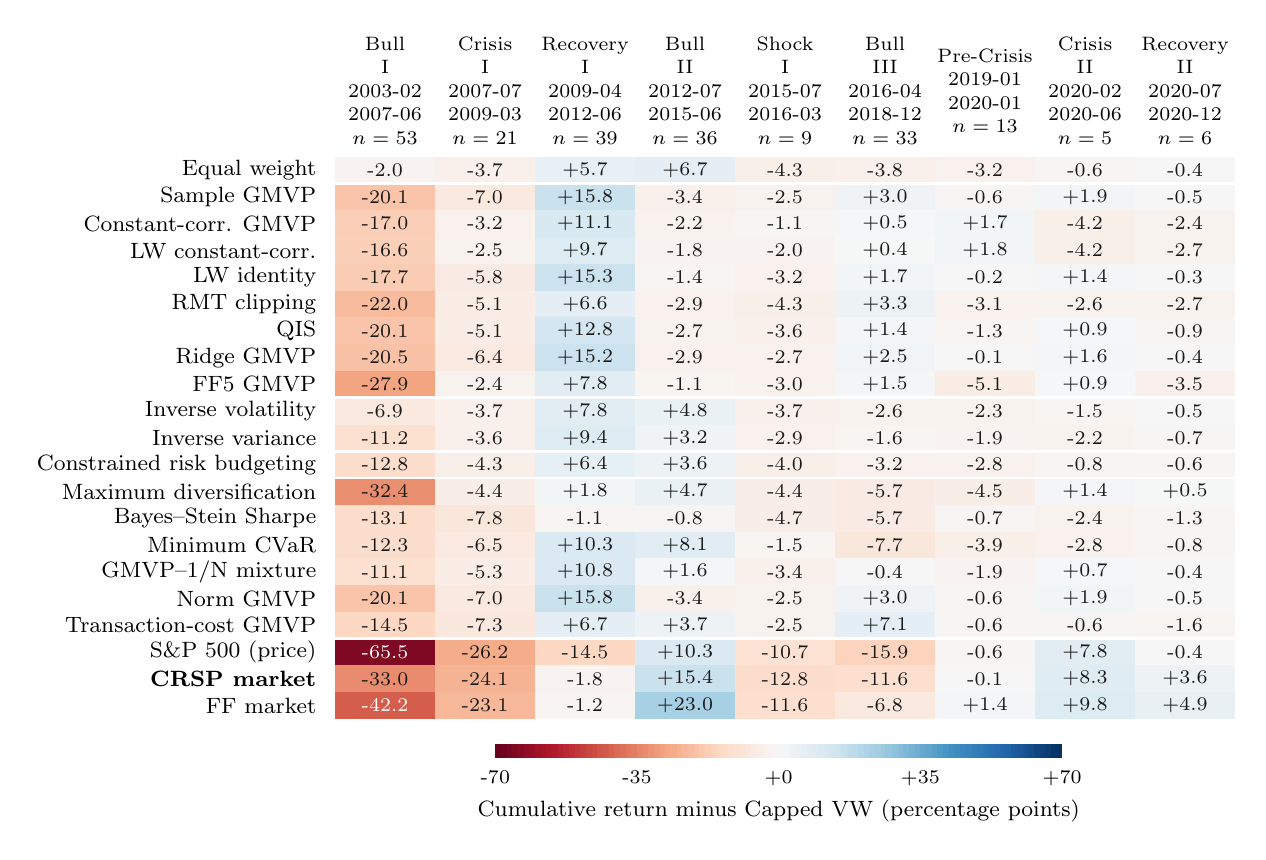
\begin{tikzpicture}[x=1cm,y=1cm]
\node[align=center,font=\fontsize{7.5}{8.5}\selectfont] at (0.000,1.01){Bull\\I\\2003-02\\2007-06\\$n=53$};
\node[align=center,font=\fontsize{7.5}{8.5}\selectfont] at (1.270,1.01){Crisis\\I\\2007-07\\2009-03\\$n=21$};
\node[align=center,font=\fontsize{7.5}{8.5}\selectfont] at (2.540,1.01){Recovery\\I\\2009-04\\2012-06\\$n=39$};
\node[align=center,font=\fontsize{7.5}{8.5}\selectfont] at (3.810,1.01){Bull\\II\\2012-07\\2015-06\\$n=36$};
\node[align=center,font=\fontsize{7.5}{8.5}\selectfont] at (5.080,1.01){Shock\\I\\2015-07\\2016-03\\$n=9$};
\node[align=center,font=\fontsize{7.5}{8.5}\selectfont] at (6.350,1.01){Bull\\III\\2016-04\\2018-12\\$n=33$};
\node[align=center,font=\fontsize{7.5}{8.5}\selectfont] at (7.620,1.01){Pre-Crisis\\2019-01\\2020-01\\$n=13$};
\node[align=center,font=\fontsize{7.5}{8.5}\selectfont] at (8.890,1.01){Crisis\\II\\2020-02\\2020-06\\$n=5$};
\node[align=center,font=\fontsize{7.5}{8.5}\selectfont] at (10.160,1.01){Recovery\\II\\2020-07\\2020-12\\$n=6$};
\node[anchor=east,font=\fontsize{8}{9}\selectfont] at (-0.75,0.000){Equal weight};
\definecolor{cellfill}{HTML}{f8f3f0}
\fill[cellfill] (-0.635,-0.170) rectangle (0.635,0.170);
\node[font=\fontsize{7.5}{8.5}\selectfont,text=black!90] at (0.000,0.000){-2.0};
\definecolor{cellfill}{HTML}{f9f0eb}
\fill[cellfill] (0.635,-0.170) rectangle (1.905,0.170);
\node[font=\fontsize{7.5}{8.5}\selectfont,text=black!90] at (1.270,0.000){-3.7};
\definecolor{cellfill}{HTML}{e7f0f4}
\fill[cellfill] (1.905,-0.170) rectangle (3.175,0.170);
\node[font=\fontsize{7.5}{8.5}\selectfont,text=black!90] at (2.540,0.000){+5.7};
\definecolor{cellfill}{HTML}{e4eef4}
\fill[cellfill] (3.175,-0.170) rectangle (4.445,0.170);
\node[font=\fontsize{7.5}{8.5}\selectfont,text=black!90] at (3.810,0.000){+6.7};
\definecolor{cellfill}{HTML}{f9efe9}
\fill[cellfill] (4.445,-0.170) rectangle (5.715,0.170);
\node[font=\fontsize{7.5}{8.5}\selectfont,text=black!90] at (5.080,0.000){-4.3};
\definecolor{cellfill}{HTML}{f9f0eb}
\fill[cellfill] (5.715,-0.170) rectangle (6.985,0.170);
\node[font=\fontsize{7.5}{8.5}\selectfont,text=black!90] at (6.350,0.000){-3.8};
\definecolor{cellfill}{HTML}{f8f1ed}
\fill[cellfill] (6.985,-0.170) rectangle (8.255,0.170);
\node[font=\fontsize{7.5}{8.5}\selectfont,text=black!90] at (7.620,0.000){-3.2};
\definecolor{cellfill}{HTML}{f7f5f4}
\fill[cellfill] (8.255,-0.170) rectangle (9.525,0.170);
\node[font=\fontsize{7.5}{8.5}\selectfont,text=black!90] at (8.890,0.000){-0.6};
\definecolor{cellfill}{HTML}{f7f6f6}
\fill[cellfill] (9.525,-0.170) rectangle (10.795,0.170);
\node[font=\fontsize{7.5}{8.5}\selectfont,text=black!90] at (10.160,0.000){-0.4};
\node[anchor=east,font=\fontsize{8}{9}\selectfont] at (-0.75,-0.340){Sample GMVP};
\definecolor{cellfill}{HTML}{f9c4a9}
\fill[cellfill] (-0.635,-0.510) rectangle (0.635,-0.170);
\node[font=\fontsize{7.5}{8.5}\selectfont,text=black!90] at (0.000,-0.340){-20.1};
\definecolor{cellfill}{HTML}{fae9df}
\fill[cellfill] (0.635,-0.510) rectangle (1.905,-0.170);
\node[font=\fontsize{7.5}{8.5}\selectfont,text=black!90] at (1.270,-0.340){-7.0};
\definecolor{cellfill}{HTML}{cae1ee}
\fill[cellfill] (1.905,-0.510) rectangle (3.175,-0.170);
\node[font=\fontsize{7.5}{8.5}\selectfont,text=black!90] at (2.540,-0.340){+15.8};
\definecolor{cellfill}{HTML}{f9f0eb}
\fill[cellfill] (3.175,-0.510) rectangle (4.445,-0.170);
\node[font=\fontsize{7.5}{8.5}\selectfont,text=black!90] at (3.810,-0.340){-3.4};
\definecolor{cellfill}{HTML}{f8f2ef}
\fill[cellfill] (4.445,-0.510) rectangle (5.715,-0.170);
\node[font=\fontsize{7.5}{8.5}\selectfont,text=black!90] at (5.080,-0.340){-2.5};
\definecolor{cellfill}{HTML}{eff3f5}
\fill[cellfill] (5.715,-0.510) rectangle (6.985,-0.170);
\node[font=\fontsize{7.5}{8.5}\selectfont,text=black!90] at (6.350,-0.340){+3.0};
\definecolor{cellfill}{HTML}{f7f5f4}
\fill[cellfill] (6.985,-0.510) rectangle (8.255,-0.170);
\node[font=\fontsize{7.5}{8.5}\selectfont,text=black!90] at (7.620,-0.340){-0.6};
\definecolor{cellfill}{HTML}{f2f5f6}
\fill[cellfill] (8.255,-0.510) rectangle (9.525,-0.170);
\node[font=\fontsize{7.5}{8.5}\selectfont,text=black!90] at (8.890,-0.340){+1.9};
\definecolor{cellfill}{HTML}{f7f6f6}
\fill[cellfill] (9.525,-0.510) rectangle (10.795,-0.170);
\node[font=\fontsize{7.5}{8.5}\selectfont,text=black!90] at (10.160,-0.340){-0.5};
\node[anchor=east,font=\fontsize{8}{9}\selectfont] at (-0.75,-0.680){Constant-corr. GMVP};
\definecolor{cellfill}{HTML}{fbceb7}
\fill[cellfill] (-0.635,-0.850) rectangle (0.635,-0.510);
\node[font=\fontsize{7.5}{8.5}\selectfont,text=black!90] at (0.000,-0.680){-17.0};
\definecolor{cellfill}{HTML}{f8f1ed}
\fill[cellfill] (0.635,-0.850) rectangle (1.905,-0.510);
\node[font=\fontsize{7.5}{8.5}\selectfont,text=black!90] at (1.270,-0.680){-3.2};
\definecolor{cellfill}{HTML}{d8e9f1}
\fill[cellfill] (1.905,-0.850) rectangle (3.175,-0.510);
\node[font=\fontsize{7.5}{8.5}\selectfont,text=black!90] at (2.540,-0.680){+11.1};
\definecolor{cellfill}{HTML}{f8f2ef}
\fill[cellfill] (3.175,-0.850) rectangle (4.445,-0.510);
\node[font=\fontsize{7.5}{8.5}\selectfont,text=black!90] at (3.810,-0.680){-2.2};
\definecolor{cellfill}{HTML}{f7f5f4}
\fill[cellfill] (4.445,-0.850) rectangle (5.715,-0.510);
\node[font=\fontsize{7.5}{8.5}\selectfont,text=black!90] at (5.080,-0.680){-1.1};
\definecolor{cellfill}{HTML}{f5f6f7}
\fill[cellfill] (5.715,-0.850) rectangle (6.985,-0.510);
\node[font=\fontsize{7.5}{8.5}\selectfont,text=black!90] at (6.350,-0.680){+0.5};
\definecolor{cellfill}{HTML}{f2f5f6}
\fill[cellfill] (6.985,-0.850) rectangle (8.255,-0.510);
\node[font=\fontsize{7.5}{8.5}\selectfont,text=black!90] at (7.620,-0.680){+1.7};
\definecolor{cellfill}{HTML}{f9efe9}
\fill[cellfill] (8.255,-0.850) rectangle (9.525,-0.510);
\node[font=\fontsize{7.5}{8.5}\selectfont,text=black!90] at (8.890,-0.680){-4.2};
\definecolor{cellfill}{HTML}{f8f2ef}
\fill[cellfill] (9.525,-0.850) rectangle (10.795,-0.510);
\node[font=\fontsize{7.5}{8.5}\selectfont,text=black!90] at (10.160,-0.680){-2.4};
\node[anchor=east,font=\fontsize{8}{9}\selectfont] at (-0.75,-1.020){LW constant-corr.};
\definecolor{cellfill}{HTML}{fbd0b9}
\fill[cellfill] (-0.635,-1.190) rectangle (0.635,-0.850);
\node[font=\fontsize{7.5}{8.5}\selectfont,text=black!90] at (0.000,-1.020){-16.6};
\definecolor{cellfill}{HTML}{f8f2ef}
\fill[cellfill] (0.635,-1.190) rectangle (1.905,-0.850);
\node[font=\fontsize{7.5}{8.5}\selectfont,text=black!90] at (1.270,-1.020){-2.5};
\definecolor{cellfill}{HTML}{ddebf2}
\fill[cellfill] (1.905,-1.190) rectangle (3.175,-0.850);
\node[font=\fontsize{7.5}{8.5}\selectfont,text=black!90] at (2.540,-1.020){+9.7};
\definecolor{cellfill}{HTML}{f8f3f0}
\fill[cellfill] (3.175,-1.190) rectangle (4.445,-0.850);
\node[font=\fontsize{7.5}{8.5}\selectfont,text=black!90] at (3.810,-1.020){-1.8};
\definecolor{cellfill}{HTML}{f8f3f0}
\fill[cellfill] (4.445,-1.190) rectangle (5.715,-0.850);
\node[font=\fontsize{7.5}{8.5}\selectfont,text=black!90] at (5.080,-1.020){-2.0};
\definecolor{cellfill}{HTML}{f6f7f7}
\fill[cellfill] (5.715,-1.190) rectangle (6.985,-0.850);
\node[font=\fontsize{7.5}{8.5}\selectfont,text=black!90] at (6.350,-1.020){+0.4};
\definecolor{cellfill}{HTML}{f2f5f6}
\fill[cellfill] (6.985,-1.190) rectangle (8.255,-0.850);
\node[font=\fontsize{7.5}{8.5}\selectfont,text=black!90] at (7.620,-1.020){+1.8};
\definecolor{cellfill}{HTML}{f9efe9}
\fill[cellfill] (8.255,-1.190) rectangle (9.525,-0.850);
\node[font=\fontsize{7.5}{8.5}\selectfont,text=black!90] at (8.890,-1.020){-4.2};
\definecolor{cellfill}{HTML}{f8f2ef}
\fill[cellfill] (9.525,-1.190) rectangle (10.795,-0.850);
\node[font=\fontsize{7.5}{8.5}\selectfont,text=black!90] at (10.160,-1.020){-2.7};
\node[anchor=east,font=\fontsize{8}{9}\selectfont] at (-0.75,-1.360){LW identity};
\definecolor{cellfill}{HTML}{fbccb4}
\fill[cellfill] (-0.635,-1.530) rectangle (0.635,-1.190);
\node[font=\fontsize{7.5}{8.5}\selectfont,text=black!90] at (0.000,-1.360){-17.7};
\definecolor{cellfill}{HTML}{f9ebe3}
\fill[cellfill] (0.635,-1.530) rectangle (1.905,-1.190);
\node[font=\fontsize{7.5}{8.5}\selectfont,text=black!90] at (1.270,-1.360){-5.8};
\definecolor{cellfill}{HTML}{cce2ef}
\fill[cellfill] (1.905,-1.530) rectangle (3.175,-1.190);
\node[font=\fontsize{7.5}{8.5}\selectfont,text=black!90] at (2.540,-1.360){+15.3};
\definecolor{cellfill}{HTML}{f8f4f2}
\fill[cellfill] (3.175,-1.530) rectangle (4.445,-1.190);
\node[font=\fontsize{7.5}{8.5}\selectfont,text=black!90] at (3.810,-1.360){-1.4};
\definecolor{cellfill}{HTML}{f8f1ed}
\fill[cellfill] (4.445,-1.530) rectangle (5.715,-1.190);
\node[font=\fontsize{7.5}{8.5}\selectfont,text=black!90] at (5.080,-1.360){-3.2};
\definecolor{cellfill}{HTML}{f2f5f6}
\fill[cellfill] (5.715,-1.530) rectangle (6.985,-1.190);
\node[font=\fontsize{7.5}{8.5}\selectfont,text=black!90] at (6.350,-1.360){+1.7};
\definecolor{cellfill}{HTML}{f7f6f6}
\fill[cellfill] (6.985,-1.530) rectangle (8.255,-1.190);
\node[font=\fontsize{7.5}{8.5}\selectfont,text=black!90] at (7.620,-1.360){-0.2};
\definecolor{cellfill}{HTML}{f3f5f6}
\fill[cellfill] (8.255,-1.530) rectangle (9.525,-1.190);
\node[font=\fontsize{7.5}{8.5}\selectfont,text=black!90] at (8.890,-1.360){+1.4};
\definecolor{cellfill}{HTML}{f7f6f6}
\fill[cellfill] (9.525,-1.530) rectangle (10.795,-1.190);
\node[font=\fontsize{7.5}{8.5}\selectfont,text=black!90] at (10.160,-1.360){-0.3};
\node[anchor=east,font=\fontsize{8}{9}\selectfont] at (-0.75,-1.700){RMT clipping};
\definecolor{cellfill}{HTML}{f8bb9e}
\fill[cellfill] (-0.635,-1.870) rectangle (0.635,-1.530);
\node[font=\fontsize{7.5}{8.5}\selectfont,text=black!90] at (0.000,-1.700){-22.0};
\definecolor{cellfill}{HTML}{f9ede5}
\fill[cellfill] (0.635,-1.870) rectangle (1.905,-1.530);
\node[font=\fontsize{7.5}{8.5}\selectfont,text=black!90] at (1.270,-1.700){-5.1};
\definecolor{cellfill}{HTML}{e4eef4}
\fill[cellfill] (1.905,-1.870) rectangle (3.175,-1.530);
\node[font=\fontsize{7.5}{8.5}\selectfont,text=black!90] at (2.540,-1.700){+6.6};
\definecolor{cellfill}{HTML}{f8f1ed}
\fill[cellfill] (3.175,-1.870) rectangle (4.445,-1.530);
\node[font=\fontsize{7.5}{8.5}\selectfont,text=black!90] at (3.810,-1.700){-2.9};
\definecolor{cellfill}{HTML}{f9efe9}
\fill[cellfill] (4.445,-1.870) rectangle (5.715,-1.530);
\node[font=\fontsize{7.5}{8.5}\selectfont,text=black!90] at (5.080,-1.700){-4.3};
\definecolor{cellfill}{HTML}{edf2f5}
\fill[cellfill] (5.715,-1.870) rectangle (6.985,-1.530);
\node[font=\fontsize{7.5}{8.5}\selectfont,text=black!90] at (6.350,-1.700){+3.3};
\definecolor{cellfill}{HTML}{f8f1ed}
\fill[cellfill] (6.985,-1.870) rectangle (8.255,-1.530);
\node[font=\fontsize{7.5}{8.5}\selectfont,text=black!90] at (7.620,-1.700){-3.1};
\definecolor{cellfill}{HTML}{f8f2ef}
\fill[cellfill] (8.255,-1.870) rectangle (9.525,-1.530);
\node[font=\fontsize{7.5}{8.5}\selectfont,text=black!90] at (8.890,-1.700){-2.6};
\definecolor{cellfill}{HTML}{f8f2ef}
\fill[cellfill] (9.525,-1.870) rectangle (10.795,-1.530);
\node[font=\fontsize{7.5}{8.5}\selectfont,text=black!90] at (10.160,-1.700){-2.7};
\node[anchor=east,font=\fontsize{8}{9}\selectfont] at (-0.75,-2.040){QIS};
\definecolor{cellfill}{HTML}{f9c4a9}
\fill[cellfill] (-0.635,-2.210) rectangle (0.635,-1.870);
\node[font=\fontsize{7.5}{8.5}\selectfont,text=black!90] at (0.000,-2.040){-20.1};
\definecolor{cellfill}{HTML}{f9ede5}
\fill[cellfill] (0.635,-2.210) rectangle (1.905,-1.870);
\node[font=\fontsize{7.5}{8.5}\selectfont,text=black!90] at (1.270,-2.040){-5.1};
\definecolor{cellfill}{HTML}{d4e6f1}
\fill[cellfill] (1.905,-2.210) rectangle (3.175,-1.870);
\node[font=\fontsize{7.5}{8.5}\selectfont,text=black!90] at (2.540,-2.040){+12.8};
\definecolor{cellfill}{HTML}{f8f2ef}
\fill[cellfill] (3.175,-2.210) rectangle (4.445,-1.870);
\node[font=\fontsize{7.5}{8.5}\selectfont,text=black!90] at (3.810,-2.040){-2.7};
\definecolor{cellfill}{HTML}{f9f0eb}
\fill[cellfill] (4.445,-2.210) rectangle (5.715,-1.870);
\node[font=\fontsize{7.5}{8.5}\selectfont,text=black!90] at (5.080,-2.040){-3.6};
\definecolor{cellfill}{HTML}{f3f5f6}
\fill[cellfill] (5.715,-2.210) rectangle (6.985,-1.870);
\node[font=\fontsize{7.5}{8.5}\selectfont,text=black!90] at (6.350,-2.040){+1.4};
\definecolor{cellfill}{HTML}{f8f4f2}
\fill[cellfill] (6.985,-2.210) rectangle (8.255,-1.870);
\node[font=\fontsize{7.5}{8.5}\selectfont,text=black!90] at (7.620,-2.040){-1.3};
\definecolor{cellfill}{HTML}{f5f6f7}
\fill[cellfill] (8.255,-2.210) rectangle (9.525,-1.870);
\node[font=\fontsize{7.5}{8.5}\selectfont,text=black!90] at (8.890,-2.040){+0.9};
\definecolor{cellfill}{HTML}{f7f5f4}
\fill[cellfill] (9.525,-2.210) rectangle (10.795,-1.870);
\node[font=\fontsize{7.5}{8.5}\selectfont,text=black!90] at (10.160,-2.040){-0.9};
\node[anchor=east,font=\fontsize{8}{9}\selectfont] at (-0.75,-2.380){Ridge GMVP};
\definecolor{cellfill}{HTML}{f9c2a7}
\fill[cellfill] (-0.635,-2.550) rectangle (0.635,-2.210);
\node[font=\fontsize{7.5}{8.5}\selectfont,text=black!90] at (0.000,-2.380){-20.5};
\definecolor{cellfill}{HTML}{faeae1}
\fill[cellfill] (0.635,-2.550) rectangle (1.905,-2.210);
\node[font=\fontsize{7.5}{8.5}\selectfont,text=black!90] at (1.270,-2.380){-6.4};
\definecolor{cellfill}{HTML}{cce2ef}
\fill[cellfill] (1.905,-2.550) rectangle (3.175,-2.210);
\node[font=\fontsize{7.5}{8.5}\selectfont,text=black!90] at (2.540,-2.380){+15.2};
\definecolor{cellfill}{HTML}{f8f1ed}
\fill[cellfill] (3.175,-2.550) rectangle (4.445,-2.210);
\node[font=\fontsize{7.5}{8.5}\selectfont,text=black!90] at (3.810,-2.380){-2.9};
\definecolor{cellfill}{HTML}{f8f1ed}
\fill[cellfill] (4.445,-2.550) rectangle (5.715,-2.210);
\node[font=\fontsize{7.5}{8.5}\selectfont,text=black!90] at (5.080,-2.380){-2.7};
\definecolor{cellfill}{HTML}{f0f4f6}
\fill[cellfill] (5.715,-2.550) rectangle (6.985,-2.210);
\node[font=\fontsize{7.5}{8.5}\selectfont,text=black!90] at (6.350,-2.380){+2.5};
\definecolor{cellfill}{HTML}{f7f6f6}
\fill[cellfill] (6.985,-2.550) rectangle (8.255,-2.210);
\node[font=\fontsize{7.5}{8.5}\selectfont,text=black!90] at (7.620,-2.380){-0.1};
\definecolor{cellfill}{HTML}{f3f5f6}
\fill[cellfill] (8.255,-2.550) rectangle (9.525,-2.210);
\node[font=\fontsize{7.5}{8.5}\selectfont,text=black!90] at (8.890,-2.380){+1.6};
\definecolor{cellfill}{HTML}{f7f6f6}
\fill[cellfill] (9.525,-2.550) rectangle (10.795,-2.210);
\node[font=\fontsize{7.5}{8.5}\selectfont,text=black!90] at (10.160,-2.380){-0.4};
\node[anchor=east,font=\fontsize{8}{9}\selectfont] at (-0.75,-2.720){FF5 GMVP};
\definecolor{cellfill}{HTML}{f3a481}
\fill[cellfill] (-0.635,-2.890) rectangle (0.635,-2.550);
\node[font=\fontsize{7.5}{8.5}\selectfont,text=black!90] at (0.000,-2.720){-27.9};
\definecolor{cellfill}{HTML}{f8f2ef}
\fill[cellfill] (0.635,-2.890) rectangle (1.905,-2.550);
\node[font=\fontsize{7.5}{8.5}\selectfont,text=black!90] at (1.270,-2.720){-2.4};
\definecolor{cellfill}{HTML}{e1edf3}
\fill[cellfill] (1.905,-2.890) rectangle (3.175,-2.550);
\node[font=\fontsize{7.5}{8.5}\selectfont,text=black!90] at (2.540,-2.720){+7.8};
\definecolor{cellfill}{HTML}{f8f4f2}
\fill[cellfill] (3.175,-2.890) rectangle (4.445,-2.550);
\node[font=\fontsize{7.5}{8.5}\selectfont,text=black!90] at (3.810,-2.720){-1.1};
\definecolor{cellfill}{HTML}{f8f1ed}
\fill[cellfill] (4.445,-2.890) rectangle (5.715,-2.550);
\node[font=\fontsize{7.5}{8.5}\selectfont,text=black!90] at (5.080,-2.720){-3.0};
\definecolor{cellfill}{HTML}{f3f5f6}
\fill[cellfill] (5.715,-2.890) rectangle (6.985,-2.550);
\node[font=\fontsize{7.5}{8.5}\selectfont,text=black!90] at (6.350,-2.720){+1.5};
\definecolor{cellfill}{HTML}{f9ede5}
\fill[cellfill] (6.985,-2.890) rectangle (8.255,-2.550);
\node[font=\fontsize{7.5}{8.5}\selectfont,text=black!90] at (7.620,-2.720){-5.1};
\definecolor{cellfill}{HTML}{f5f6f7}
\fill[cellfill] (8.255,-2.890) rectangle (9.525,-2.550);
\node[font=\fontsize{7.5}{8.5}\selectfont,text=black!90] at (8.890,-2.720){+0.9};
\definecolor{cellfill}{HTML}{f9f0eb}
\fill[cellfill] (9.525,-2.890) rectangle (10.795,-2.550);
\node[font=\fontsize{7.5}{8.5}\selectfont,text=black!90] at (10.160,-2.720){-3.5};
\node[anchor=east,font=\fontsize{8}{9}\selectfont] at (-0.75,-3.060){Inverse volatility};
\definecolor{cellfill}{HTML}{fae9df}
\fill[cellfill] (-0.635,-3.230) rectangle (0.635,-2.890);
\node[font=\fontsize{7.5}{8.5}\selectfont,text=black!90] at (0.000,-3.060){-6.9};
\definecolor{cellfill}{HTML}{f9f0eb}
\fill[cellfill] (0.635,-3.230) rectangle (1.905,-2.890);
\node[font=\fontsize{7.5}{8.5}\selectfont,text=black!90] at (1.270,-3.060){-3.7};
\definecolor{cellfill}{HTML}{e1edf3}
\fill[cellfill] (1.905,-3.230) rectangle (3.175,-2.890);
\node[font=\fontsize{7.5}{8.5}\selectfont,text=black!90] at (2.540,-3.060){+7.8};
\definecolor{cellfill}{HTML}{eaf1f5}
\fill[cellfill] (3.175,-3.230) rectangle (4.445,-2.890);
\node[font=\fontsize{7.5}{8.5}\selectfont,text=black!90] at (3.810,-3.060){+4.8};
\definecolor{cellfill}{HTML}{f9f0eb}
\fill[cellfill] (4.445,-3.230) rectangle (5.715,-2.890);
\node[font=\fontsize{7.5}{8.5}\selectfont,text=black!90] at (5.080,-3.060){-3.7};
\definecolor{cellfill}{HTML}{f8f2ef}
\fill[cellfill] (5.715,-3.230) rectangle (6.985,-2.890);
\node[font=\fontsize{7.5}{8.5}\selectfont,text=black!90] at (6.350,-3.060){-2.6};
\definecolor{cellfill}{HTML}{f8f2ef}
\fill[cellfill] (6.985,-3.230) rectangle (8.255,-2.890);
\node[font=\fontsize{7.5}{8.5}\selectfont,text=black!90] at (7.620,-3.060){-2.3};
\definecolor{cellfill}{HTML}{f8f4f2}
\fill[cellfill] (8.255,-3.230) rectangle (9.525,-2.890);
\node[font=\fontsize{7.5}{8.5}\selectfont,text=black!90] at (8.890,-3.060){-1.5};
\definecolor{cellfill}{HTML}{f7f6f6}
\fill[cellfill] (9.525,-3.230) rectangle (10.795,-2.890);
\node[font=\fontsize{7.5}{8.5}\selectfont,text=black!90] at (10.160,-3.060){-0.5};
\node[anchor=east,font=\fontsize{8}{9}\selectfont] at (-0.75,-3.400){Inverse variance};
\definecolor{cellfill}{HTML}{fce0d0}
\fill[cellfill] (-0.635,-3.570) rectangle (0.635,-3.230);
\node[font=\fontsize{7.5}{8.5}\selectfont,text=black!90] at (0.000,-3.400){-11.2};
\definecolor{cellfill}{HTML}{f9f0eb}
\fill[cellfill] (0.635,-3.570) rectangle (1.905,-3.230);
\node[font=\fontsize{7.5}{8.5}\selectfont,text=black!90] at (1.270,-3.400){-3.6};
\definecolor{cellfill}{HTML}{ddebf2}
\fill[cellfill] (1.905,-3.570) rectangle (3.175,-3.230);
\node[font=\fontsize{7.5}{8.5}\selectfont,text=black!90] at (2.540,-3.400){+9.4};
\definecolor{cellfill}{HTML}{eff3f5}
\fill[cellfill] (3.175,-3.570) rectangle (4.445,-3.230);
\node[font=\fontsize{7.5}{8.5}\selectfont,text=black!90] at (3.810,-3.400){+3.2};
\definecolor{cellfill}{HTML}{f8f1ed}
\fill[cellfill] (4.445,-3.570) rectangle (5.715,-3.230);
\node[font=\fontsize{7.5}{8.5}\selectfont,text=black!90] at (5.080,-3.400){-2.9};
\definecolor{cellfill}{HTML}{f8f4f2}
\fill[cellfill] (5.715,-3.570) rectangle (6.985,-3.230);
\node[font=\fontsize{7.5}{8.5}\selectfont,text=black!90] at (6.350,-3.400){-1.6};
\definecolor{cellfill}{HTML}{f8f3f0}
\fill[cellfill] (6.985,-3.570) rectangle (8.255,-3.230);
\node[font=\fontsize{7.5}{8.5}\selectfont,text=black!90] at (7.620,-3.400){-1.9};
\definecolor{cellfill}{HTML}{f8f2ef}
\fill[cellfill] (8.255,-3.570) rectangle (9.525,-3.230);
\node[font=\fontsize{7.5}{8.5}\selectfont,text=black!90] at (8.890,-3.400){-2.2};
\definecolor{cellfill}{HTML}{f7f5f4}
\fill[cellfill] (9.525,-3.570) rectangle (10.795,-3.230);
\node[font=\fontsize{7.5}{8.5}\selectfont,text=black!90] at (10.160,-3.400){-0.7};
\node[anchor=east,font=\fontsize{8}{9}\selectfont] at (-0.75,-3.740){Constrained risk budgeting};
\definecolor{cellfill}{HTML}{fdddcb}
\fill[cellfill] (-0.635,-3.910) rectangle (0.635,-3.570);
\node[font=\fontsize{7.5}{8.5}\selectfont,text=black!90] at (0.000,-3.740){-12.8};
\definecolor{cellfill}{HTML}{f9efe9}
\fill[cellfill] (0.635,-3.910) rectangle (1.905,-3.570);
\node[font=\fontsize{7.5}{8.5}\selectfont,text=black!90] at (1.270,-3.740){-4.3};
\definecolor{cellfill}{HTML}{e6eff4}
\fill[cellfill] (1.905,-3.910) rectangle (3.175,-3.570);
\node[font=\fontsize{7.5}{8.5}\selectfont,text=black!90] at (2.540,-3.740){+6.4};
\definecolor{cellfill}{HTML}{edf2f5}
\fill[cellfill] (3.175,-3.910) rectangle (4.445,-3.570);
\node[font=\fontsize{7.5}{8.5}\selectfont,text=black!90] at (3.810,-3.740){+3.6};
\definecolor{cellfill}{HTML}{f9efe9}
\fill[cellfill] (4.445,-3.910) rectangle (5.715,-3.570);
\node[font=\fontsize{7.5}{8.5}\selectfont,text=black!90] at (5.080,-3.740){-4.0};
\definecolor{cellfill}{HTML}{f8f1ed}
\fill[cellfill] (5.715,-3.910) rectangle (6.985,-3.570);
\node[font=\fontsize{7.5}{8.5}\selectfont,text=black!90] at (6.350,-3.740){-3.2};
\definecolor{cellfill}{HTML}{f8f1ed}
\fill[cellfill] (6.985,-3.910) rectangle (8.255,-3.570);
\node[font=\fontsize{7.5}{8.5}\selectfont,text=black!90] at (7.620,-3.740){-2.8};
\definecolor{cellfill}{HTML}{f7f5f4}
\fill[cellfill] (8.255,-3.910) rectangle (9.525,-3.570);
\node[font=\fontsize{7.5}{8.5}\selectfont,text=black!90] at (8.890,-3.740){-0.8};
\definecolor{cellfill}{HTML}{f7f5f4}
\fill[cellfill] (9.525,-3.910) rectangle (10.795,-3.570);
\node[font=\fontsize{7.5}{8.5}\selectfont,text=black!90] at (10.160,-3.740){-0.6};
\node[anchor=east,font=\fontsize{8}{9}\selectfont] at (-0.75,-4.080){Maximum diversification};
\definecolor{cellfill}{HTML}{ea8e70}
\fill[cellfill] (-0.635,-4.250) rectangle (0.635,-3.910);
\node[font=\fontsize{7.5}{8.5}\selectfont,text=black!90] at (0.000,-4.080){-32.4};
\definecolor{cellfill}{HTML}{f9eee7}
\fill[cellfill] (0.635,-4.250) rectangle (1.905,-3.910);
\node[font=\fontsize{7.5}{8.5}\selectfont,text=black!90] at (1.270,-4.080){-4.4};
\definecolor{cellfill}{HTML}{f2f5f6}
\fill[cellfill] (1.905,-4.250) rectangle (3.175,-3.910);
\node[font=\fontsize{7.5}{8.5}\selectfont,text=black!90] at (2.540,-4.080){+1.8};
\definecolor{cellfill}{HTML}{eaf1f5}
\fill[cellfill] (3.175,-4.250) rectangle (4.445,-3.910);
\node[font=\fontsize{7.5}{8.5}\selectfont,text=black!90] at (3.810,-4.080){+4.7};
\definecolor{cellfill}{HTML}{f9eee7}
\fill[cellfill] (4.445,-4.250) rectangle (5.715,-3.910);
\node[font=\fontsize{7.5}{8.5}\selectfont,text=black!90] at (5.080,-4.080){-4.4};
\definecolor{cellfill}{HTML}{f9ebe3}
\fill[cellfill] (5.715,-4.250) rectangle (6.985,-3.910);
\node[font=\fontsize{7.5}{8.5}\selectfont,text=black!90] at (6.350,-4.080){-5.7};
\definecolor{cellfill}{HTML}{f9eee7}
\fill[cellfill] (6.985,-4.250) rectangle (8.255,-3.910);
\node[font=\fontsize{7.5}{8.5}\selectfont,text=black!90] at (7.620,-4.080){-4.5};
\definecolor{cellfill}{HTML}{f3f5f6}
\fill[cellfill] (8.255,-4.250) rectangle (9.525,-3.910);
\node[font=\fontsize{7.5}{8.5}\selectfont,text=black!90] at (8.890,-4.080){+1.4};
\definecolor{cellfill}{HTML}{f6f7f7}
\fill[cellfill] (9.525,-4.250) rectangle (10.795,-3.910);
\node[font=\fontsize{7.5}{8.5}\selectfont,text=black!90] at (10.160,-4.080){+0.5};
\node[anchor=east,font=\fontsize{8}{9}\selectfont] at (-0.75,-4.420){Bayes--Stein Sharpe};
\definecolor{cellfill}{HTML}{fdddcb}
\fill[cellfill] (-0.635,-4.590) rectangle (0.635,-4.250);
\node[font=\fontsize{7.5}{8.5}\selectfont,text=black!90] at (0.000,-4.420){-13.1};
\definecolor{cellfill}{HTML}{fae7dc}
\fill[cellfill] (0.635,-4.590) rectangle (1.905,-4.250);
\node[font=\fontsize{7.5}{8.5}\selectfont,text=black!90] at (1.270,-4.420){-7.8};
\definecolor{cellfill}{HTML}{f8f4f2}
\fill[cellfill] (1.905,-4.590) rectangle (3.175,-4.250);
\node[font=\fontsize{7.5}{8.5}\selectfont,text=black!90] at (2.540,-4.420){-1.1};
\definecolor{cellfill}{HTML}{f7f5f4}
\fill[cellfill] (3.175,-4.590) rectangle (4.445,-4.250);
\node[font=\fontsize{7.5}{8.5}\selectfont,text=black!90] at (3.810,-4.420){-0.8};
\definecolor{cellfill}{HTML}{f9eee7}
\fill[cellfill] (4.445,-4.590) rectangle (5.715,-4.250);
\node[font=\fontsize{7.5}{8.5}\selectfont,text=black!90] at (5.080,-4.420){-4.7};
\definecolor{cellfill}{HTML}{f9ebe3}
\fill[cellfill] (5.715,-4.590) rectangle (6.985,-4.250);
\node[font=\fontsize{7.5}{8.5}\selectfont,text=black!90] at (6.350,-4.420){-5.7};
\definecolor{cellfill}{HTML}{f7f5f4}
\fill[cellfill] (6.985,-4.590) rectangle (8.255,-4.250);
\node[font=\fontsize{7.5}{8.5}\selectfont,text=black!90] at (7.620,-4.420){-0.7};
\definecolor{cellfill}{HTML}{f8f2ef}
\fill[cellfill] (8.255,-4.590) rectangle (9.525,-4.250);
\node[font=\fontsize{7.5}{8.5}\selectfont,text=black!90] at (8.890,-4.420){-2.4};
\definecolor{cellfill}{HTML}{f8f4f2}
\fill[cellfill] (9.525,-4.590) rectangle (10.795,-4.250);
\node[font=\fontsize{7.5}{8.5}\selectfont,text=black!90] at (10.160,-4.420){-1.3};
\node[anchor=east,font=\fontsize{8}{9}\selectfont] at (-0.75,-4.760){Minimum CVaR};
\definecolor{cellfill}{HTML}{fcdecd}
\fill[cellfill] (-0.635,-4.930) rectangle (0.635,-4.590);
\node[font=\fontsize{7.5}{8.5}\selectfont,text=black!90] at (0.000,-4.760){-12.3};
\definecolor{cellfill}{HTML}{faeae1}
\fill[cellfill] (0.635,-4.930) rectangle (1.905,-4.590);
\node[font=\fontsize{7.5}{8.5}\selectfont,text=black!90] at (1.270,-4.760){-6.5};
\definecolor{cellfill}{HTML}{dbeaf2}
\fill[cellfill] (1.905,-4.930) rectangle (3.175,-4.590);
\node[font=\fontsize{7.5}{8.5}\selectfont,text=black!90] at (2.540,-4.760){+10.3};
\definecolor{cellfill}{HTML}{e1edf3}
\fill[cellfill] (3.175,-4.930) rectangle (4.445,-4.590);
\node[font=\fontsize{7.5}{8.5}\selectfont,text=black!90] at (3.810,-4.760){+8.1};
\definecolor{cellfill}{HTML}{f8f4f2}
\fill[cellfill] (4.445,-4.930) rectangle (5.715,-4.590);
\node[font=\fontsize{7.5}{8.5}\selectfont,text=black!90] at (5.080,-4.760){-1.5};
\definecolor{cellfill}{HTML}{fae7dc}
\fill[cellfill] (5.715,-4.930) rectangle (6.985,-4.590);
\node[font=\fontsize{7.5}{8.5}\selectfont,text=black!90] at (6.350,-4.760){-7.7};
\definecolor{cellfill}{HTML}{f9efe9}
\fill[cellfill] (6.985,-4.930) rectangle (8.255,-4.590);
\node[font=\fontsize{7.5}{8.5}\selectfont,text=black!90] at (7.620,-4.760){-3.9};
\definecolor{cellfill}{HTML}{f8f1ed}
\fill[cellfill] (8.255,-4.930) rectangle (9.525,-4.590);
\node[font=\fontsize{7.5}{8.5}\selectfont,text=black!90] at (8.890,-4.760){-2.8};
\definecolor{cellfill}{HTML}{f7f5f4}
\fill[cellfill] (9.525,-4.930) rectangle (10.795,-4.590);
\node[font=\fontsize{7.5}{8.5}\selectfont,text=black!90] at (10.160,-4.760){-0.8};
\node[anchor=east,font=\fontsize{8}{9}\selectfont] at (-0.75,-5.100){GMVP--1/N mixture};
\definecolor{cellfill}{HTML}{fce0d0}
\fill[cellfill] (-0.635,-5.270) rectangle (0.635,-4.930);
\node[font=\fontsize{7.5}{8.5}\selectfont,text=black!90] at (0.000,-5.100){-11.1};
\definecolor{cellfill}{HTML}{f9ede5}
\fill[cellfill] (0.635,-5.270) rectangle (1.905,-4.930);
\node[font=\fontsize{7.5}{8.5}\selectfont,text=black!90] at (1.270,-5.100){-5.3};
\definecolor{cellfill}{HTML}{dae9f2}
\fill[cellfill] (1.905,-5.270) rectangle (3.175,-4.930);
\node[font=\fontsize{7.5}{8.5}\selectfont,text=black!90] at (2.540,-5.100){+10.8};
\definecolor{cellfill}{HTML}{f3f5f6}
\fill[cellfill] (3.175,-5.270) rectangle (4.445,-4.930);
\node[font=\fontsize{7.5}{8.5}\selectfont,text=black!90] at (3.810,-5.100){+1.6};
\definecolor{cellfill}{HTML}{f9f0eb}
\fill[cellfill] (4.445,-5.270) rectangle (5.715,-4.930);
\node[font=\fontsize{7.5}{8.5}\selectfont,text=black!90] at (5.080,-5.100){-3.4};
\definecolor{cellfill}{HTML}{f7f6f6}
\fill[cellfill] (5.715,-5.270) rectangle (6.985,-4.930);
\node[font=\fontsize{7.5}{8.5}\selectfont,text=black!90] at (6.350,-5.100){-0.4};
\definecolor{cellfill}{HTML}{f8f3f0}
\fill[cellfill] (6.985,-5.270) rectangle (8.255,-4.930);
\node[font=\fontsize{7.5}{8.5}\selectfont,text=black!90] at (7.620,-5.100){-1.9};
\definecolor{cellfill}{HTML}{f5f6f7}
\fill[cellfill] (8.255,-5.270) rectangle (9.525,-4.930);
\node[font=\fontsize{7.5}{8.5}\selectfont,text=black!90] at (8.890,-5.100){+0.7};
\definecolor{cellfill}{HTML}{f7f6f6}
\fill[cellfill] (9.525,-5.270) rectangle (10.795,-4.930);
\node[font=\fontsize{7.5}{8.5}\selectfont,text=black!90] at (10.160,-5.100){-0.4};
\node[anchor=east,font=\fontsize{8}{9}\selectfont] at (-0.75,-5.440){Norm GMVP};
\definecolor{cellfill}{HTML}{f9c4a9}
\fill[cellfill] (-0.635,-5.610) rectangle (0.635,-5.270);
\node[font=\fontsize{7.5}{8.5}\selectfont,text=black!90] at (0.000,-5.440){-20.1};
\definecolor{cellfill}{HTML}{fae9df}
\fill[cellfill] (0.635,-5.610) rectangle (1.905,-5.270);
\node[font=\fontsize{7.5}{8.5}\selectfont,text=black!90] at (1.270,-5.440){-7.0};
\definecolor{cellfill}{HTML}{cae1ee}
\fill[cellfill] (1.905,-5.610) rectangle (3.175,-5.270);
\node[font=\fontsize{7.5}{8.5}\selectfont,text=black!90] at (2.540,-5.440){+15.8};
\definecolor{cellfill}{HTML}{f9f0eb}
\fill[cellfill] (3.175,-5.610) rectangle (4.445,-5.270);
\node[font=\fontsize{7.5}{8.5}\selectfont,text=black!90] at (3.810,-5.440){-3.4};
\definecolor{cellfill}{HTML}{f8f2ef}
\fill[cellfill] (4.445,-5.610) rectangle (5.715,-5.270);
\node[font=\fontsize{7.5}{8.5}\selectfont,text=black!90] at (5.080,-5.440){-2.5};
\definecolor{cellfill}{HTML}{eff3f5}
\fill[cellfill] (5.715,-5.610) rectangle (6.985,-5.270);
\node[font=\fontsize{7.5}{8.5}\selectfont,text=black!90] at (6.350,-5.440){+3.0};
\definecolor{cellfill}{HTML}{f7f5f4}
\fill[cellfill] (6.985,-5.610) rectangle (8.255,-5.270);
\node[font=\fontsize{7.5}{8.5}\selectfont,text=black!90] at (7.620,-5.440){-0.6};
\definecolor{cellfill}{HTML}{f2f5f6}
\fill[cellfill] (8.255,-5.610) rectangle (9.525,-5.270);
\node[font=\fontsize{7.5}{8.5}\selectfont,text=black!90] at (8.890,-5.440){+1.9};
\definecolor{cellfill}{HTML}{f7f6f6}
\fill[cellfill] (9.525,-5.610) rectangle (10.795,-5.270);
\node[font=\fontsize{7.5}{8.5}\selectfont,text=black!90] at (10.160,-5.440){-0.5};
\node[anchor=east,font=\fontsize{8}{9}\selectfont] at (-0.75,-5.780){Transaction-cost GMVP};
\definecolor{cellfill}{HTML}{fdd9c4}
\fill[cellfill] (-0.635,-5.950) rectangle (0.635,-5.610);
\node[font=\fontsize{7.5}{8.5}\selectfont,text=black!90] at (0.000,-5.780){-14.5};
\definecolor{cellfill}{HTML}{fae8de}
\fill[cellfill] (0.635,-5.950) rectangle (1.905,-5.610);
\node[font=\fontsize{7.5}{8.5}\selectfont,text=black!90] at (1.270,-5.780){-7.3};
\definecolor{cellfill}{HTML}{e4eef4}
\fill[cellfill] (1.905,-5.950) rectangle (3.175,-5.610);
\node[font=\fontsize{7.5}{8.5}\selectfont,text=black!90] at (2.540,-5.780){+6.7};
\definecolor{cellfill}{HTML}{edf2f5}
\fill[cellfill] (3.175,-5.950) rectangle (4.445,-5.610);
\node[font=\fontsize{7.5}{8.5}\selectfont,text=black!90] at (3.810,-5.780){+3.7};
\definecolor{cellfill}{HTML}{f8f2ef}
\fill[cellfill] (4.445,-5.950) rectangle (5.715,-5.610);
\node[font=\fontsize{7.5}{8.5}\selectfont,text=black!90] at (5.080,-5.780){-2.5};
\definecolor{cellfill}{HTML}{e4eef4}
\fill[cellfill] (5.715,-5.950) rectangle (6.985,-5.610);
\node[font=\fontsize{7.5}{8.5}\selectfont,text=black!90] at (6.350,-5.780){+7.1};
\definecolor{cellfill}{HTML}{f7f5f4}
\fill[cellfill] (6.985,-5.950) rectangle (8.255,-5.610);
\node[font=\fontsize{7.5}{8.5}\selectfont,text=black!90] at (7.620,-5.780){-0.6};
\definecolor{cellfill}{HTML}{f7f5f4}
\fill[cellfill] (8.255,-5.950) rectangle (9.525,-5.610);
\node[font=\fontsize{7.5}{8.5}\selectfont,text=black!90] at (8.890,-5.780){-0.6};
\definecolor{cellfill}{HTML}{f8f4f2}
\fill[cellfill] (9.525,-5.950) rectangle (10.795,-5.610);
\node[font=\fontsize{7.5}{8.5}\selectfont,text=black!90] at (10.160,-5.780){-1.6};
\node[anchor=east,font=\fontsize{8}{9}\selectfont] at (-0.75,-6.120){S\&P 500 (price)};
\definecolor{cellfill}{HTML}{7f0823}
\fill[cellfill] (-0.635,-6.290) rectangle (0.635,-5.950);
\node[font=\fontsize{7.5}{8.5}\selectfont,text=white] at (0.000,-6.120){-65.5};
\definecolor{cellfill}{HTML}{f5ac8b}
\fill[cellfill] (0.635,-6.290) rectangle (1.905,-5.950);
\node[font=\fontsize{7.5}{8.5}\selectfont,text=black!90] at (1.270,-6.120){-26.2};
\definecolor{cellfill}{HTML}{fdd9c4}
\fill[cellfill] (1.905,-6.290) rectangle (3.175,-5.950);
\node[font=\fontsize{7.5}{8.5}\selectfont,text=black!90] at (2.540,-6.120){-14.5};
\definecolor{cellfill}{HTML}{dbeaf2}
\fill[cellfill] (3.175,-6.290) rectangle (4.445,-5.950);
\node[font=\fontsize{7.5}{8.5}\selectfont,text=black!90] at (3.810,-6.120){+10.3};
\definecolor{cellfill}{HTML}{fce2d2}
\fill[cellfill] (4.445,-6.290) rectangle (5.715,-5.950);
\node[font=\fontsize{7.5}{8.5}\selectfont,text=black!90] at (5.080,-6.120){-10.7};
\definecolor{cellfill}{HTML}{fcd3bc}
\fill[cellfill] (5.715,-6.290) rectangle (6.985,-5.950);
\node[font=\fontsize{7.5}{8.5}\selectfont,text=black!90] at (6.350,-6.120){-15.9};
\definecolor{cellfill}{HTML}{f7f5f4}
\fill[cellfill] (6.985,-6.290) rectangle (8.255,-5.950);
\node[font=\fontsize{7.5}{8.5}\selectfont,text=black!90] at (7.620,-6.120){-0.6};
\definecolor{cellfill}{HTML}{e1edf3}
\fill[cellfill] (8.255,-6.290) rectangle (9.525,-5.950);
\node[font=\fontsize{7.5}{8.5}\selectfont,text=black!90] at (8.890,-6.120){+7.8};
\definecolor{cellfill}{HTML}{f7f6f6}
\fill[cellfill] (9.525,-6.290) rectangle (10.795,-5.950);
\node[font=\fontsize{7.5}{8.5}\selectfont,text=black!90] at (10.160,-6.120){-0.4};
\node[anchor=east,font=\fontsize{8}{9}\selectfont] at (-0.75,-6.460){\textbf{CRSP market}};
\definecolor{cellfill}{HTML}{e98b6e}
\fill[cellfill] (-0.635,-6.630) rectangle (0.635,-6.290);
\node[font=\fontsize{7.5}{8.5}\selectfont,text=black!90] at (0.000,-6.460){-33.0};
\definecolor{cellfill}{HTML}{f6b394}
\fill[cellfill] (0.635,-6.630) rectangle (1.905,-6.290);
\node[font=\fontsize{7.5}{8.5}\selectfont,text=black!90] at (1.270,-6.460){-24.1};
\definecolor{cellfill}{HTML}{f8f3f0}
\fill[cellfill] (1.905,-6.630) rectangle (3.175,-6.290);
\node[font=\fontsize{7.5}{8.5}\selectfont,text=black!90] at (2.540,-6.460){-1.8};
\definecolor{cellfill}{HTML}{cae1ee}
\fill[cellfill] (3.175,-6.630) rectangle (4.445,-6.290);
\node[font=\fontsize{7.5}{8.5}\selectfont,text=black!90] at (3.810,-6.460){+15.4};
\definecolor{cellfill}{HTML}{fdddcb}
\fill[cellfill] (4.445,-6.630) rectangle (5.715,-6.290);
\node[font=\fontsize{7.5}{8.5}\selectfont,text=black!90] at (5.080,-6.460){-12.8};
\definecolor{cellfill}{HTML}{fcdfcf}
\fill[cellfill] (5.715,-6.630) rectangle (6.985,-6.290);
\node[font=\fontsize{7.5}{8.5}\selectfont,text=black!90] at (6.350,-6.460){-11.6};
\definecolor{cellfill}{HTML}{f7f6f6}
\fill[cellfill] (6.985,-6.630) rectangle (8.255,-6.290);
\node[font=\fontsize{7.5}{8.5}\selectfont,text=black!90] at (7.620,-6.460){-0.1};
\definecolor{cellfill}{HTML}{e0ecf3}
\fill[cellfill] (8.255,-6.630) rectangle (9.525,-6.290);
\node[font=\fontsize{7.5}{8.5}\selectfont,text=black!90] at (8.890,-6.460){+8.3};
\definecolor{cellfill}{HTML}{edf2f5}
\fill[cellfill] (9.525,-6.630) rectangle (10.795,-6.290);
\node[font=\fontsize{7.5}{8.5}\selectfont,text=black!90] at (10.160,-6.460){+3.6};
\node[anchor=east,font=\fontsize{8}{9}\selectfont] at (-0.75,-6.800){FF market};
\definecolor{cellfill}{HTML}{d55d4c}
\fill[cellfill] (-0.635,-6.970) rectangle (0.635,-6.630);
\node[font=\fontsize{7.5}{8.5}\selectfont,text=white] at (0.000,-6.800){-42.2};
\definecolor{cellfill}{HTML}{f7b799}
\fill[cellfill] (0.635,-6.970) rectangle (1.905,-6.630);
\node[font=\fontsize{7.5}{8.5}\selectfont,text=black!90] at (1.270,-6.800){-23.1};
\definecolor{cellfill}{HTML}{f8f4f2}
\fill[cellfill] (1.905,-6.970) rectangle (3.175,-6.630);
\node[font=\fontsize{7.5}{8.5}\selectfont,text=black!90] at (2.540,-6.800){-1.2};
\definecolor{cellfill}{HTML}{a7d0e4}
\fill[cellfill] (3.175,-6.970) rectangle (4.445,-6.630);
\node[font=\fontsize{7.5}{8.5}\selectfont,text=black!90] at (3.810,-6.800){+23.0};
\definecolor{cellfill}{HTML}{fcdfcf}
\fill[cellfill] (4.445,-6.970) rectangle (5.715,-6.630);
\node[font=\fontsize{7.5}{8.5}\selectfont,text=black!90] at (5.080,-6.800){-11.6};
\definecolor{cellfill}{HTML}{fae9df}
\fill[cellfill] (5.715,-6.970) rectangle (6.985,-6.630);
\node[font=\fontsize{7.5}{8.5}\selectfont,text=black!90] at (6.350,-6.800){-6.8};
\definecolor{cellfill}{HTML}{f3f5f6}
\fill[cellfill] (6.985,-6.970) rectangle (8.255,-6.630);
\node[font=\fontsize{7.5}{8.5}\selectfont,text=black!90] at (7.620,-6.800){+1.4};
\definecolor{cellfill}{HTML}{ddebf2}
\fill[cellfill] (8.255,-6.970) rectangle (9.525,-6.630);
\node[font=\fontsize{7.5}{8.5}\selectfont,text=black!90] at (8.890,-6.800){+9.8};
\definecolor{cellfill}{HTML}{e9f0f4}
\fill[cellfill] (9.525,-6.970) rectangle (10.795,-6.630);
\node[font=\fontsize{7.5}{8.5}\selectfont,text=black!90] at (10.160,-6.800){+4.9};
\draw[white,line width=1pt] (-0.635,-0.170)--(10.795,-0.170);
\draw[white,line width=1pt] (-0.635,-2.890)--(10.795,-2.890);
\draw[white,line width=1pt] (-0.635,-3.570)--(10.795,-3.570);
\draw[white,line width=1pt] (-0.635,-3.910)--(10.795,-3.910);
\draw[white,line width=1pt] (-0.635,-5.950)--(10.795,-5.950);
\definecolor{barfill}{HTML}{6a011f}
\fill[barfill] (1.400,-7.470) rectangle (1.474,-7.290);
\definecolor{barfill}{HTML}{700320}
\fill[barfill] (1.472,-7.470) rectangle (1.546,-7.290);
\definecolor{barfill}{HTML}{790622}
\fill[barfill] (1.544,-7.470) rectangle (1.618,-7.290);
\definecolor{barfill}{HTML}{7f0823}
\fill[barfill] (1.616,-7.470) rectangle (1.690,-7.290);
\definecolor{barfill}{HTML}{870a24}
\fill[barfill] (1.688,-7.470) rectangle (1.762,-7.290);
\definecolor{barfill}{HTML}{900d26}
\fill[barfill] (1.760,-7.470) rectangle (1.834,-7.290);
\definecolor{barfill}{HTML}{960f27}
\fill[barfill] (1.832,-7.470) rectangle (1.906,-7.290);
\definecolor{barfill}{HTML}{9f1228}
\fill[barfill] (1.904,-7.470) rectangle (1.978,-7.290);
\definecolor{barfill}{HTML}{a51429}
\fill[barfill] (1.976,-7.470) rectangle (2.050,-7.290);
\definecolor{barfill}{HTML}{ae172a}
\fill[barfill] (2.048,-7.470) rectangle (2.122,-7.290);
\definecolor{barfill}{HTML}{b3192c}
\fill[barfill] (2.120,-7.470) rectangle (2.194,-7.290);
\definecolor{barfill}{HTML}{b72230}
\fill[barfill] (2.192,-7.470) rectangle (2.266,-7.290);
\definecolor{barfill}{HTML}{bb2a34}
\fill[barfill] (2.264,-7.470) rectangle (2.338,-7.290);
\definecolor{barfill}{HTML}{be3036}
\fill[barfill] (2.336,-7.470) rectangle (2.410,-7.290);
\definecolor{barfill}{HTML}{c2383a}
\fill[barfill] (2.408,-7.470) rectangle (2.482,-7.290);
\definecolor{barfill}{HTML}{c53e3d}
\fill[barfill] (2.480,-7.470) rectangle (2.554,-7.290);
\definecolor{barfill}{HTML}{c94741}
\fill[barfill] (2.552,-7.470) rectangle (2.626,-7.290);
\definecolor{barfill}{HTML}{cc4c44}
\fill[barfill] (2.624,-7.470) rectangle (2.698,-7.290);
\definecolor{barfill}{HTML}{d05548}
\fill[barfill] (2.696,-7.470) rectangle (2.770,-7.290);
\definecolor{barfill}{HTML}{d35a4a}
\fill[barfill] (2.768,-7.470) rectangle (2.842,-7.290);
\definecolor{barfill}{HTML}{d7634f}
\fill[barfill] (2.840,-7.470) rectangle (2.914,-7.290);
\definecolor{barfill}{HTML}{db6b55}
\fill[barfill] (2.912,-7.470) rectangle (2.986,-7.290);
\definecolor{barfill}{HTML}{dd7059}
\fill[barfill] (2.984,-7.470) rectangle (3.058,-7.290);
\definecolor{barfill}{HTML}{e17860}
\fill[barfill] (3.056,-7.470) rectangle (3.130,-7.290);
\definecolor{barfill}{HTML}{e37e64}
\fill[barfill] (3.128,-7.470) rectangle (3.202,-7.290);
\definecolor{barfill}{HTML}{e6866a}
\fill[barfill] (3.200,-7.470) rectangle (3.274,-7.290);
\definecolor{barfill}{HTML}{e98b6e}
\fill[barfill] (3.272,-7.470) rectangle (3.346,-7.290);
\definecolor{barfill}{HTML}{ec9374}
\fill[barfill] (3.344,-7.470) rectangle (3.418,-7.290);
\definecolor{barfill}{HTML}{ef9979}
\fill[barfill] (3.416,-7.470) rectangle (3.490,-7.290);
\definecolor{barfill}{HTML}{f2a17f}
\fill[barfill] (3.488,-7.470) rectangle (3.562,-7.290);
\definecolor{barfill}{HTML}{f5a886}
\fill[barfill] (3.560,-7.470) rectangle (3.634,-7.290);
\definecolor{barfill}{HTML}{f5ac8b}
\fill[barfill] (3.632,-7.470) rectangle (3.706,-7.290);
\definecolor{barfill}{HTML}{f6b394}
\fill[barfill] (3.704,-7.470) rectangle (3.778,-7.290);
\definecolor{barfill}{HTML}{f7b799}
\fill[barfill] (3.776,-7.470) rectangle (3.850,-7.290);
\definecolor{barfill}{HTML}{f8bda1}
\fill[barfill] (3.848,-7.470) rectangle (3.922,-7.290);
\definecolor{barfill}{HTML}{f9c2a7}
\fill[barfill] (3.920,-7.470) rectangle (3.994,-7.290);
\definecolor{barfill}{HTML}{fac8af}
\fill[barfill] (3.992,-7.470) rectangle (4.066,-7.290);
\definecolor{barfill}{HTML}{fbceb7}
\fill[barfill] (4.064,-7.470) rectangle (4.138,-7.290);
\definecolor{barfill}{HTML}{fcd3bc}
\fill[barfill] (4.136,-7.470) rectangle (4.210,-7.290);
\definecolor{barfill}{HTML}{fdd9c4}
\fill[barfill] (4.208,-7.470) rectangle (4.282,-7.290);
\definecolor{barfill}{HTML}{fddcc9}
\fill[barfill] (4.280,-7.470) rectangle (4.354,-7.290);
\definecolor{barfill}{HTML}{fcdfcf}
\fill[barfill] (4.352,-7.470) rectangle (4.426,-7.290);
\definecolor{barfill}{HTML}{fce2d2}
\fill[barfill] (4.424,-7.470) rectangle (4.498,-7.290);
\definecolor{barfill}{HTML}{fbe5d8}
\fill[barfill] (4.496,-7.470) rectangle (4.570,-7.290);
\definecolor{barfill}{HTML}{fae7dc}
\fill[barfill] (4.568,-7.470) rectangle (4.642,-7.290);
\definecolor{barfill}{HTML}{faeae1}
\fill[barfill] (4.640,-7.470) rectangle (4.714,-7.290);
\definecolor{barfill}{HTML}{f9eee7}
\fill[barfill] (4.712,-7.470) rectangle (4.786,-7.290);
\definecolor{barfill}{HTML}{f9f0eb}
\fill[barfill] (4.784,-7.470) rectangle (4.858,-7.290);
\definecolor{barfill}{HTML}{f8f3f0}
\fill[barfill] (4.856,-7.470) rectangle (4.930,-7.290);
\definecolor{barfill}{HTML}{f7f5f4}
\fill[barfill] (4.928,-7.470) rectangle (5.002,-7.290);
\definecolor{barfill}{HTML}{f5f6f7}
\fill[barfill] (5.000,-7.470) rectangle (5.074,-7.290);
\definecolor{barfill}{HTML}{f2f5f6}
\fill[barfill] (5.072,-7.470) rectangle (5.146,-7.290);
\definecolor{barfill}{HTML}{edf2f5}
\fill[barfill] (5.144,-7.470) rectangle (5.218,-7.290);
\definecolor{barfill}{HTML}{eaf1f5}
\fill[barfill] (5.216,-7.470) rectangle (5.290,-7.290);
\definecolor{barfill}{HTML}{e6eff4}
\fill[barfill] (5.288,-7.470) rectangle (5.362,-7.290);
\definecolor{barfill}{HTML}{e1edf3}
\fill[barfill] (5.360,-7.470) rectangle (5.434,-7.290);
\definecolor{barfill}{HTML}{deebf2}
\fill[barfill] (5.432,-7.470) rectangle (5.506,-7.290);
\definecolor{barfill}{HTML}{dae9f2}
\fill[barfill] (5.504,-7.470) rectangle (5.578,-7.290);
\definecolor{barfill}{HTML}{d7e8f1}
\fill[barfill] (5.576,-7.470) rectangle (5.650,-7.290);
\definecolor{barfill}{HTML}{d2e6f0}
\fill[barfill] (5.648,-7.470) rectangle (5.722,-7.290);
\definecolor{barfill}{HTML}{cfe4ef}
\fill[barfill] (5.720,-7.470) rectangle (5.794,-7.290);
\definecolor{barfill}{HTML}{c7e0ed}
\fill[barfill] (5.792,-7.470) rectangle (5.866,-7.290);
\definecolor{barfill}{HTML}{c0dceb}
\fill[barfill] (5.864,-7.470) rectangle (5.938,-7.290);
\definecolor{barfill}{HTML}{bbdaea}
\fill[barfill] (5.936,-7.470) rectangle (6.010,-7.290);
\definecolor{barfill}{HTML}{b3d6e8}
\fill[barfill] (6.008,-7.470) rectangle (6.082,-7.290);
\definecolor{barfill}{HTML}{aed3e6}
\fill[barfill] (6.080,-7.470) rectangle (6.154,-7.290);
\definecolor{barfill}{HTML}{a7d0e4}
\fill[barfill] (6.152,-7.470) rectangle (6.226,-7.290);
\definecolor{barfill}{HTML}{a2cde3}
\fill[barfill] (6.224,-7.470) rectangle (6.298,-7.290);
\definecolor{barfill}{HTML}{9bc9e0}
\fill[barfill] (6.296,-7.470) rectangle (6.370,-7.290);
\definecolor{barfill}{HTML}{96c7df}
\fill[barfill] (6.368,-7.470) rectangle (6.442,-7.290);
\definecolor{barfill}{HTML}{8dc2dc}
\fill[barfill] (6.440,-7.470) rectangle (6.514,-7.290);
\definecolor{barfill}{HTML}{84bcd9}
\fill[barfill] (6.512,-7.470) rectangle (6.586,-7.290);
\definecolor{barfill}{HTML}{7eb8d7}
\fill[barfill] (6.584,-7.470) rectangle (6.658,-7.290);
\definecolor{barfill}{HTML}{75b2d4}
\fill[barfill] (6.656,-7.470) rectangle (6.730,-7.290);
\definecolor{barfill}{HTML}{6eaed2}
\fill[barfill] (6.728,-7.470) rectangle (6.802,-7.290);
\definecolor{barfill}{HTML}{65a9cf}
\fill[barfill] (6.800,-7.470) rectangle (6.874,-7.290);
\definecolor{barfill}{HTML}{5fa5cd}
\fill[barfill] (6.872,-7.470) rectangle (6.946,-7.290);
\definecolor{barfill}{HTML}{569fc9}
\fill[barfill] (6.944,-7.470) rectangle (7.018,-7.290);
\definecolor{barfill}{HTML}{4f9bc7}
\fill[barfill] (7.016,-7.470) rectangle (7.090,-7.290);
\definecolor{barfill}{HTML}{4695c4}
\fill[barfill] (7.088,-7.470) rectangle (7.162,-7.290);
\definecolor{barfill}{HTML}{408fc1}
\fill[barfill] (7.160,-7.470) rectangle (7.234,-7.290);
\definecolor{barfill}{HTML}{3e8cbf}
\fill[barfill] (7.232,-7.470) rectangle (7.306,-7.290);
\definecolor{barfill}{HTML}{3a87bd}
\fill[barfill] (7.304,-7.470) rectangle (7.378,-7.290);
\definecolor{barfill}{HTML}{3783bb}
\fill[barfill] (7.376,-7.470) rectangle (7.450,-7.290);
\definecolor{barfill}{HTML}{337eb8}
\fill[barfill] (7.448,-7.470) rectangle (7.522,-7.290);
\definecolor{barfill}{HTML}{307ab6}
\fill[barfill] (7.520,-7.470) rectangle (7.594,-7.290);
\definecolor{barfill}{HTML}{2c75b4}
\fill[barfill] (7.592,-7.470) rectangle (7.666,-7.290);
\definecolor{barfill}{HTML}{2870b1}
\fill[barfill] (7.664,-7.470) rectangle (7.738,-7.290);
\definecolor{barfill}{HTML}{266caf}
\fill[barfill] (7.736,-7.470) rectangle (7.810,-7.290);
\definecolor{barfill}{HTML}{2267ac}
\fill[barfill] (7.808,-7.470) rectangle (7.882,-7.290);
\definecolor{barfill}{HTML}{1f63a8}
\fill[barfill] (7.880,-7.470) rectangle (7.954,-7.290);
\definecolor{barfill}{HTML}{1c5c9f}
\fill[barfill] (7.952,-7.470) rectangle (8.026,-7.290);
\definecolor{barfill}{HTML}{1a5899}
\fill[barfill] (8.024,-7.470) rectangle (8.098,-7.290);
\definecolor{barfill}{HTML}{175290}
\fill[barfill] (8.096,-7.470) rectangle (8.170,-7.290);
\definecolor{barfill}{HTML}{144e8a}
\fill[barfill] (8.168,-7.470) rectangle (8.242,-7.290);
\definecolor{barfill}{HTML}{114781}
\fill[barfill] (8.240,-7.470) rectangle (8.314,-7.290);
\definecolor{barfill}{HTML}{0e4179}
\fill[barfill] (8.312,-7.470) rectangle (8.386,-7.290);
\definecolor{barfill}{HTML}{0c3d73}
\fill[barfill] (8.384,-7.470) rectangle (8.458,-7.290);
\definecolor{barfill}{HTML}{08366a}
\fill[barfill] (8.456,-7.470) rectangle (8.530,-7.290);
\definecolor{barfill}{HTML}{063264}
\fill[barfill] (8.528,-7.470) rectangle (8.602,-7.290);
\node[font=\fontsize{7.5}{8.5}\selectfont,anchor=north] at (1.400,-7.510){-70};
\node[font=\fontsize{7.5}{8.5}\selectfont,anchor=north] at (3.200,-7.510){-35};
\node[font=\fontsize{7.5}{8.5}\selectfont,anchor=north] at (5.000,-7.510){+0};
\node[font=\fontsize{7.5}{8.5}\selectfont,anchor=north] at (6.800,-7.510){+35};
\node[font=\fontsize{7.5}{8.5}\selectfont,anchor=north] at (8.600,-7.510){+70};
\node[font=\fontsize{8}{9}\selectfont] at (5.000,-8.140){Cumulative return minus Capped VW (percentage points)};
\end{tikzpicture}
\caption{Cumulative return minus Capped VW in each regime (percentage points). Blue indicates a higher terminal value and red a lower one; color does not indicate significance. Rows group allocations by method. CRSP, the primary market comparison, appears in bold. Market indices incur no strategy costs; the S\&P 500 series excludes dividends.}
\label{fig:regime_heatmap}
\end{figure*}

\subsection{Additional Results: Mechanisms and Robustness}
\subsubsection{Covariance Structure of Selected Stocks}
Selected stocks have a mean pairwise correlation of 0.303 and average cross-pair dispersion of 0.176. The median leading eigenvalue accounts for 33.7\% of sample variance; the median condition number is about 3,581. The ratio of 90th- to 10th-percentile volatility is 1.66. A common-correlation restriction reduces the number of estimated parameters but removes dispersion that remains after selection.

Among selected stocks, the average correlations between ranks are 0.03 for beta and volatility and $-0.29$ for each pair involving coskewness. Conditioning on a high composite score allows one component to offset another; these correlations do not describe the eligible universe.

\subsubsection{Portfolio-Weighted Characteristic Exposures}
Table~\ref{tab:mechanism} shows how allocations change the signals represented in the same stock list. Relative to Capped VW, CC raises the portfolio-weighted low-volatility score by 2.04 percentile points and lowers the negative-coskewness score by 1.06. Fitted market beta falls from about 0.60 to 0.50.

Although each rule receives 30 names, the effective number held is 30 under equal weighting, 19.8 under Capped VW and 16.9 under CC. CC has 10.2 positions at the cap on average. Appendix~\ref{app:allocrobust} tests whether preserving score exposures or limiting sector concentration changes performance.

\begin{table*}[!tp]\centering
\caption{Concentration, characteristic exposures, and return decomposition. Holdings and cap counts are monthly averages; B/V/C are portfolio-weighted percentile differences from market-capitalization weighting. Return and cost differences are annualized arithmetic percentage points, not CAGR differences. Bold highlights discussed volatility and cost effects; underlining marks lower coskewness exposure.}\label{tab:mechanism}
\scriptsize\begin{tabular}{lrrrrrrrr}\toprule
Allocation & $N_{eff}$ & At cap & B tilt & V tilt & C tilt & $\Delta$Gross & $\Delta$Cost & $\Delta$Net\\\midrule
\hyperref[alloc:source_weight]{Capped VW} & 19.8 & 7.5 & 0.00 & 0.00 & 0.00 & 0.00 & 0.00 & 0.00 \\
\hyperref[alloc:equal_weight]{Equal weight} & 30.0 & 0.0 & -0.27 & -0.49 & 0.56 & -0.50 & -0.01 & -0.49 \\
\hyperref[alloc:gmvp_sample]{Sample GMVP} & 16.3 & 11.6 & 0.51 & 1.05 & -1.32 & -0.50 & \textbf{0.17} & \textbf{-0.67} \\
\hyperref[alloc:gmvp_constant_corr]{Constant-corr. GMVP} & 16.9 & 10.2 & 0.38 & \textbf{2.04} & \underline{-1.06} & -0.77 & 0.01 & -0.79 \\
\hyperref[alloc:gmvp_lw_constant_corr]{LW constant-corr.} & 17.0 & 10.0 & 0.40 & 1.98 & -1.11 & -0.76 & 0.04 & -0.81 \\
\hyperref[alloc:gmvp_lw_identity]{LW identity} & 18.2 & 7.7 & 0.52 & 0.99 & -1.22 & -0.43 & 0.14 & -0.57 \\
\hyperref[alloc:gmvp_rmt_clipping]{RMT clipping} & 16.9 & 10.4 & 0.59 & 1.43 & -1.24 & -1.28 & 0.12 & -1.40 \\
\hyperref[alloc:gmvp_qis]{QIS} & 17.4 & 9.0 & 0.58 & 1.01 & -1.25 & -0.67 & 0.16 & -0.83 \\
\hyperref[alloc:gmvp_ridge]{Ridge GMVP} & 17.1 & 9.5 & 0.51 & 1.04 & -1.28 & -0.53 & 0.15 & -0.68 \\
\hyperref[alloc:gmvp_factor]{FF5 GMVP} & 17.4 & 9.1 & 0.84 & 1.15 & -1.07 & -1.08 & 0.10 & -1.17 \\
\hyperref[alloc:inverse_vol]{Inverse volatility} & 28.7 & 0.0 & -0.13 & 0.13 & 0.13 & -0.58 & -0.01 & -0.57 \\
\hyperref[alloc:erc]{Constrained risk budgeting} & 27.4 & 0.6 & 0.02 & 0.07 & -0.12 & -0.84 & 0.03 & -0.87 \\
\hyperref[alloc:mdp]{Maximum diversification} & 16.4 & 11.3 & 0.33 & -0.24 & -0.93 & -1.29 & 0.24 & -1.53 \\
\hyperref[alloc:max_sharpe_bs]{Bayes--Stein Sharpe} & 17.6 & 9.0 & 0.32 & 0.64 & -0.81 & -1.54 & 0.20 & -1.74 \\
\hyperref[alloc:min_cvar]{Minimum CVaR} & 15.6 & 13.2 & 0.50 & 0.86 & -1.37 & -0.80 & 0.19 & -0.99 \\
\hyperref[alloc:mix_1n]{GMVP--1/N mixture} & 24.8 & 0.0 & 0.12 & 0.28 & -0.38 & -0.50 & 0.08 & -0.58 \\
\hyperref[alloc:norm_gmvp]{Norm GMVP} & 16.3 & 11.6 & 0.51 & 1.05 & -1.32 & -0.50 & 0.17 & -0.67 \\
\hyperref[alloc:tc_gmvp]{Transaction-cost GMVP} & 16.8 & 7.7 & 0.64 & 0.70 & -0.83 & -0.59 & \textbf{-0.04} & \textbf{-0.55} \\
\hyperref[alloc:vol_timing]{Inverse variance} & 26.1 & 0.7 & 0.01 & 0.67 & -0.24 & -0.65 & -0.01 & -0.64 \\
\bottomrule\end{tabular}\end{table*}

\subsubsection{Gross Performance and Trading Costs}
For each allocation rule, the difference in annualized mean net returns relative to the market-capitalization-weighted benchmark satisfies
\begin{equation}
 12\overline{(R^a_{net}-R^0_{net})}
 =12\overline{(R^a_{gross}-R^0_{gross})}
 -12\overline{(C^a-C^0)},
\end{equation}
where $C=R_{gross}-R_{net}$ and portfolio 0 is Capped VW. Table~\ref{tab:mechanism} reports differences in annualized mean returns; rounding can affect the last decimal place. All 18 alternative allocations trail Capped VW before costs, by 0.43 to 1.54 percentage points per year. CC gives up 0.77 points gross and incurs about 0.01 points more in costs. Its 0.79-point net shortfall therefore arises mainly from the weights chosen, not the amount traded. This accounting result does not identify a size premium.

Costs matter more for sample GMVP: additional trading accounts for 0.17 of its 0.67-point net shortfall. Conversely, transaction-cost GMVP lowers turnover from 13.88\% to 12.34\% per month relative to Capped VW. The annual saving (0.04 points) is smaller than the decline in gross return (0.59 points).

\subsubsection{Trading Costs}
Table~\ref{tab:cost} holds baseline target weights fixed as costs vary. Capped VW's CAGR declines from 14.43\% before costs to 14.05\% at 10 basis points per dollar traded and 10.67\% at 100. The underlined 10-basis-point row represents 20 basis points round trip; bold marks the best displayed CAGR at each rate. These are accounting sensitivities, without recalibrating the trading penalty.

\begin{table}[!htbp]\centering\caption{CAGR (\%) under alternative proportional transaction costs, holding portfolio weights and observed total returns constant. MC denotes market-capitalization weighting with the common position limit, CC constant-correlation GMVP, and TC transaction-cost GMVP. Bold denotes the highest CAGR among the four displayed portfolios at each cost; underlining denotes the baseline cost.}\label{tab:cost}
\small\begin{tabular}{rrrrr}\toprule
One-way bp & MC & Equal & CC & TC\\\midrule
0 & \textbf{14.43} & 13.90 & 13.60 & 13.78 \\
\underline{10} & \textbf{14.05} & 13.52 & 13.20 & 13.45 \\
25 & \textbf{13.48} & 12.97 & 12.62 & 12.94 \\
50 & \textbf{12.54} & 12.05 & 11.65 & 12.11 \\
75 & \textbf{11.60} & 11.13 & 10.68 & 11.28 \\
100 & \textbf{10.67} & 10.22 & 9.73 & 10.45 \\
\bottomrule\end{tabular}\end{table}

The cost schedule omits price impact, time-varying spreads and the effect of trade size. The size screen alone cannot establish executable capacity.

\subsubsection{Source-Return Recovery and Historical Reconciliation}\label{sec:returnrecovery}
Matching returns to the original CRSP security-month records restores 1,109 observations in the selected portfolios. The 23 terminal records contain realized returns. We use these observations in both risk estimation and holding-period performance (Table~\ref{tab:returnrecovery}).

Two annualization conventions explain the difference between the historical 14.8\% figure and the 14.05\% reported here. Compounding the average monthly return gives $(1+\overline R)^{12}-1=14.79\%$; compounding the realized monthly path gives a CAGR of 14.05\%. Neither equals the arithmetic annualization $12\overline R$ used for return spreads.

\begin{table}[!htbp]\centering
\caption{Return-source reconciliation and corrected market-capitalization-weighted performance. All performance measures use February 2003--December 2020. Bold identifies the corrected return measures; no assumed loss is used.}\label{tab:returnrecovery}
\small\begin{tabular}{lr}\toprule
Quantity & Value\\\midrule
Observed holding returns & 6,450/6,450\\
Distinct observed estimation inputs & 28,470/28,470\\
Restored holding returns & 1,109\\
Restored termination observations & 23\\
Round-trip cost (bp) & 20\\
CAGR (\%) & \textbf{14.05}\\
$(1+\overline R)^{12}-1$ (\%) & \textbf{14.79}\\
Sharpe ratio & 1.110\\
MDD (\%) & -29.00\\
\bottomrule\end{tabular}\end{table}

With identical target weights and restored returns, Capped VW earns a CAGR of 12.54\% at 50 bp per dollar traded and 14.05\% at 10 bp. Only the cost rate changes in this comparison.

% BEGIN SELECTION RISK AUDIT
\subsubsection{Adding Return Signals to a Defensive Portfolio}\label{sec:selectionrisk}
The 50-stock return-oriented portfolio ranks price strength, profitability exposure and net issuance, without an industry cap. Under the article's return accounting, Capped VW earns 16.48\% on that selection versus 14.05\% on the defensive 30 stocks, but volatility rises from 11.39\% to 18.45\% and MDD deepens from $-29.00\%$ to $-48.05\%$. The position limit $2/N$ is 4\% for 50 stocks and 6.67\% for 30. Different stock counts, position limits and industry rules preclude a factor-by-factor interpretation. Equal weighting produces the same trade-off: CAGR rises from 13.52\% to 16.60\%, while volatility rises from 11.18\% to 20.37\%. For Capped VW, a paired six-month block bootstrap gives a 95\% interval of $[-4.46,9.58]$ percentage points for the CAGR difference and $[5.18,8.91]$ for the volatility difference. The principal distinction is risk, not a precisely estimated growth advantage. Reconstructing both sets of capped value weights from rebalancing-date market values matches the recorded weights within $5\times10^{-7}$.

To test a change in the signal rule itself, we keep 30 stocks, the retention rule, the industry limit and the position cap fixed. We add one return signal at a time to the three defensive scores. All four versions have lower estimated CAGR and Sharpe than the original rule (Table~\ref{tab:selectionrisk}); only the 52-week-low signal has a pointwise Sharpe interval excluding zero. A separate test mixes the defensive and return-oriented portfolios. At 80/20, CAGR rises by 0.62 points and the estimated Sharpe difference is 0.004, but drawdown deepens by 3.22 points. An interval containing zero does not establish equal Sharpe ratios.

\begin{table*}[!tp]\centering
\caption{Adding a fourth selection signal or blending two portfolios. Results use the selection rerun, 2003--2020, net of 20 bp round trip. Blends give the defensive and return-oriented weights in that order. $\Delta SR$ is relative to the defensive rerun; brackets give pointwise 95\% intervals. CAGR, annualized volatility and MDD are percentages.}\label{tab:selectionrisk}
\small\begin{tabular}{lrrrrrl}\toprule
Selection or blend & CAGR & Volatility & Sharpe & MDD & $\Delta SR$ & 95\% interval\\\midrule
Defensive, three signals & 14.05 & 11.38 & 1.111 & $-29.00$ & --- & ---\\
Add 12--1 momentum & 12.95 & 12.02 & 0.977 & $-28.45$ & $-0.134$ & $[-0.320,0.035]$\\
Add distance from 52-week low & 12.18 & 12.13 & 0.913 & $-34.37$ & $-0.198$ & $[-0.381,-0.025]$\\
Add profitability beta & 11.98 & 11.42 & 0.945 & $-34.42$ & $-0.166$ & $[-0.377,0.003]$\\
Add net issuance & 12.93 & 12.03 & 0.974 & $-32.90$ & $-0.137$ & $[-0.331,0.041]$\\\midrule
Return-oriented, 50 stocks & 16.33 & 18.41 & 0.852 & $-48.09$ & $-0.259$ & $[-0.638,0.066]$\\
80/20 blend & \textbf{14.67} & 11.88 & 1.115 & \underline{$-32.22$} & $+0.004$ & $[-0.097,0.115]$\\
50/50 blend & 15.45 & 13.68 & 1.036 & $-38.30$ & $-0.075$ & $[-0.307,0.146]$\\\bottomrule
\end{tabular}\end{table*}
The selection rerun gives a 16.33\% stand-alone CAGR for the 50-stock portfolio rather than the 16.48\% obtained from the recorded weights and article accounting. The blend comparisons use the rerun throughout; the two return series are not pooled.

\section{Conclusion}
Two decisions produced different results. Under common selection constraints, adding negative coskewness to low beta and low volatility raised the full-sample Sharpe ratio from 0.83 to 1.11. It also raised downside beta and deepened losses in the worst market months. The evidence supports an incremental return contribution in this sample, not crash protection or a distinct priced factor. After 2011, neither the increment from coskewness nor the combined portfolio's Sharpe advantage over CRSP was statistically distinguishable from zero.

For the same selected stocks, Capped VW earned 14.05\% annually after costs, compared with 13.52\% for equal weighting and 13.20\% for CC GMVP. Equal weighting avoided covariance estimation and gained 6.66 cumulative-return points on Capped VW in Bull II, but trailed it over the full period. CC put more weight on low-volatility names. It gained 11.09 points on Capped VW in the recovery following the financial crisis, yet lost an additional 4.18 points during the 2020 fall and rebound. The minimum-variance objective targets neither terminal wealth nor drawdown. Neither matching the three selection scores nor limiting sector concentration produced a reliable Sharpe improvement. These results concern optimization in a capped low-risk portfolio, not its value in an unrestricted equity universe.

Against the dividend-inclusive CRSP market, Capped VW's full-period CAGR advantage was 3.19 percentage points. After 2011 the strategy retained a Sharpe ratio near 1.1 as the market's Sharpe rose. Over that later period, adding BAB to FF5 left annual alpha near zero. These estimates do not identify the cause of the change. The monthly backtest reproduces the historical selections, but the tests do not correct for the search that produced them. Position caps limit concentration, not execution costs; fixed proportional costs omit market impact. Finally, two crises and a handful of rebound months cannot establish when a defensive allocation will protect wealth.

\FloatBarrier
\appendices

\section{Factor Controls and Temporal Stability}\label{app:temporal}
For the original Capped VW series, let $y_t=R_{P,t}-R_{f,t}$, $f_t$ denote the five monthly FF returns, and $D_t=1$ from January 2012 onward. In the regression
\begin{equation}
 y_t=\alpha+\beta'f_t+D_t(\delta+\gamma'f_t)+u_t,
\end{equation}
$12\delta$ is the change in annualized alpha and $\gamma$ the change in factor loadings. Alpha fell by 7.44 percentage points ($t=-2.79$, HAC(4)). Market and investment-factor (CMA) loadings rose by 0.17 and 0.50. A joint Wald test of $\gamma=0$ gives $p=0.090$, 0.059 and 0.006 at HAC lags 4, 6 and 12. The intercept declined, but the evidence for changing exposures depends on the HAC lag. These regressions do not identify why the intercept fell. Rolling 60-month FF5 alpha was 9.20\% in December 2008, 6.41\% in December 2012 and 3.07\% in December 2020; the market loading ranged from 0.51 to 0.80 (0.39 to 0.87 in 36-month regressions). Overlapping windows are descriptive, not independent tests.

Table~\ref{tab:inference} uses the original portfolio returns throughout. In the FF5+BAB regression the BAB loading is 0.199 ($t=2.63$) over the full sample and 0.268 ($t=3.11$) after 2011. Separately, tests based on the reconstructed selection series add a CRSP low-volatility long--short control to FF5+BAB. The full-sample strategy alpha remains about 4.3\% ($t\approx2.8$), whereas the later estimate is near zero. A value-weighted long--short portfolio of the top versus bottom 30\% of the coskewness score has FF5+BAB alpha of about 3.9\% ($t\approx2.5$) over the full period and 2.5\% ($t\approx1.2$) after 2011. That portfolio is a separate factor diagnostic, not the investable long-only strategy.

Across the earlier and later periods, annualized mean BAB rose from 4.26\% to 9.42\%, while the coskewness spread fell from 5.93\% to 0.56\%. A weaker realized BAB return therefore cannot account for the narrower later Sharpe advantage. The change in the estimated overall FF5 intercept is distinct from a change in the incremental effect of adding coskewness to the selection rule; the paired signal comparison does not establish that the latter change is significant.

\section{Model Specifications and Numerical Validation}\label{app:replication}
\subsection{Model Specifications}
Table~\ref{tab:methodmap} summarizes the statistical inputs and solution procedures for the 19 allocation rules. The 36-month estimation window, 30-stock portfolio, $2/N$ position cap, ridge coefficient 0.3, 50:50 mixture, and risk-aversion coefficient 5 are study-specific parameter choices; the cited theories do not establish their empirical optimality.

\begin{table*}[!tp]\centering
\caption{Complete mapping of the 19 allocation rules to their mathematical and numerical specifications. The same constituent set and feasible region apply throughout.}\label{tab:methodmap}
\small\begin{tabular}{lll}\toprule
Rule & Statistical input or construction & Computation\\\midrule
Capped VW & Recorded historical weights & Rounding projection\\
Equal weight & $w_i=1/N$ & Direct assignment\\
Sample GMVP & Sample covariance $S$ & Algorithms 5 and 2\\
Constant-correlation GMVP & Common-correlation $F$ & Algorithms 5 and 2\\
LW constant-correlation GMVP & Estimated shrinkage toward $F_0$ & Algorithms 5 and 2\\
LW identity GMVP & Estimated shrinkage toward $mI$ & Algorithms 5 and 2\\
RMT GMVP & Filtered correlation spectrum & Algorithms 5 and 2\\
QIS GMVP & Nonlinear sample-eigenvalue correction & Algorithms 5 and 2\\
Ridge GMVP & $S+0.3\operatorname{tr}(S)I/N$ & Algorithms 5 and 2\\
FF5 GMVP & Factor covariance plus diagonal residuals & Algorithms 5 and 2\\
Inverse volatility & Normalized $S_{ii}^{-1/2}$ & Capped-simplex projection\\
Inverse variance & Normalized $S_{ii}^{-1}$ & Capped-simplex projection\\
Constrained risk budgeting & Equal risk budgets with explicit box & Algorithm 4\\
Maximum diversification & Marginal volatility numerator, $S$ & Algorithm 3\\
Bayes--Stein Sharpe & Shrunk mean, LW identity covariance & Algorithm 3\\
Minimum CVaR & Historical losses, tail probability 0.10 & Algorithm 6\\
GMVP--$1/N$ mixture & Fixed convex combination, coefficient 0.5 & Algorithm 2 then mixing\\
Norm GMVP & $\|w\|_2^2\leq1/15$, redundant here & Sample GMVP solution\\
Transaction-cost GMVP & $S$, pretrade weights, $\lambda=0.0004$ & Algorithm 2 with joint proximal map\\
\bottomrule\end{tabular}\end{table*}
\subsection{Numerical Accuracy}
Independent calculations assess feasibility and optimality across 4,085 allocations (19 rules over 215 months). The largest budget residual is $2.66\times10^{-15}$ and the largest position-bound violation is $6.15\times10^{-12}$. Across 1,720 covariance estimates, the maximum relative discrepancy from independently evaluated formulas is $1.37\times10^{-15}$. Sample and norm-constrained GMVP weights coincide, as implied by the redundant norm constraint.

The maximum normalized objective-error bounds are $3.49\times10^{-9}$ for GMVP and $8.19\times10^{-10}$ for transaction-cost GMVP; the CVaR primal--dual gap is at most $1.39\times10^{-16}$. Optimality conditions are checked for maximum diversification, Bayes--Stein Sharpe, and constrained risk budgeting in every estimation window. For the six negative-numerator Sharpe problems, exhaustive evaluation of all $\binom{30}{15}=155{,}117{,}520$ vertices per window confirms the solutions. Appendix~\ref{app:bounds} gives the bounds used in ratio optimization. These results establish numerical accuracy conditional on the estimated inputs; they do not address estimation uncertainty or economic performance.

Independent reconstruction of monthly net returns agrees within $4.17\times10^{-16}$ at baseline and $5.28\times10^{-16}$ across all six transaction-cost scenarios. Performance measures, regime aggregation, HAC tests, Holm adjustments, and the paired bootstrap are independently recalculated. Each market benchmark is checked against its source series using the same evaluation dates.

\section{Allocation Sensitivity on Common Constituents}\label{app:allocrobust}
We cross estimation windows with position limits, then compare alternative constraints within each covariance model. The 30 selected names, monthly rebalancing, long-only investment, return data and 20 bp round-trip cost remain fixed. The unit of comparison is a pair of returns for the same holding month. The 49 additional settings reuse several baseline portfolios as references. Sharpe intervals below are pointwise paired six-month block-bootstrap intervals (2,000 draws); Holm adjustments for tests of mean-return differences against Capped VW apply within each experiment, not across all settings or the earlier selection search. Rankings across all 49 are exploratory. Replicated baseline net returns agree to $2.8\times10^{-16}$ or less per month; the largest reported relative objective-error bound for the new optimizations is $5.0\times10^{-7}$.

\subsection{Covariance Estimation and Position Limits}
Table~\ref{tab:extwindows} compares the sample covariance with LW shrinkage toward a scaled identity. The 24-month sample covariance is omitted because the window is shorter than the cross-section. A ``60-month'' estimator uses the available common history, 37--60 months (mean 50.7). Removing the stock cap leaves the budget and nonnegativity constraints in force. It cuts the effective holdings of 36-month sample GMVP from 16.3 to 6.4 and raises realized volatility from 10.91\% to 11.38\%. No mean-return difference against Capped VW in the window/cap experiment survives Holm adjustment (smallest adjusted $p=0.131$).

\begin{table}[!t]\centering
\caption{Full-period Sharpe by covariance estimator, monthly lookback, and per-stock cap ($K=30$). Capped VW: 1.110. Dashes denote untested combinations.}\label{tab:extwindows}
\small\setlength{\tabcolsep}{4pt}\begin{tabular}{lrrrr}\toprule
Estimator & Months & $2/K$ & $3/K$ & No cap\\\midrule
Sample & 36 & 1.096 & 1.071 & \textbf{0.839}\\
Sample & $\leq60$ & 1.095 & 1.061 & 0.871\\
LW identity & 24 & 1.116 & 1.081 & 1.037\\
LW identity & 36 & 1.114 & 1.060 & \textbf{1.017}\\
LW identity & $\leq60$ & 1.107 & 1.050 & 1.017\\\midrule
FF5 & 36 & 1.055 & -- & 0.886\\
FF5 + BAB & 36 & 1.055 & -- & 0.907\\
FF5 & $\leq60$ & 1.082 & -- & 0.948\\
FF5 + BAB & $\leq60$ & 1.082 & -- & 0.954\\
\bottomrule\end{tabular}\end{table}

A separate family of paired bootstrap tests compares estimators under identical constraints. Without the cap, LW improves on sample GMVP by 0.178 at 36 months (95\% interval $[0.076,0.280]$, Holm $p=0.006$) and 0.146 at up to 60 months (Holm $p=0.030$). The adjusted $p$ values are 1.000 with either finite cap. The uncapped differences triggered a prespecified comparison with FF5 and FF5 plus the U.S. BAB factor as covariance inputs. Neither factor model exceeds LW's Sharpe at the same lookback and cap; none of those eight paired differences survives Holm adjustment. These results concern covariance inputs, not the alpha regressions.

Shorter windows do not improve crisis returns. For LW lookbacks of 36, 12, and six months, Sharpe ratios are 1.114, 1.136, and 1.016; Crisis II cumulative returns are $-10.35$, $-12.41$, and $-14.63\%$; and mean monthly turnover rises from 19.5\% to 24.5\% and 28.9\%. Relative to 36 months, the 12-month Sharpe change is $+0.022$ (95\% interval $[-0.097,0.130]$). The 12-month estimate raises Sharpe in 2003--2011 (1.158 versus 1.062) but lowers it in 2012--2020 (1.111 versus 1.161). Exponentially weighting monthly observations with $\lambda=0.94$ on an expanding history beginning in January 2000 (mean available history 56 months) yields Sharpe 1.133, Crisis II return $-11.79\%$, and turnover 21.1\%. Restricting the same estimator to 36 months yields Sharpe 1.095. The monthly decay factor has a half-life of about eleven months. Daily stock-return histories were unavailable for the covariance test. The monthly results do not establish what daily estimation or intramonth rebalancing would achieve.

\subsection{Score Matching, Tracking Error, and Concentration}
Let $v$ be the Capped VW target for a given month and $s_j$ the vector of scores known before the holding period. To match the three scores we impose $(w-v)'s_j=0$ for $j\in\{B,V,C\}$; a separate test imposes only the coskewness equality. These constraints equate weighted scores, not realized beta or volatility. Table~\ref{tab:extconstraints} also reports tracking-error limits, diversification limits, and equal risk budgets under the same 36-month lookback.

\begin{table}[!t]\centering
\caption{Full-period Sharpe under alternative constraints and objectives. The reference is the GMVP in each column; all rows retain $2/K$ unless otherwise specified. TE is annual ex ante tracking error relative to Capped VW.}\label{tab:extconstraints}
\small\setlength{\tabcolsep}{4pt}\begin{tabular}{lrrr}\toprule
Allocation or restriction & Sample & CC & LW\\\midrule
Reference GMVP & 1.096 & \textbf{1.069} & 1.114\\
Match $B,V,C$ scores & 1.052 & \textbf{1.043} & 1.080\\
Match $C$ score only & 1.059 & 1.048 & 1.083\\
TE $\leq2\%$ & 1.074 & 1.065 & 1.075\\
TE $\leq3\%$ & 1.090 & 1.052 & 1.089\\
Effective holdings $\geq20$ & 1.094 & 1.068 & 1.097\\
Sector weight $\leq25\%$ & 1.082 & \textbf{1.087} & 1.111\\
Sector weight $\leq30\%$ & 1.097 & 1.073 & 1.117\\\midrule
Risk budgeting, $2/K$ cap & 1.072 & 1.086 & 1.077\\
Equal risk contributions, no cap & 1.069 & 1.086 & 1.076\\
\bottomrule\end{tabular}\end{table}

For CC, matching all three scores raises CAGR from 13.20\% to 13.29\%. The annual arithmetic mean-return difference from Capped VW changes from $-0.79$ to $-0.66$ percentage points. Sharpe falls from 1.069 to 1.043, drawdown deepens from $-29.87\%$ to $-32.28\%$, and monthly turnover increases from 14.4\% to 21.0\%. The Sharpe difference against unmodified CC has a 95\% interval of $[-0.115,0.066]$. Neither matching rule improves Sharpe, expected shortfall at 5\%, downside deviation, or maximum drawdown for any of the three covariance estimators (24 comparisons). The prespecified condition for testing an additional downside-risk objective was therefore not met; this does not evaluate that untested objective.

For tracking error, $12(w-v)'\widehat\Sigma(w-v)\leq\tau^2$ restricts predicted annual variance relative to Capped VW. Realized tracking error ranges from 2.14\% to 2.62\% for $\tau=2\%$ and from 3.07\% to 3.68\% for $\tau=3\%$. Moving closer to Capped VW in this metric need not place realized performance between the two unconstrained portfolios: LW with a 2\% limit earns 13.04\% CAGR, below both LW GMVP (13.48\%) and Capped VW (14.05\%).

For each two-digit SIC industry $g$, let $W_g=\sum_{i\in g}w_i$. We fill missing classifications in the cleaned panel from the original CRSP SICCD field before computing $\sum_g W_g^2$. Relative to Capped VW, CC raises the average industry index from 0.162 to 0.225 and the largest industry weight from 26.6\% to 35.2\% (both paired HAC $p<0.001$). Electric, gas, and sanitary services (SIC 49) rise from 13.9\% to 23.2\%; leaving missing codes unresolved gives index levels of 0.172 and 0.208 instead. The top five holdings account for 33.3\% under both rules, nearly the maximum $5(2/30)$. The effective number of holdings, which falls from 19.8 to 16.9, better distinguishes stock concentration. CC's largest industry weight averages 54.6\% versus 22.8\% for Capped VW in Recovery II, a six-month descriptive comparison.

We impose either $\sum_iw_i^2\leq1/20$ or $W_g\leq0.25$ (alternatively 0.30) for every industry. The 25\% bound reduces CC's mean largest industry weight to 24.1\% and average industry index to 0.161. All nine Sharpe-difference intervals relative to their respective GMVPs include zero. These restrictions change the holdings without demonstrating that industry concentration caused CC's return shortfall. Equal risk budgets yield 27.0--28.7 effective holdings; under constant correlation the uncapped equal-risk-contribution solution equals inverse volatility, and the stock cap does not bind here. Identical portfolios are not independent confirmations.

\section{Certificates for Ratio Optimization}\label{app:bounds}
For the positive-numerator quadratic program, write $C y\geq0$ for the lower and transformed upper bounds. Its Lagrangian is $y'\Sigma y+\nu(a'y-1)-\eta'Cy$, with $\eta\geq0$. Define $h=\nu a-C'\eta$. Minimization over $y$ gives the dual lower bound
\begin{equation}
 d(\nu,\eta)=-\tfrac14h'\Sigma^{-1}h-\nu.
\end{equation}
Thus any dual-feasible multipliers bound the optimum, even when stationarity is approximate. The implementation accepts the solution only when primal feasibility is within $10^{-8}$ and the relative primal--dual objective gap is at most $10^{-8}$. Objective and covariance scaling are used for conditioning and do not change the portfolio.

For the strictly negative-numerator branch, put $b=-a$ and work with binary vertex coordinates $z=w/u$ for the present reciprocal cap. At a search node, $A$ is the set of already selected coordinates, $U$ is the undecided set, and $k$ more coordinates must be selected. Write $b_A=\sum_{i\in A}b_i$ and $q_A=\sum_{i,j\in A}\Sigma_{ij}$. For each $j\in U$, let
\begin{equation}
 d_j=\Sigma_{jj}+2\sum_{i\in A}\Sigma_{ij}
 +\sum_{\substack{k-1\text{ largest entries}\\\ell\in U\setminus\{j\}}}\Sigma_{j\ell}.
\end{equation}
For every completion $B\subset U$ of size $k$, $z'\Sigma z\leq q_A+\sum_{j\in B}d_j$. This remains an upper bound when some covariances are negative. For any real $v$, convexity of the square gives $(b_A+\sum_{j\in B}b_j)^2\geq2v(b_A+\sum_{j\in B}b_j)-v^2$. Consequently a lower bound on $(b'z)^2-\tau^2z'\Sigma z$ is
\begin{equation}
 L(v)=2vb_A-v^2-\tau^2q_A+
 \sum_{k\text{ smallest }j\in U}(2vb_j-\tau^2d_j).
\end{equation}
Here $\tau=(1-10^{-10})$ times the incumbent value of $b'z/\sqrt{z'\Sigma z}$. A nonnegative lower bound, enlarged by a floating-point error margin in the pruning test, excludes an improvement exceeding this tolerance. Feasible one-coordinate swaps supply an incumbent but never justify pruning. The algorithm terminates without accepting a solution if its node limit is reached.

\section{Selection Replication and Historical Diagnostics}\label{app:selectionrep}
With the pinned package versions, the committed selection code reconstructs the eligible universe and reproduces both supplied selection files byte for byte \cite{selectioncode}. The inputs include monthly characteristics computed from daily CRSP observations. The original daily aggregation code was not retained. Restored rebalancing-date market values reproduce the supplied capped weights (Section~\ref{sec:selectionrisk}).

The historical memorandum reports market loadings from FF3, whereas Table~\ref{tab:archive} reports single-factor CAPM betas \cite{teamrecord}. For the three-signal portfolio these are 0.63 and 0.62, respectively. Recomputing the memorandum's seven portfolios gives its reported returns, volatilities, Sharpe ratios, drawdowns and FF3 loadings to the displayed precision. Its pre-cost composite-score deciles are value weighted with position limits of twice the equal share within each decile. The highest- and lowest-score deciles have Sharpe ratios of 1.02 and 0.37; the monthly return-spread statistic is only 0.27. Retaining incumbents within rank 45 lowers reported turnover from 22\% to 14\% under the same industry and position limits.

The historical regression-weighted score uses an expanding average of realized monthly cross-sectional slopes available at each rebalancing date, rather than the full-period average used to summarize the slopes. Its volatility-normalized regression divides next-month returns by the mean of monthly daily-return volatilities over the 12 months ending at rebalancing, requiring at least nine observations. Neither weighting scheme improves the reported Sharpe ratio over equal score weights. The 50-stock return-oriented rule uses the ratio of current price to the lowest month-end price in the preceding 12 months, the 36-month RMW loading, and low net share issuance. It has no industry-count limit; the 30-stock defensive rule permits at most nine names per two-digit SIC industry.

% Reviewer crosswalk (source only; numbers are the original Q1--Q21).
% Q01 Matched B+V+C vs B+V: size, cap, retention and industry rules; late period and CI (tab:archive).
% Q02 Window-by-cap grid and uncapped sample/LW comparison (tab:extwindows).
% Q03 Dividend-matched market and FF5/BAB/low-volatility controls (tab:inference; app:temporal).
% Q04 CC crisis variance, drawdown and cumulative loss are different objectives (tab:period).
% Q05 Weak later evidence, persistence and selection search (tab:inference; Conclusion).
% Q06 Why Capped VW leads: gross-return/cost decomposition and estimator sensitivity (tab:mechanism; tab:extwindows).
% Q07 Seven signal combinations, paired removal tests and joint Fama--MacBeth slopes (tab:archive).
% Q08 Market regimes, contributions to log relative wealth and exclusion of Crisis I (market-relative inference).
% Q09 Dividend-inclusive CRSP, FF and price-only S&P return comparisons (tab:main).
% Q10 Separate 2020 decline and rebound capture (Market-Regime Subperiods).
% Q11 Increment from selecting on C vs maintaining C exposure after allocation (tab:archive; tab:extconstraints).
% Q12 Short monthly LW and EWMA windows; daily covariance not tested (app:allocrobust).
% Q13 CRSP primary throughout; FF supplementary and S&P 500 price reference (Market Benchmarks; figures).
% Q14 BAB and coskewness spreads in both subperiods; low-volatility control (app:temporal).
% Q15 Crisis II terminal loss vs drawdown, fall and recovery, precrisis beta (tab:period; regime discussion).
% Q16 Matching all three scores vs restoring only C (tab:extconstraints).
% Q17 Rolling FF5, intercept break, joint change in loadings and HAC-lag sensitivity (app:temporal).
% Q18 Dropping coskewness: downside beta, bottom-decile months, worst five; residual score distinction.
% Q19 Effective number, 2-digit SIC HHI, missing codes, sector caps and risk constraints (app:allocrobust).
% Q20 Fourth signal vs combining portfolios; Sharpe intervals and drawdown (tab:selectionrisk).
% Q21 Two crisis paths and capture; limits of sector and rebalancing explanations (Market-Regime Subperiods).

% Embedded IEEE bibliography; the editable database is references.bib.
\begin{thebibliography}{10}
\providecommand{\url}[1]{#1}
\csname url@samestyle\endcsname
\providecommand{\newblock}{\relax}
\providecommand{\bibinfo}[2]{#2}
\providecommand{\BIBentrySTDinterwordspacing}{\spaceskip=0pt\relax}
\providecommand{\BIBentryALTinterwordstretchfactor}{4}
\providecommand{\BIBentryALTinterwordspacing}{\spaceskip=\fontdimen2\font plus
\BIBentryALTinterwordstretchfactor\fontdimen3\font minus
  \fontdimen4\font\relax}
\providecommand{\BIBforeignlanguage}[2]{{%
\expandafter\ifx\csname l@#1\endcsname\relax
\typeout{** WARNING: IEEEtran.bst: No hyphenation pattern has been}%
\typeout{** loaded for the language `#1'. Using the pattern for}%
\typeout{** the default language instead.}%
\else
\language=\csname l@#1\endcsname
\fi
#2}}
\providecommand{\BIBdecl}{\relax}
\BIBdecl

\bibitem{bab}
A.~Frazzini and L.~H. Pedersen, ``Betting against beta,'' \emph{Journal of
  Financial Economics}, vol. 111, no.~1, pp. 1--25, 2014, supplied manuscript:
  NBER Working Paper 16601, Dec. 2010; doi:
  \href{https://doi.org/10.1016/j.jfineco.2013.10.005}{\nolinkurl{10.1016/j.jfineco.2013.10.005}}.

\bibitem{coskew}
C.~R. Harvey and A.~Siddique, ``Conditional skewness in asset pricing tests,''
  \emph{The Journal of Finance}, vol.~55, no.~3, pp. 1263--1295, 2000, doi:
  \href{https://doi.org/10.1111/0022-1082.00247}{\nolinkurl{10.1111/0022-1082.00247}}.

\bibitem{markowitz}
H.~Markowitz, ``Portfolio selection,'' \emph{The Journal of Finance}, vol.~7,
  no.~1, pp. 77--91, 1952, doi:
  \href{https://doi.org/10.1111/j.1540-6261.1952.tb01525.x}{\nolinkurl{10.1111/j.1540-6261.1952.tb01525.x}}.

\bibitem{dgu}
V.~DeMiguel, L.~Garlappi, and R.~Uppal, ``Optimal versus naive diversification:
  How inefficient is the {$1/N$} portfolio strategy?'' \emph{The Review of
  Financial Studies}, vol.~22, no.~5, pp. 1915--1953, 2009, doi:
  \href{https://doi.org/10.1093/rfs/hhm075}{\nolinkurl{10.1093/rfs/hhm075}}.

\bibitem{lw}
O.~Ledoit and M.~Wolf, ``Honey, {I} shrunk the sample covariance matrix,''
  \emph{The Journal of Portfolio Management}, vol.~30, no.~4, pp. 110--119,
  2004, author manuscript consulted: Nov. 2003; doi:
  \href{https://doi.org/10.3905/jpm.2004.110}{\nolinkurl{10.3905/jpm.2004.110}}.

\bibitem{qis}
------, ``Quadratic shrinkage for large covariance matrices,''
  \emph{Bernoulli}, vol.~28, no.~3, pp. 1519--1547, 2022, doi:
  \href{https://doi.org/10.3150/20-BEJ1315}{\nolinkurl{10.3150/20-BEJ1315}}.

\bibitem{overfit}
D.~H. Bailey, J.~M. Borwein, M.~L. de~Prado, and Q.~J. Zhu, ``The probability
  of backtest overfitting,'' \emph{Journal of Computational Finance}, vol.~20,
  no.~4, pp. 39--69, 2017.

\bibitem{selectioncode}
{Project Team}, ``Stock-selection code and inputs,'' \texttt{selection/} and
  \texttt{data/selection\_inputs/} in the project repository, 2026, rebuilds
  both selection files from the course panel, a CRSP monthly extract, monthly
  daily-return characteristics, and Fama--French factors.

\bibitem{aqrbabdata}
\BIBentryALTinterwordspacing
{AQR Capital Management}, ``Betting against beta: Equity factors data,
  monthly,'' 2026, u.S. equity series; study download: Nov. 3, 2026. [Online].
  Available:
  \url{https://www.aqr.com/Insights/Datasets/Betting-Against-Beta-Equity-Factors-Monthly}
\BIBentrySTDinterwordspacing

\bibitem{crsp}
\BIBentryALTinterwordspacing
{Center for Research in Security Prices}, ``Summary of {CIZ} differences to
  legacy files,'' Technical documentation, accessed: Oct. 2, 2026. [Online].
  Available:
  \url{https://www.crsp.org/wp-content/uploads/guides/CRSP_US_Stock_\%26_Indexes_Databases_Summary_of_CIZ_Differences_to_Legacy_Files.pdf}
\BIBentrySTDinterwordspacing

\bibitem{baker}
M.~Baker, B.~Bradley, and J.~Wurgler, ``Benchmarks as limits to arbitrage:
  Understanding the low-volatility anomaly,'' \emph{Financial Analysts
  Journal}, vol.~67, no.~1, pp. 40--54, 2011, author manuscript consulted: Mar.
  22, 2010.

\bibitem{teamrecord}
{Project Team}, ``Low-risk/coskewness defensive {Top-K} strategy,'' 2026,
  unpublished research memorandum, Notion export supplied with the project.

\bibitem{famamacbeth}
E.~F. Fama and J.~D. MacBeth, ``Risk, return, and equilibrium: Empirical
  tests,'' \emph{Journal of Political Economy}, vol.~81, no.~3, pp. 607--636,
  1973, doi: \href{https://doi.org/10.1086/260061}{\nolinkurl{10.1086/260061}}.

\bibitem{brandtppp}
\BIBentryALTinterwordspacing
M.~W. Brandt, P.~Santa-Clara, and R.~Valkanov, ``Parametric portfolio policies:
  Exploiting characteristics in the cross-section of equity returns,''
  \emph{The Review of Financial Studies}, vol.~22, no.~9, pp. 3411--3447, 2009,
  benchmark construction checked in the authors' March 2005 manuscript, Sec.
  2.1 and Table 1, https://escholarship.org/uc/item/4ft420b6. [Online].
  Available: \url{https://doi.org/10.1093/rfs/hhp003}
\BIBentrySTDinterwordspacing

\bibitem{mscicap}
\BIBentryALTinterwordspacing
{MSCI}, \emph{{MSCI Capped Indexes Methodology}}, Aug. 2021, sec. 2, p. 4.
  Industry methodology, not a peer-reviewed academic article; cited for
  proportional redistribution, not for the study-specific 2/N limit. [Online].
  Available:
  \url{https://www.msci.com/eqb/methodology/meth_docs/MSCI_Capped_Indexes_Methodology_Aug2021.pdf}
\BIBentrySTDinterwordspacing

\bibitem{constantcorr}
E.~J. Elton and M.~J. Gruber, ``Estimating the dependence structure of share
  prices---implications for portfolio selection,'' \emph{The Journal of
  Finance}, vol.~28, no.~5, pp. 1203--1232, 1973, doi:
  \href{https://doi.org/10.1111/j.1540-6261.1973.tb01451.x}{\nolinkurl{10.1111/j.1540-6261.1973.tb01451.x}}.

\bibitem{identity}
O.~Ledoit and M.~Wolf, ``A well-conditioned estimator for large-dimensional
  covariance matrices,'' \emph{Journal of Multivariate Analysis}, vol.~88,
  no.~2, pp. 365--411, 2004, doi:
  \href{https://doi.org/10.1016/S0047-259X(03)00096-4}{\nolinkurl{10.1016/S0047-259X(03)00096-4}}.

\bibitem{norm}
V.~DeMiguel, L.~Garlappi, F.~J. Nogales, and R.~Uppal, ``A generalized approach
  to portfolio optimization: Improving performance by constraining portfolio
  norms,'' \emph{Management Science}, vol.~55, no.~5, pp. 798--812, 2009, doi:
  \href{https://doi.org/10.1287/mnsc.1080.0986}{\nolinkurl{10.1287/mnsc.1080.0986}}.

\bibitem{kourtis}
A.~Kourtis, G.~Dotsis, and R.~N. Markellos, ``Parameter uncertainty in
  portfolio selection: Shrinking the inverse covariance matrix,'' \emph{Journal
  of Banking \& Finance}, vol.~36, no.~9, pp. 2522--2531, 2012, doi:
  \href{https://doi.org/10.1016/j.jbankfin.2012.05.005}{\nolinkurl{10.1016/j.jbankfin.2012.05.005}}.

\bibitem{rmt}
L.~Laloux, P.~Cizeau, J.-P. Bouchaud, and M.~Potters, ``Noise dressing of
  financial correlation matrices,'' \emph{Physical Review Letters}, vol.~83,
  pp. 1467--1470, 1999, author manuscript consulted: arXiv:cond-mat/9810255,
  version 1, Oct. 1998.

\bibitem{rmtclean}
\BIBentryALTinterwordspacing
M.~Potters, J.-P. Bouchaud, and L.~Laloux, ``Financial applications of random
  matrix theory: Old laces and new pieces,'' arXiv:physics/0507111, 2005,
  version 1, July 14, 2005. [Online]. Available:
  \url{https://arxiv.org/abs/physics/0507111v1}
\BIBentrySTDinterwordspacing

\bibitem{lwcode}
\BIBentryALTinterwordspacing
O.~Ledoit and M.~Wolf, ``{covShrinkage}: Covariance matrix shrinkage
  estimation,'' Software repository, {covCor.m}, Jan. 2021, and {QIS.m}, Jan.
  2024; supplied archive, repository commit unavailable. [Online]. Available:
  \url{https://github.com/oledoit/covShrinkage}
\BIBentrySTDinterwordspacing

\bibitem{sharpe}
W.~F. Sharpe, ``A simplified model for portfolio analysis,'' \emph{Management
  Science}, vol.~9, no.~2, pp. 277--293, 1963, doi:
  \href{https://doi.org/10.1287/mnsc.9.2.277}{\nolinkurl{10.1287/mnsc.9.2.277}}.

\bibitem{ff5}
E.~F. Fama and K.~R. French, ``A five-factor asset pricing model,''
  \emph{Journal of Financial Economics}, vol. 116, no.~1, pp. 1--22, 2015, doi:
  \href{https://doi.org/10.1016/j.jfineco.2014.10.010}{\nolinkurl{10.1016/j.jfineco.2014.10.010}}.

\bibitem{timing}
C.~Kirby and B.~Ostdiek, ``It's all in the timing: Simple active portfolio
  strategies that outperform na{\"i}ve diversification,'' \emph{Journal of
  Financial and Quantitative Analysis}, vol.~47, no.~2, pp. 437--467, 2012,
  doi:
  \href{https://doi.org/10.1017/S0022109012000117}{\nolinkurl{10.1017/S0022109012000117}}.

\bibitem{erc}
S.~Maillard, T.~Roncalli, and J.~Teiletche, ``The properties of equally
  weighted risk contribution portfolios,'' \emph{The Journal of Portfolio
  Management}, vol.~36, no.~4, pp. 60--70, 2010, doi:
  \href{https://doi.org/10.3905/jpm.2010.36.4.060}{\nolinkurl{10.3905/jpm.2010.36.4.060}}.

\bibitem{ccd}
\BIBentryALTinterwordspacing
T.~Griveau-Billion, J.-C. Richard, and T.~Roncalli, ``A fast algorithm for
  computing high-dimensional risk parity portfolios,'' arXiv:1311.4057, 2013,
  version 1, Nov. 16, 2013. [Online]. Available:
  \url{https://arxiv.org/abs/1311.4057v1}
\BIBentrySTDinterwordspacing

\bibitem{constrainedrb}
\BIBentryALTinterwordspacing
J.-C. Richard and T.~Roncalli, ``Constrained risk budgeting portfolios: Theory,
  algorithms, applications \& puzzles,'' arXiv:1902.05710, 2019, version 1.
  [Online]. Available: \url{https://arxiv.org/abs/1902.05710v1}
\BIBentrySTDinterwordspacing

\bibitem{mdp}
Y.~Choueifaty and Y.~Coignard, ``Toward maximum diversification,'' \emph{The
  Journal of Portfolio Management}, vol.~35, no.~1, pp. 40--51, 2008.

\bibitem{jorion}
P.~Jorion, ``{Bayes--Stein} estimation for portfolio analysis,'' \emph{Journal
  of Financial and Quantitative Analysis}, vol.~21, no.~3, pp. 279--292, 1986,
  doi: \href{https://doi.org/10.2307/2331042}{\nolinkurl{10.2307/2331042}}.

\bibitem{cvar}
R.~T. Rockafellar and S.~Uryasev, ``Optimization of conditional
  value-at-risk,'' \emph{Journal of Risk}, vol.~2, no.~3, pp. 21--41, 2000,
  doi:
  \href{https://doi.org/10.21314/JOR.2000.038}{\nolinkurl{10.21314/JOR.2000.038}}.

\bibitem{tuzhou}
J.~Tu and G.~Zhou, ``{Markowitz} meets {Talmud}: A combination of sophisticated
  and naive diversification strategies,'' \emph{Journal of Financial
  Economics}, vol.~99, no.~1, pp. 204--215, 2011, doi:
  \href{https://doi.org/10.1016/j.jfineco.2010.08.013}{\nolinkurl{10.1016/j.jfineco.2010.08.013}}.

\bibitem{tc}
N.~Hautsch and S.~Voigt, ``Large-scale portfolio allocation under transaction
  costs and model uncertainty,'' \emph{Journal of Econometrics}, vol. 212,
  no.~1, pp. 221--240, 2019, doi:
  \href{https://doi.org/10.1016/j.jeconom.2019.04.028}{\nolinkurl{10.1016/j.jeconom.2019.04.028}}.

\bibitem{kanwangzhou}
\BIBentryALTinterwordspacing
R.~Kan, X.~Wang, and G.~Zhou, ``Optimal portfolio selection with and without
  risk-free asset,'' 2016, working paper, May 2016. [Online]. Available:
  \url{https://www.cicfconf.org/sites/default/files/paper_349.pdf}
\BIBentrySTDinterwordspacing

\bibitem{fista}
A.~Beck and M.~Teboulle, ``A fast iterative shrinkage-thresholding algorithm
  for linear inverse problems,'' \emph{SIAM Journal on Imaging Sciences},
  vol.~2, no.~1, pp. 183--202, 2009, doi:
  \href{https://doi.org/10.1137/080716542}{\nolinkurl{10.1137/080716542}}.

\bibitem{restart}
B.~O'Donoghue and E.~Cand{\`e}s, ``Adaptive restart for accelerated gradient
  schemes,'' \emph{Foundations of Computational Mathematics}, vol.~15, pp.
  715--732, 2015, doi:
  \href{https://doi.org/10.1007/s10208-013-9150-3}{\nolinkurl{10.1007/s10208-013-9150-3}}.

\bibitem{crspindices}
\BIBentryALTinterwordspacing
{Center for Research in Security Prices}, \emph{{CRSP} {US} Stock and Indices
  Database: Data Description Guide}, secs. 3.1 and 3.3; accessed: Oct. 4, 2026.
  [Online]. Available:
  \url{https://wrds-www.wharton.upenn.edu/documents/404/Data_Descriptions_Guide_tswkcih.pdf}
\BIBentrySTDinterwordspacing

\bibitem{nw}
W.~K. Newey and K.~D. West, ``A simple, positive semi-definite,
  heteroskedasticity and autocorrelation consistent covariance matrix,''
  \emph{Econometrica}, vol.~55, no.~3, pp. 703--708, 1987, doi:
  \href{https://doi.org/10.2307/1913610}{\nolinkurl{10.2307/1913610}}.

\bibitem{holm}
S.~Holm, ``A simple sequentially rejective multiple test procedure,''
  \emph{Scandinavian Journal of Statistics}, vol.~6, no.~2, pp. 65--70, 1979.

\bibitem{circularbootstrap}
D.~N. Politis and J.~P. Romano, ``A circular block-resampling procedure for
  stationary data,'' in \emph{Exploring the Limits of Bootstrap}, R.~LePage and
  L.~Billard, Eds.\hskip 1em plus 0.5em minus 0.4em\relax John Wiley, 1992, pp.
  263--270.

\end{thebibliography}

\end{document}
